%%%%%%%%%%%%%%%%%%%%%%%%%%%%%%%%%%%%%%%%%%%%%%%%%%%%%%%%%%%%%%%%%%%%%%%%%
% This file is part of the LaTeX sources of the OMDoc 1.3 specification
% Copyright (c) 2006 Michael Kohlhase
% This work is licensed by the Creative Commons Share-Alike license
% see http://creativecommons.org/licenses/by-sa/2.5/ for details
%%%%%%%%%%%%%%%%%%%%%%%%%%%%%%%%%%%%%%%%%%%%%%%%%%%%%%%%%%%%%%%%%%%%%%%%%

\begin{tchapter}[id=projects,short=Applications and Projects]{OMDoc Applications and Projects}

  This chapter presents a variety of applications and projects that use the {\omdoc}
  format or are related to it in a substantive way.  

  Apart from the projects directly reported here, the {\omdoc} format is used by the new
  research field of {\atwintoo{Mathematical}{Knowledge}{Management}} ({\sc mkm};
  cf.~\url{http://www.mkm-ig.org/}), which combines researchers in mathematics, computer
  science, and library science. We refer the reader to the proceedings of the annual
  {\sc{mkm}} conference~\cite{MKM01,MKM03,MKM04,MKM05,MKM06}.


\begin{tsection}[id=projeccts-intro]{Introduction}
  The text in the project descriptions has been contributed\footnote{If your {\omdoc}
    project is not represented here, please contact \url{m.kohlhase@jacobs-university.de} to arrange
    for inclusion in later editions of this book.} by the authors marked in the section
  headings, for questions about the projects or systems, please visit the web-sites given
  or contact the authors directly. Note that the material discussed in this chapter is
  under continuous development, and the account here only reflects the state of mid-2006,
  see \url{http://omdoc.org/projects/} for more and current information.


\begin{tsubsection}[id=projects-overview]{Overview}
  The {\omdoc} format as a whole and the applications mentioned above are supported by a
  variety of tools for creating, manipulating, and communicating {\omdoc} documents. We
  can distinguish four kinds of tools:

\begin{description}
\item[{\emph{Interfaces\index{interface} for Mathematical Software Systems}}] like
  automated theorem provers. These system are usually add-ins that interpret the internal
  representation of formalized mathematical objects in their host systems and recursively
  generate formal {\omdoc} documents as output and communication streams. Some of these
  systems also have input filters for {\omdoc} like the {\verifun} described in
  {\mysecref{verifun}}, but most rely on the {\omdoc} transformation to their native input
  syntax described in {\mysecref{omdoctosys}}.
\item[\emph{Invasive Editors\twin{invasive}{editor}}] i.e. are add-ins or modes that
  ``invade'' common general-purpose editing systems and specialize them to deal with the
  {\omdoc} format.  The {\omdoc} mode for the {\emacs} editor presented in
  {\mysecref{omdocmode}}, the {\cpoint} add-in for MS PowerPoint ({\mysecref{cpoint}}),
  the {\mathematica} notebook converter ({\mysecref{nb2omdoc}}), the {\sentido} plugin for
  {\mozilla}-based browsers, and the plugin for {\texmacs} ({\mysecref{texmacs-omega}})
  are examples for this kind of editor. They differ from simple output filter in providing
  editing functionality for {\omdoc} specific information.
\item[\emph{Human-Oriented Frontend Formats\atwin{human-oriented}{frontend}{format}}] for
  instance the {\qmath} project described in {\mysecref{qmath}} defines an interface
  language for a fragment of {\omdoc}, that is simpler to type by hand, and less verbose
  than the {\omdoc} that can be generated by the {\snippet{qmath}} parser. {\stex} defines
  a human-oriented format for {\omdoc} by extending the {\TeX/\LaTeX} with content markup
  primitives, so that it can be transformed to {\omdoc}. See {\mysecref{stex}} for
  details.
\item [\emph{Mathematical Knowledge Bases\atwin{mathematical}{knowledge}{base}}] The
  {\mbase} and {\maya} systems described in {\mysecsref{mbase}{maya}} are web-based
  mathematical knowledge bases that offer the infrastructure for a universal, distributed
  repository of formalized mathematics represented in the {\omdoc} format.
\end{description}
\end{tsubsection}

\begin{tsubsection}[id=omdoc-roles]{Application Roles of the OMDoc Format}

  The applications above support the utilization of the {\omdoc} format in several
  roles. Generally, {\omdoc} can used of as a
\begin{description}
\item[\emph{Communication Standard}\twin{communication}{standard}] between mechanized
reasoning systems.
\item[\emph{Data Format for Controlled Refinement}\twin{controlled}{refinement}] from
  informal presentation to formal specification of mathematical objects and theories.
  Basically, an informal textual presentation can first be marked up, by making its
  structure\twin{structure}{discourse} explicit (classifying text fragments as
  definitions, theorems, proofs, linking text, and their relations), and then formalizing
  the textually given mathematical knowledge in logical formulae (by adding
  {\element{FMP}} elements; see {\mychapref{mtxt}}).
\item[\emph{Document Preparation Language}\twin{document}{preparation language}.]  The
  {\omdoc} format makes the large-scale document- and conceptual structures explicit and
  facilitates maintenance on this level. Individual documents can be encoded as
  lightweight narrative structures, which can directly be transformed to e.g.
  {\xhtml}+{\mathml} or {\LaTeX}, which can in turn be published on the Internet.
\item[\emph{Basis for Individualized (Interactive)
    Documents}\twin{document}{interactive}\twin{individualized}{document}.] Personalized
  {\twintoo{narrative}{structure}s} can be generated from {\mbase} content making use of
  the {\twintoo{conceptual}{structure}} encoded in {\mbase} together with a user model.
  For instance, the {\mmiss}, {\MathDox}, and {\activemath} projects described in
  {\myseclref{MMiSS}{activemath}} use the {\omdoc} infrastructure in an educational
  setting. They make use of the content-orientation and the explicit structural markup of
  the mathematical knowledge to generate on the fly specialized learning materials that
  are adapted to the students prior knowledge, learning goals, and notational tastes.
\item[\emph{Interface for Proof Presentation\twin{proof}{presentation}}.] As the proof
  part of {\omdoc} allows small-grained interleaving of formal ({\element{FMP}}) and
  textual ({\element{CMP}}) presentations in multiple languages (see
  e.g.~\cite{HuangFiedler:pvip97,Fiedler:uacatp99}).
\end{description}
\end{tsubsection}

\end{tsection}

\begin{projectdescription}
  %%%%%%%%%%%%%%%%%%%%%%%%%%%%%%%%%%%%%%%%%%%%%%%%%%%%%%%%%%%%%%%%%%%%%%%%%
% This file is part of the LaTeX sources of the OMDoc 1.3 specifiation
% Copyright (c) 2006 Christoph Lange
% This work is licensed by the Creative Commons Share-Alike license
% see http://creativecommons.org/licenses/by-sa/2.5/ for details
\svnInfo $Id: main.tex 8453 2009-08-04 09:58:26Z kohlhase $
\svnKeyword $HeadURL: https://svn.omdoc.org/repos/omdoc/branches/omdoc-1.3/doc/spec/projects/swim/main.tex $
%%%%%%%%%%%%%%%%%%%%%%%%%%%%%%%%%%%%%%%%%%%%%%%%%%%%%%%%%%%%%%%%%%%%%%%%%

\section{{\swim} -- An OMDoc-based Semantic Wiki}
\begin{project}{swim}{http://kwarc.eecs.iu-bremen.de/projects/swim}
\pauthors{Christoph Lange\and Michael Kohlhase}
\pinstitute{Computer Science, International University Bremen}
\end{project}

{\swim} is a semantic wiki for collaboratively building, editing and browsing a
mathematical knowledge base of {\omdoc} theories. Our long-term objective is to develop a
software that facilitates the creation of a shared, public collection of mathematical
knowledge and serves work groups of mathematicians as a tool for collaborative development
of new theories.  Even though the work reported here was initially motivated by solving
the MKM author's dilemma~\cite{KohKoh:cdad04}, we contend that the new application area
MKM can also contribute to the development of semantic wikis.

Technically, {\swim} is based on the semantic wiki engine
\scsys{IkeWiki}~\cite{schaffert06:ikewiki}, which was chosen because of its
modular design, its rich semantic web infrastructure, its user assistance for
annotations, and its orientation towards
learning~\cite{schaffert06:learning-with-semantic-wikis}.

\subsection{Semantic Wikis}

A wiki~\cite{LeuCun01:wikiway} is a web server
application that allows users to browse, create, and edit hyperlinked pages in a web
browser, usually using a simple text syntax.  In contrast to most content management
systems, wiki pages are accessible via an URL containing their title.  A new page can be
created by linking from an existent page to the page to be created.  This link will then
lead to an edit form.  Usually, anyone is allowed to edit pages on a wiki, but access can
be restricted.  Other characteristics of wikis include permanent storage of old page
versions (with facilities to display differences between two versions and to restore a
certain version), notification about recent changes, and full-text search.

Semantic
wikis~\cite{voelkel06:semanticwikistateoftheart,TolPas06:wikis-semantic-hypermedia}
enhance wikis by Semantic Web technologies, such as {\rdf}~\cite{LasSwi:rdf99} or
ontologies.  Usually one page represents one concept from a real-world domain, which has a
type, possibly some metadata, and typed links to other concepts.  For example, a link from
a wiki page about ``Life, the Universe and Everything'' to another page about Douglas
Adams could be typed as ``is author of''.  In terms of {\rdf}, this can be expressed by the
following subject--predicate--object triple,

\[
(\mbox{``Douglas Adams''},\;\mbox{isAuthorOf},\;\mbox{``Life, the Universe and
Everything''})
\]

where the \textit{isAuthorOf} relation would be defined in an ontology.  These links are
usually displayed in a navigation box next to the page contents. Semantic wikis only deal
with wiki text, not with mathematics, though some allow to embed mathematical formulae as
presentational-only {\TeX}.

{\swim} encourages users to collaborate: Non-mathematicians can collaborate in creating a
``Wikipedia of mathematics'' by compiling the knowledge available so far, while scientists
can collaboratively develop new theories.  Users get an immediate reward for many of their
contributions: Once they specify the type of a page or relations of one page to another,
this information will be displayed in a box of navigation links.  We intend to make the
data created in {\swim} usable for external services by offering an export facility for
{\omdoc} documents and by integrating them into {\swim}.  Mathematicians developing
theories will be assisted to retain an overview of theory dependencies in order not to
break them.  Social software services will further utilize the semantic information
available from the theories and from tracking the user interaction log (``Who did what on
which page when?'').  User feedback to pages can be extended to social bookmarking, which
is ``the practice of saving bookmarks [of Internet resources] to a public web site and
`tagging' them with keywords.''~\cite{lomas05:social-bookmarking} The more users tag a
certain resource, the higher a social bookmarking service will rank it.

The enhancements of the data model semantic wikis bring along --- compared to traditional
wikis --- are already present in the {\omdoc} format, so that an {\omdoc}-based wiki only
needs to operationalize their underlying meaning. For example, typed links, which are
implemented via an extension to the wiki syntax in \scsys{Semantic
  MediaWiki}~\cite{voelkel06:semanticwikipedia} or editable through a separate editor in
\scsys{IkeWiki}~\cite{schaffert06:ikewiki}, are implemented by means of the \texttt{for}
attribute to {\omdoc}'s elements (e.g.\ \texttt{<example for="\#id-of-assertion">}).
{\swim} makes them editable easily and visualizes them adequately.  A semantic wiki
targeted at mathematics must ensure that dependencies between concepts are preserved.
Results in this area will be interesting for non-mathematical semantic wikis as well,
especially when they support higher levels of formalization such as ontologies.

\subsection{Design of {\swim}}

\subsubsection{Concepts and Relations}

The smallest unit that can be displayed, edited, linked to, or archived in a wiki is a
page. In a semantic wiki, it usually describes one {\emph{concept}}, including its
properties and its relations to other concepts.  While standalone {\omdoc} documents can
contain more than one theory, is is important to keep pages small in a wiki to improve the
effectivity of usage.  Furthermore, usual semantic wikis only store and display metadata
and typed links per page; {\swim} does too.\footnote{Semantic information will only be
  considered on the theory and statement levels of {\omdoc} --- directly or through
  reasoning in the case of transitive closures ---, not on the object level.}  Users are
strongly encouraged to define at most one theory per wiki page and to roll out
non-constitutive statements (see {\mysecref{statements-constitutive}}) to separate pages,
referencing their context theory.  As constitutive statements cannot exist without an
enclosing theory, but as, on the other hand, we want each wiki page to form a valid
document, we introduced a new element {\element[ns-elt=swim]{page}}, which can be a child
of an {\element{omdoc}} element and which has the same content model as a
{\element{theory}} element --- in particular, it can hold several theory-constitutive
statements and connect them to their context theory.
\begin{wrapfigure}{r}{8cm}
  \begin{tikzpicture}[scale=1.5,thin,font=\sffamily,>=triangle 60]
    \tikzstyle{concept}=[font=\sffamily\bfseries,draw,minimum height=3.5ex,rounded corners]
    \tikzstyle{every path}=[font=\small\sffamily];
    \node[concept] (t) at (0,1) {theory};
    \node[concept,dashed] (s) at (0,0) {\itshape statement};
    \node[concept] (d) at +(-158:2.0cm) {definition};
    \begin{scope}[shift={(d)}]% control point for e->d
      \coordinate (da) at +(-90:1.5cm);% relative to s, not to a!
    \end{scope}
    \node[concept] (a) at +(-120:1.5cm) {assertion};
    \begin{scope}[shift={(a)}]% control point for e->a
      \coordinate (aa) at +(-30:1cm);% relative to s, not to a!
    \end{scope}
    \node[concept] (p) at +(-60:1.5cm) {proof};
    \node[concept] (e) at +(-22:2.0cm) {example};
    \draw[->] (t.-60) .. controls +(-60:0.5cm) and +(-30:0.5cm) .. node[right]
    {imports} (t.east);
    \draw[->] (s) -- node[left] {context for} (t);
    \draw[-open triangle 60] (d) -- node[above] {is a} (s);
    \draw[-open triangle 60] (a) -- node[above left] {is a} (s);
    \draw[-open triangle 60] (p) -- node[above right] {is a} (s);
    \draw[-open triangle 60] (e) -- node[above] {is a} (s);
    \draw[->] (p) -- node[above] {proves} (a);
    \draw[->] (e) ..
    controls +(-120:1cm)
    and (aa) ..
    node[below left] {exemplifies} (a);
    \draw[->] (e) ..
    controls +(-90:1.5cm)
    and (da) ..
    node[below left] {exemplifies} (d);
  \end{tikzpicture}
  \caption{Subset of {\omdoc}'s system ontology}\vspace*{-.5cm}
\end{wrapfigure}
{\omdoc}'s system ontology has been partly coded in OWL-DL and imported to the wiki's {\rdf}
store, which is implemented using the Jena Semantic Web Framework for
Java~\cite{URL:jena:web}. Theories as well as statements of any type form concepts, and
the most important relations between those concepts are extracted from the {\omdoc} pages
on saving and then stored as {\rdf} triples.  These relations include:
\begin{itemize}
\item The import relation between theories
\item The relation of a statement to its context theory
\item The relation of an example to the statement it exemplifies
\item The relation of a proof to the assertion it proves
\end{itemize}
It is planned to also take relations given by user interaction into consideration, such as
``Who edited which page when?'', and to combine ontology-defined relations and user
relations.  For example, a metric estimating the {\emph{degree of difficulty}} of a page,
calculated by counting the questions on the discussion page, could be implemented.
Furthermore, the user can specify taxonomic relations, which cannot be stated explicitly
in {\omdoc}, such as (``all differentiable functions are continuous''), as annotations in
an ontology language like {\rdf} Schema or {\owl}.

\subsubsection{User Interface and Interaction Model}

Pages can be rendered to XHTML plus presentational MathML using the transformations
described in {\mychapref{transform-xsl}}. There is also a browsable source code view, which is
useful for documents that are not written in textbook style.

Not only will the user be able to navigate along the dependency graph, she will also be
able to {\emph{interact}} with the system: she will be asked whether she wants to explore
the theories required as dependencies in further detail.

Suppose that the user is currently reading the page containing the theory {\snippet{ring}}
from the elementary algebra example from {\mychapref{dg-elal}}. In this case the wiki will
not only display navigation links to the direct dependencies {\snippet{group}} and
{\snippet{monoid}}, but it will also provide unobtrusive buttons that allow the user to
give one of the commands in {\myfigref{gui-showdeps}}. Not only the last case will be
recorded --- the others are interesting as well for \emph{social bookmarking}.  For
example, if many users requested a theory $t$ to be explained, the system could default to
display not only the direct dependencies but also the level-two dependencies, for it seems
that $t$ is too difficult for only being explained shallowly.

\begin{myfig}{gui-showdeps}{The command buttons to navigate along the dependencies}
  \begin{minipage}{8cm}
\begin{description}
\item[{\bf{No, thanks!}}] ``{\emph{I already know group and monoid.}}''
\item[{\bf{Explain}}] ``{\emph{Please show me group and monoid, I want to learn about
      ring's prerequisites.}}'' --- group and monoid will be displayed.
\item[{\bf{Explore}}] ``{\emph{Please show me {\emph{all}} prerequisites for ring.}}'' ---
  group, monoid, and semigroup, are opened in separate windows or serialized into one
  page.
\item[{\bf{Suspend}}] ``{\emph{I want to know about group and monoid, but only later.}}''
  --- {\swim} keeps a notice in the user's profile that she wants to read group and monoid
  sometime.  Reminder links to suspended theories are shown on a separate navigation bar.
\end{description}
\end{minipage}\quad
\begin{minipage}{2.5cm}
  
\includegraphics[width=2.5cm]{projects/swim/gui-showdeps}
\end{minipage}
\end{myfig}

\subsubsection{Further work}

Further work on {\swim} will concentrate on integrating a lightweight
management of change process.  Second, while the wiki is yet a user-friendly
\emph{browser}, there is still a demand for assisting users to \emph{edit}
{\omdoc}.  To this end, the {\qmath} preprocessor (see {\mysecref{qmath}}) will
be integrated into {\swim}.  Mathematical objects entered as {\qmath} will be
kept in this syntax for display in the edit form, but they will be converted to
{\omdoc} for rendering for presentation and when pages are exported to another
application.

%%% Local Variables: 
%%% mode: stex
%%% TeX-master: "../../omdoc"
%%% End: 

% LocalWords:  matwebsearch Ioan Sucan nC dx dy dt runningex XPointer ns attr
% LocalWords:  mq anyorder xmlns domainofapplication bvar ci cn eq OAI API da
% LocalWords:  Lange CPoint wikis dateness parseable isAuthorOf MediaWiki omdoc
% LocalWords:  aa wiki's Wiki wiki IkeWiki JA hypermedia elt semithick pres dg
% LocalWords:  elal gui showdeps qmath stex metadata wiki's scheint mir kein zu
% LocalWords:  Gegensatz sein

\end{projectdescription}

\begin{projectdescription}
  %%%%%%%%%%%%%%%%%%%%%%%%%%%%%%%%%%%%%%%%%%%%%%%%%%%%%%%%%%%%%%%%%%%%%%%%%
% This file is part of the LaTeX sources of the OMDoc 1.3 specifiation
% Copyright (c) 2006 Christoph Lange
% This work is licensed by the Creative Commons Share-Alike license
% see http://creativecommons.org/licenses/by-sa/2.5/ for details
\svnInfo $Id: main.tex 8453 2009-08-04 09:58:26Z kohlhase $
\svnKeyword $HeadURL: https://svn.omdoc.org/repos/omdoc/branches/omdoc-1.3/doc/spec/projects/swim/main.tex $
%%%%%%%%%%%%%%%%%%%%%%%%%%%%%%%%%%%%%%%%%%%%%%%%%%%%%%%%%%%%%%%%%%%%%%%%%

\section{{\swim} -- An OMDoc-based Semantic Wiki}
\begin{project}{swim}{http://kwarc.eecs.iu-bremen.de/projects/swim}
\pauthors{Christoph Lange\and Michael Kohlhase}
\pinstitute{Computer Science, International University Bremen}
\end{project}

{\swim} is a semantic wiki for collaboratively building, editing and browsing a
mathematical knowledge base of {\omdoc} theories. Our long-term objective is to develop a
software that facilitates the creation of a shared, public collection of mathematical
knowledge and serves work groups of mathematicians as a tool for collaborative development
of new theories.  Even though the work reported here was initially motivated by solving
the MKM author's dilemma~\cite{KohKoh:cdad04}, we contend that the new application area
MKM can also contribute to the development of semantic wikis.

Technically, {\swim} is based on the semantic wiki engine
\scsys{IkeWiki}~\cite{schaffert06:ikewiki}, which was chosen because of its
modular design, its rich semantic web infrastructure, its user assistance for
annotations, and its orientation towards
learning~\cite{schaffert06:learning-with-semantic-wikis}.

\subsection{Semantic Wikis}

A wiki~\cite{LeuCun01:wikiway} is a web server
application that allows users to browse, create, and edit hyperlinked pages in a web
browser, usually using a simple text syntax.  In contrast to most content management
systems, wiki pages are accessible via an URL containing their title.  A new page can be
created by linking from an existent page to the page to be created.  This link will then
lead to an edit form.  Usually, anyone is allowed to edit pages on a wiki, but access can
be restricted.  Other characteristics of wikis include permanent storage of old page
versions (with facilities to display differences between two versions and to restore a
certain version), notification about recent changes, and full-text search.

Semantic
wikis~\cite{voelkel06:semanticwikistateoftheart,TolPas06:wikis-semantic-hypermedia}
enhance wikis by Semantic Web technologies, such as {\rdf}~\cite{LasSwi:rdf99} or
ontologies.  Usually one page represents one concept from a real-world domain, which has a
type, possibly some metadata, and typed links to other concepts.  For example, a link from
a wiki page about ``Life, the Universe and Everything'' to another page about Douglas
Adams could be typed as ``is author of''.  In terms of {\rdf}, this can be expressed by the
following subject--predicate--object triple,

\[
(\mbox{``Douglas Adams''},\;\mbox{isAuthorOf},\;\mbox{``Life, the Universe and
Everything''})
\]

where the \textit{isAuthorOf} relation would be defined in an ontology.  These links are
usually displayed in a navigation box next to the page contents. Semantic wikis only deal
with wiki text, not with mathematics, though some allow to embed mathematical formulae as
presentational-only {\TeX}.

{\swim} encourages users to collaborate: Non-mathematicians can collaborate in creating a
``Wikipedia of mathematics'' by compiling the knowledge available so far, while scientists
can collaboratively develop new theories.  Users get an immediate reward for many of their
contributions: Once they specify the type of a page or relations of one page to another,
this information will be displayed in a box of navigation links.  We intend to make the
data created in {\swim} usable for external services by offering an export facility for
{\omdoc} documents and by integrating them into {\swim}.  Mathematicians developing
theories will be assisted to retain an overview of theory dependencies in order not to
break them.  Social software services will further utilize the semantic information
available from the theories and from tracking the user interaction log (``Who did what on
which page when?'').  User feedback to pages can be extended to social bookmarking, which
is ``the practice of saving bookmarks [of Internet resources] to a public web site and
`tagging' them with keywords.''~\cite{lomas05:social-bookmarking} The more users tag a
certain resource, the higher a social bookmarking service will rank it.

The enhancements of the data model semantic wikis bring along --- compared to traditional
wikis --- are already present in the {\omdoc} format, so that an {\omdoc}-based wiki only
needs to operationalize their underlying meaning. For example, typed links, which are
implemented via an extension to the wiki syntax in \scsys{Semantic
  MediaWiki}~\cite{voelkel06:semanticwikipedia} or editable through a separate editor in
\scsys{IkeWiki}~\cite{schaffert06:ikewiki}, are implemented by means of the \texttt{for}
attribute to {\omdoc}'s elements (e.g.\ \texttt{<example for="\#id-of-assertion">}).
{\swim} makes them editable easily and visualizes them adequately.  A semantic wiki
targeted at mathematics must ensure that dependencies between concepts are preserved.
Results in this area will be interesting for non-mathematical semantic wikis as well,
especially when they support higher levels of formalization such as ontologies.

\subsection{Design of {\swim}}

\subsubsection{Concepts and Relations}

The smallest unit that can be displayed, edited, linked to, or archived in a wiki is a
page. In a semantic wiki, it usually describes one {\emph{concept}}, including its
properties and its relations to other concepts.  While standalone {\omdoc} documents can
contain more than one theory, is is important to keep pages small in a wiki to improve the
effectivity of usage.  Furthermore, usual semantic wikis only store and display metadata
and typed links per page; {\swim} does too.\footnote{Semantic information will only be
  considered on the theory and statement levels of {\omdoc} --- directly or through
  reasoning in the case of transitive closures ---, not on the object level.}  Users are
strongly encouraged to define at most one theory per wiki page and to roll out
non-constitutive statements (see {\mysecref{statements-constitutive}}) to separate pages,
referencing their context theory.  As constitutive statements cannot exist without an
enclosing theory, but as, on the other hand, we want each wiki page to form a valid
document, we introduced a new element {\element[ns-elt=swim]{page}}, which can be a child
of an {\element{omdoc}} element and which has the same content model as a
{\element{theory}} element --- in particular, it can hold several theory-constitutive
statements and connect them to their context theory.
\begin{wrapfigure}{r}{8cm}
  \begin{tikzpicture}[scale=1.5,thin,font=\sffamily,>=triangle 60]
    \tikzstyle{concept}=[font=\sffamily\bfseries,draw,minimum height=3.5ex,rounded corners]
    \tikzstyle{every path}=[font=\small\sffamily];
    \node[concept] (t) at (0,1) {theory};
    \node[concept,dashed] (s) at (0,0) {\itshape statement};
    \node[concept] (d) at +(-158:2.0cm) {definition};
    \begin{scope}[shift={(d)}]% control point for e->d
      \coordinate (da) at +(-90:1.5cm);% relative to s, not to a!
    \end{scope}
    \node[concept] (a) at +(-120:1.5cm) {assertion};
    \begin{scope}[shift={(a)}]% control point for e->a
      \coordinate (aa) at +(-30:1cm);% relative to s, not to a!
    \end{scope}
    \node[concept] (p) at +(-60:1.5cm) {proof};
    \node[concept] (e) at +(-22:2.0cm) {example};
    \draw[->] (t.-60) .. controls +(-60:0.5cm) and +(-30:0.5cm) .. node[right]
    {imports} (t.east);
    \draw[->] (s) -- node[left] {context for} (t);
    \draw[-open triangle 60] (d) -- node[above] {is a} (s);
    \draw[-open triangle 60] (a) -- node[above left] {is a} (s);
    \draw[-open triangle 60] (p) -- node[above right] {is a} (s);
    \draw[-open triangle 60] (e) -- node[above] {is a} (s);
    \draw[->] (p) -- node[above] {proves} (a);
    \draw[->] (e) ..
    controls +(-120:1cm)
    and (aa) ..
    node[below left] {exemplifies} (a);
    \draw[->] (e) ..
    controls +(-90:1.5cm)
    and (da) ..
    node[below left] {exemplifies} (d);
  \end{tikzpicture}
  \caption{Subset of {\omdoc}'s system ontology}\vspace*{-.5cm}
\end{wrapfigure}
{\omdoc}'s system ontology has been partly coded in OWL-DL and imported to the wiki's {\rdf}
store, which is implemented using the Jena Semantic Web Framework for
Java~\cite{URL:jena:web}. Theories as well as statements of any type form concepts, and
the most important relations between those concepts are extracted from the {\omdoc} pages
on saving and then stored as {\rdf} triples.  These relations include:
\begin{itemize}
\item The import relation between theories
\item The relation of a statement to its context theory
\item The relation of an example to the statement it exemplifies
\item The relation of a proof to the assertion it proves
\end{itemize}
It is planned to also take relations given by user interaction into consideration, such as
``Who edited which page when?'', and to combine ontology-defined relations and user
relations.  For example, a metric estimating the {\emph{degree of difficulty}} of a page,
calculated by counting the questions on the discussion page, could be implemented.
Furthermore, the user can specify taxonomic relations, which cannot be stated explicitly
in {\omdoc}, such as (``all differentiable functions are continuous''), as annotations in
an ontology language like {\rdf} Schema or {\owl}.

\subsubsection{User Interface and Interaction Model}

Pages can be rendered to XHTML plus presentational MathML using the transformations
described in {\mychapref{transform-xsl}}. There is also a browsable source code view, which is
useful for documents that are not written in textbook style.

Not only will the user be able to navigate along the dependency graph, she will also be
able to {\emph{interact}} with the system: she will be asked whether she wants to explore
the theories required as dependencies in further detail.

Suppose that the user is currently reading the page containing the theory {\snippet{ring}}
from the elementary algebra example from {\mychapref{dg-elal}}. In this case the wiki will
not only display navigation links to the direct dependencies {\snippet{group}} and
{\snippet{monoid}}, but it will also provide unobtrusive buttons that allow the user to
give one of the commands in {\myfigref{gui-showdeps}}. Not only the last case will be
recorded --- the others are interesting as well for \emph{social bookmarking}.  For
example, if many users requested a theory $t$ to be explained, the system could default to
display not only the direct dependencies but also the level-two dependencies, for it seems
that $t$ is too difficult for only being explained shallowly.

\begin{myfig}{gui-showdeps}{The command buttons to navigate along the dependencies}
  \begin{minipage}{8cm}
\begin{description}
\item[{\bf{No, thanks!}}] ``{\emph{I already know group and monoid.}}''
\item[{\bf{Explain}}] ``{\emph{Please show me group and monoid, I want to learn about
      ring's prerequisites.}}'' --- group and monoid will be displayed.
\item[{\bf{Explore}}] ``{\emph{Please show me {\emph{all}} prerequisites for ring.}}'' ---
  group, monoid, and semigroup, are opened in separate windows or serialized into one
  page.
\item[{\bf{Suspend}}] ``{\emph{I want to know about group and monoid, but only later.}}''
  --- {\swim} keeps a notice in the user's profile that she wants to read group and monoid
  sometime.  Reminder links to suspended theories are shown on a separate navigation bar.
\end{description}
\end{minipage}\quad
\begin{minipage}{2.5cm}
  
\includegraphics[width=2.5cm]{projects/swim/gui-showdeps}
\end{minipage}
\end{myfig}

\subsubsection{Further work}

Further work on {\swim} will concentrate on integrating a lightweight
management of change process.  Second, while the wiki is yet a user-friendly
\emph{browser}, there is still a demand for assisting users to \emph{edit}
{\omdoc}.  To this end, the {\qmath} preprocessor (see {\mysecref{qmath}}) will
be integrated into {\swim}.  Mathematical objects entered as {\qmath} will be
kept in this syntax for display in the edit form, but they will be converted to
{\omdoc} for rendering for presentation and when pages are exported to another
application.

%%% Local Variables: 
%%% mode: stex
%%% TeX-master: "../../omdoc"
%%% End: 

% LocalWords:  matwebsearch Ioan Sucan nC dx dy dt runningex XPointer ns attr
% LocalWords:  mq anyorder xmlns domainofapplication bvar ci cn eq OAI API da
% LocalWords:  Lange CPoint wikis dateness parseable isAuthorOf MediaWiki omdoc
% LocalWords:  aa wiki's Wiki wiki IkeWiki JA hypermedia elt semithick pres dg
% LocalWords:  elal gui showdeps qmath stex metadata wiki's scheint mir kein zu
% LocalWords:  Gegensatz sein

\end{projectdescription}

\begin{projectdescription}
  %%%%%%%%%%%%%%%%%%%%%%%%%%%%%%%%%%%%%%%%%%%%%%%%%%%%%%%%%%%%%%%%%%%%%%%%%
% This file is part of the LaTeX sources of the OMDoc 1.3 specifiation
% Copyright (c) 2006 Christoph Lange
% This work is licensed by the Creative Commons Share-Alike license
% see http://creativecommons.org/licenses/by-sa/2.5/ for details
\svnInfo $Id: main.tex 8453 2009-08-04 09:58:26Z kohlhase $
\svnKeyword $HeadURL: https://svn.omdoc.org/repos/omdoc/branches/omdoc-1.3/doc/spec/projects/swim/main.tex $
%%%%%%%%%%%%%%%%%%%%%%%%%%%%%%%%%%%%%%%%%%%%%%%%%%%%%%%%%%%%%%%%%%%%%%%%%

\section{{\swim} -- An OMDoc-based Semantic Wiki}
\begin{project}{swim}{http://kwarc.eecs.iu-bremen.de/projects/swim}
\pauthors{Christoph Lange\and Michael Kohlhase}
\pinstitute{Computer Science, International University Bremen}
\end{project}

{\swim} is a semantic wiki for collaboratively building, editing and browsing a
mathematical knowledge base of {\omdoc} theories. Our long-term objective is to develop a
software that facilitates the creation of a shared, public collection of mathematical
knowledge and serves work groups of mathematicians as a tool for collaborative development
of new theories.  Even though the work reported here was initially motivated by solving
the MKM author's dilemma~\cite{KohKoh:cdad04}, we contend that the new application area
MKM can also contribute to the development of semantic wikis.

Technically, {\swim} is based on the semantic wiki engine
\scsys{IkeWiki}~\cite{schaffert06:ikewiki}, which was chosen because of its
modular design, its rich semantic web infrastructure, its user assistance for
annotations, and its orientation towards
learning~\cite{schaffert06:learning-with-semantic-wikis}.

\subsection{Semantic Wikis}

A wiki~\cite{LeuCun01:wikiway} is a web server
application that allows users to browse, create, and edit hyperlinked pages in a web
browser, usually using a simple text syntax.  In contrast to most content management
systems, wiki pages are accessible via an URL containing their title.  A new page can be
created by linking from an existent page to the page to be created.  This link will then
lead to an edit form.  Usually, anyone is allowed to edit pages on a wiki, but access can
be restricted.  Other characteristics of wikis include permanent storage of old page
versions (with facilities to display differences between two versions and to restore a
certain version), notification about recent changes, and full-text search.

Semantic
wikis~\cite{voelkel06:semanticwikistateoftheart,TolPas06:wikis-semantic-hypermedia}
enhance wikis by Semantic Web technologies, such as {\rdf}~\cite{LasSwi:rdf99} or
ontologies.  Usually one page represents one concept from a real-world domain, which has a
type, possibly some metadata, and typed links to other concepts.  For example, a link from
a wiki page about ``Life, the Universe and Everything'' to another page about Douglas
Adams could be typed as ``is author of''.  In terms of {\rdf}, this can be expressed by the
following subject--predicate--object triple,

\[
(\mbox{``Douglas Adams''},\;\mbox{isAuthorOf},\;\mbox{``Life, the Universe and
Everything''})
\]

where the \textit{isAuthorOf} relation would be defined in an ontology.  These links are
usually displayed in a navigation box next to the page contents. Semantic wikis only deal
with wiki text, not with mathematics, though some allow to embed mathematical formulae as
presentational-only {\TeX}.

{\swim} encourages users to collaborate: Non-mathematicians can collaborate in creating a
``Wikipedia of mathematics'' by compiling the knowledge available so far, while scientists
can collaboratively develop new theories.  Users get an immediate reward for many of their
contributions: Once they specify the type of a page or relations of one page to another,
this information will be displayed in a box of navigation links.  We intend to make the
data created in {\swim} usable for external services by offering an export facility for
{\omdoc} documents and by integrating them into {\swim}.  Mathematicians developing
theories will be assisted to retain an overview of theory dependencies in order not to
break them.  Social software services will further utilize the semantic information
available from the theories and from tracking the user interaction log (``Who did what on
which page when?'').  User feedback to pages can be extended to social bookmarking, which
is ``the practice of saving bookmarks [of Internet resources] to a public web site and
`tagging' them with keywords.''~\cite{lomas05:social-bookmarking} The more users tag a
certain resource, the higher a social bookmarking service will rank it.

The enhancements of the data model semantic wikis bring along --- compared to traditional
wikis --- are already present in the {\omdoc} format, so that an {\omdoc}-based wiki only
needs to operationalize their underlying meaning. For example, typed links, which are
implemented via an extension to the wiki syntax in \scsys{Semantic
  MediaWiki}~\cite{voelkel06:semanticwikipedia} or editable through a separate editor in
\scsys{IkeWiki}~\cite{schaffert06:ikewiki}, are implemented by means of the \texttt{for}
attribute to {\omdoc}'s elements (e.g.\ \texttt{<example for="\#id-of-assertion">}).
{\swim} makes them editable easily and visualizes them adequately.  A semantic wiki
targeted at mathematics must ensure that dependencies between concepts are preserved.
Results in this area will be interesting for non-mathematical semantic wikis as well,
especially when they support higher levels of formalization such as ontologies.

\subsection{Design of {\swim}}

\subsubsection{Concepts and Relations}

The smallest unit that can be displayed, edited, linked to, or archived in a wiki is a
page. In a semantic wiki, it usually describes one {\emph{concept}}, including its
properties and its relations to other concepts.  While standalone {\omdoc} documents can
contain more than one theory, is is important to keep pages small in a wiki to improve the
effectivity of usage.  Furthermore, usual semantic wikis only store and display metadata
and typed links per page; {\swim} does too.\footnote{Semantic information will only be
  considered on the theory and statement levels of {\omdoc} --- directly or through
  reasoning in the case of transitive closures ---, not on the object level.}  Users are
strongly encouraged to define at most one theory per wiki page and to roll out
non-constitutive statements (see {\mysecref{statements-constitutive}}) to separate pages,
referencing their context theory.  As constitutive statements cannot exist without an
enclosing theory, but as, on the other hand, we want each wiki page to form a valid
document, we introduced a new element {\element[ns-elt=swim]{page}}, which can be a child
of an {\element{omdoc}} element and which has the same content model as a
{\element{theory}} element --- in particular, it can hold several theory-constitutive
statements and connect them to their context theory.
\begin{wrapfigure}{r}{8cm}
  \begin{tikzpicture}[scale=1.5,thin,font=\sffamily,>=triangle 60]
    \tikzstyle{concept}=[font=\sffamily\bfseries,draw,minimum height=3.5ex,rounded corners]
    \tikzstyle{every path}=[font=\small\sffamily];
    \node[concept] (t) at (0,1) {theory};
    \node[concept,dashed] (s) at (0,0) {\itshape statement};
    \node[concept] (d) at +(-158:2.0cm) {definition};
    \begin{scope}[shift={(d)}]% control point for e->d
      \coordinate (da) at +(-90:1.5cm);% relative to s, not to a!
    \end{scope}
    \node[concept] (a) at +(-120:1.5cm) {assertion};
    \begin{scope}[shift={(a)}]% control point for e->a
      \coordinate (aa) at +(-30:1cm);% relative to s, not to a!
    \end{scope}
    \node[concept] (p) at +(-60:1.5cm) {proof};
    \node[concept] (e) at +(-22:2.0cm) {example};
    \draw[->] (t.-60) .. controls +(-60:0.5cm) and +(-30:0.5cm) .. node[right]
    {imports} (t.east);
    \draw[->] (s) -- node[left] {context for} (t);
    \draw[-open triangle 60] (d) -- node[above] {is a} (s);
    \draw[-open triangle 60] (a) -- node[above left] {is a} (s);
    \draw[-open triangle 60] (p) -- node[above right] {is a} (s);
    \draw[-open triangle 60] (e) -- node[above] {is a} (s);
    \draw[->] (p) -- node[above] {proves} (a);
    \draw[->] (e) ..
    controls +(-120:1cm)
    and (aa) ..
    node[below left] {exemplifies} (a);
    \draw[->] (e) ..
    controls +(-90:1.5cm)
    and (da) ..
    node[below left] {exemplifies} (d);
  \end{tikzpicture}
  \caption{Subset of {\omdoc}'s system ontology}\vspace*{-.5cm}
\end{wrapfigure}
{\omdoc}'s system ontology has been partly coded in OWL-DL and imported to the wiki's {\rdf}
store, which is implemented using the Jena Semantic Web Framework for
Java~\cite{URL:jena:web}. Theories as well as statements of any type form concepts, and
the most important relations between those concepts are extracted from the {\omdoc} pages
on saving and then stored as {\rdf} triples.  These relations include:
\begin{itemize}
\item The import relation between theories
\item The relation of a statement to its context theory
\item The relation of an example to the statement it exemplifies
\item The relation of a proof to the assertion it proves
\end{itemize}
It is planned to also take relations given by user interaction into consideration, such as
``Who edited which page when?'', and to combine ontology-defined relations and user
relations.  For example, a metric estimating the {\emph{degree of difficulty}} of a page,
calculated by counting the questions on the discussion page, could be implemented.
Furthermore, the user can specify taxonomic relations, which cannot be stated explicitly
in {\omdoc}, such as (``all differentiable functions are continuous''), as annotations in
an ontology language like {\rdf} Schema or {\owl}.

\subsubsection{User Interface and Interaction Model}

Pages can be rendered to XHTML plus presentational MathML using the transformations
described in {\mychapref{transform-xsl}}. There is also a browsable source code view, which is
useful for documents that are not written in textbook style.

Not only will the user be able to navigate along the dependency graph, she will also be
able to {\emph{interact}} with the system: she will be asked whether she wants to explore
the theories required as dependencies in further detail.

Suppose that the user is currently reading the page containing the theory {\snippet{ring}}
from the elementary algebra example from {\mychapref{dg-elal}}. In this case the wiki will
not only display navigation links to the direct dependencies {\snippet{group}} and
{\snippet{monoid}}, but it will also provide unobtrusive buttons that allow the user to
give one of the commands in {\myfigref{gui-showdeps}}. Not only the last case will be
recorded --- the others are interesting as well for \emph{social bookmarking}.  For
example, if many users requested a theory $t$ to be explained, the system could default to
display not only the direct dependencies but also the level-two dependencies, for it seems
that $t$ is too difficult for only being explained shallowly.

\begin{myfig}{gui-showdeps}{The command buttons to navigate along the dependencies}
  \begin{minipage}{8cm}
\begin{description}
\item[{\bf{No, thanks!}}] ``{\emph{I already know group and monoid.}}''
\item[{\bf{Explain}}] ``{\emph{Please show me group and monoid, I want to learn about
      ring's prerequisites.}}'' --- group and monoid will be displayed.
\item[{\bf{Explore}}] ``{\emph{Please show me {\emph{all}} prerequisites for ring.}}'' ---
  group, monoid, and semigroup, are opened in separate windows or serialized into one
  page.
\item[{\bf{Suspend}}] ``{\emph{I want to know about group and monoid, but only later.}}''
  --- {\swim} keeps a notice in the user's profile that she wants to read group and monoid
  sometime.  Reminder links to suspended theories are shown on a separate navigation bar.
\end{description}
\end{minipage}\quad
\begin{minipage}{2.5cm}
  
\includegraphics[width=2.5cm]{projects/swim/gui-showdeps}
\end{minipage}
\end{myfig}

\subsubsection{Further work}

Further work on {\swim} will concentrate on integrating a lightweight
management of change process.  Second, while the wiki is yet a user-friendly
\emph{browser}, there is still a demand for assisting users to \emph{edit}
{\omdoc}.  To this end, the {\qmath} preprocessor (see {\mysecref{qmath}}) will
be integrated into {\swim}.  Mathematical objects entered as {\qmath} will be
kept in this syntax for display in the edit form, but they will be converted to
{\omdoc} for rendering for presentation and when pages are exported to another
application.

%%% Local Variables: 
%%% mode: stex
%%% TeX-master: "../../omdoc"
%%% End: 

% LocalWords:  matwebsearch Ioan Sucan nC dx dy dt runningex XPointer ns attr
% LocalWords:  mq anyorder xmlns domainofapplication bvar ci cn eq OAI API da
% LocalWords:  Lange CPoint wikis dateness parseable isAuthorOf MediaWiki omdoc
% LocalWords:  aa wiki's Wiki wiki IkeWiki JA hypermedia elt semithick pres dg
% LocalWords:  elal gui showdeps qmath stex metadata wiki's scheint mir kein zu
% LocalWords:  Gegensatz sein

\end{projectdescription}

\begin{projectdescription}
  %%%%%%%%%%%%%%%%%%%%%%%%%%%%%%%%%%%%%%%%%%%%%%%%%%%%%%%%%%%%%%%%%%%%%%%%%
% This file is part of the LaTeX sources of the OMDoc 1.3 specifiation
% Copyright (c) 2006 Christoph Lange
% This work is licensed by the Creative Commons Share-Alike license
% see http://creativecommons.org/licenses/by-sa/2.5/ for details
\svnInfo $Id: main.tex 8453 2009-08-04 09:58:26Z kohlhase $
\svnKeyword $HeadURL: https://svn.omdoc.org/repos/omdoc/branches/omdoc-1.3/doc/spec/projects/swim/main.tex $
%%%%%%%%%%%%%%%%%%%%%%%%%%%%%%%%%%%%%%%%%%%%%%%%%%%%%%%%%%%%%%%%%%%%%%%%%

\section{{\swim} -- An OMDoc-based Semantic Wiki}
\begin{project}{swim}{http://kwarc.eecs.iu-bremen.de/projects/swim}
\pauthors{Christoph Lange\and Michael Kohlhase}
\pinstitute{Computer Science, International University Bremen}
\end{project}

{\swim} is a semantic wiki for collaboratively building, editing and browsing a
mathematical knowledge base of {\omdoc} theories. Our long-term objective is to develop a
software that facilitates the creation of a shared, public collection of mathematical
knowledge and serves work groups of mathematicians as a tool for collaborative development
of new theories.  Even though the work reported here was initially motivated by solving
the MKM author's dilemma~\cite{KohKoh:cdad04}, we contend that the new application area
MKM can also contribute to the development of semantic wikis.

Technically, {\swim} is based on the semantic wiki engine
\scsys{IkeWiki}~\cite{schaffert06:ikewiki}, which was chosen because of its
modular design, its rich semantic web infrastructure, its user assistance for
annotations, and its orientation towards
learning~\cite{schaffert06:learning-with-semantic-wikis}.

\subsection{Semantic Wikis}

A wiki~\cite{LeuCun01:wikiway} is a web server
application that allows users to browse, create, and edit hyperlinked pages in a web
browser, usually using a simple text syntax.  In contrast to most content management
systems, wiki pages are accessible via an URL containing their title.  A new page can be
created by linking from an existent page to the page to be created.  This link will then
lead to an edit form.  Usually, anyone is allowed to edit pages on a wiki, but access can
be restricted.  Other characteristics of wikis include permanent storage of old page
versions (with facilities to display differences between two versions and to restore a
certain version), notification about recent changes, and full-text search.

Semantic
wikis~\cite{voelkel06:semanticwikistateoftheart,TolPas06:wikis-semantic-hypermedia}
enhance wikis by Semantic Web technologies, such as {\rdf}~\cite{LasSwi:rdf99} or
ontologies.  Usually one page represents one concept from a real-world domain, which has a
type, possibly some metadata, and typed links to other concepts.  For example, a link from
a wiki page about ``Life, the Universe and Everything'' to another page about Douglas
Adams could be typed as ``is author of''.  In terms of {\rdf}, this can be expressed by the
following subject--predicate--object triple,

\[
(\mbox{``Douglas Adams''},\;\mbox{isAuthorOf},\;\mbox{``Life, the Universe and
Everything''})
\]

where the \textit{isAuthorOf} relation would be defined in an ontology.  These links are
usually displayed in a navigation box next to the page contents. Semantic wikis only deal
with wiki text, not with mathematics, though some allow to embed mathematical formulae as
presentational-only {\TeX}.

{\swim} encourages users to collaborate: Non-mathematicians can collaborate in creating a
``Wikipedia of mathematics'' by compiling the knowledge available so far, while scientists
can collaboratively develop new theories.  Users get an immediate reward for many of their
contributions: Once they specify the type of a page or relations of one page to another,
this information will be displayed in a box of navigation links.  We intend to make the
data created in {\swim} usable for external services by offering an export facility for
{\omdoc} documents and by integrating them into {\swim}.  Mathematicians developing
theories will be assisted to retain an overview of theory dependencies in order not to
break them.  Social software services will further utilize the semantic information
available from the theories and from tracking the user interaction log (``Who did what on
which page when?'').  User feedback to pages can be extended to social bookmarking, which
is ``the practice of saving bookmarks [of Internet resources] to a public web site and
`tagging' them with keywords.''~\cite{lomas05:social-bookmarking} The more users tag a
certain resource, the higher a social bookmarking service will rank it.

The enhancements of the data model semantic wikis bring along --- compared to traditional
wikis --- are already present in the {\omdoc} format, so that an {\omdoc}-based wiki only
needs to operationalize their underlying meaning. For example, typed links, which are
implemented via an extension to the wiki syntax in \scsys{Semantic
  MediaWiki}~\cite{voelkel06:semanticwikipedia} or editable through a separate editor in
\scsys{IkeWiki}~\cite{schaffert06:ikewiki}, are implemented by means of the \texttt{for}
attribute to {\omdoc}'s elements (e.g.\ \texttt{<example for="\#id-of-assertion">}).
{\swim} makes them editable easily and visualizes them adequately.  A semantic wiki
targeted at mathematics must ensure that dependencies between concepts are preserved.
Results in this area will be interesting for non-mathematical semantic wikis as well,
especially when they support higher levels of formalization such as ontologies.

\subsection{Design of {\swim}}

\subsubsection{Concepts and Relations}

The smallest unit that can be displayed, edited, linked to, or archived in a wiki is a
page. In a semantic wiki, it usually describes one {\emph{concept}}, including its
properties and its relations to other concepts.  While standalone {\omdoc} documents can
contain more than one theory, is is important to keep pages small in a wiki to improve the
effectivity of usage.  Furthermore, usual semantic wikis only store and display metadata
and typed links per page; {\swim} does too.\footnote{Semantic information will only be
  considered on the theory and statement levels of {\omdoc} --- directly or through
  reasoning in the case of transitive closures ---, not on the object level.}  Users are
strongly encouraged to define at most one theory per wiki page and to roll out
non-constitutive statements (see {\mysecref{statements-constitutive}}) to separate pages,
referencing their context theory.  As constitutive statements cannot exist without an
enclosing theory, but as, on the other hand, we want each wiki page to form a valid
document, we introduced a new element {\element[ns-elt=swim]{page}}, which can be a child
of an {\element{omdoc}} element and which has the same content model as a
{\element{theory}} element --- in particular, it can hold several theory-constitutive
statements and connect them to their context theory.
\begin{wrapfigure}{r}{8cm}
  \begin{tikzpicture}[scale=1.5,thin,font=\sffamily,>=triangle 60]
    \tikzstyle{concept}=[font=\sffamily\bfseries,draw,minimum height=3.5ex,rounded corners]
    \tikzstyle{every path}=[font=\small\sffamily];
    \node[concept] (t) at (0,1) {theory};
    \node[concept,dashed] (s) at (0,0) {\itshape statement};
    \node[concept] (d) at +(-158:2.0cm) {definition};
    \begin{scope}[shift={(d)}]% control point for e->d
      \coordinate (da) at +(-90:1.5cm);% relative to s, not to a!
    \end{scope}
    \node[concept] (a) at +(-120:1.5cm) {assertion};
    \begin{scope}[shift={(a)}]% control point for e->a
      \coordinate (aa) at +(-30:1cm);% relative to s, not to a!
    \end{scope}
    \node[concept] (p) at +(-60:1.5cm) {proof};
    \node[concept] (e) at +(-22:2.0cm) {example};
    \draw[->] (t.-60) .. controls +(-60:0.5cm) and +(-30:0.5cm) .. node[right]
    {imports} (t.east);
    \draw[->] (s) -- node[left] {context for} (t);
    \draw[-open triangle 60] (d) -- node[above] {is a} (s);
    \draw[-open triangle 60] (a) -- node[above left] {is a} (s);
    \draw[-open triangle 60] (p) -- node[above right] {is a} (s);
    \draw[-open triangle 60] (e) -- node[above] {is a} (s);
    \draw[->] (p) -- node[above] {proves} (a);
    \draw[->] (e) ..
    controls +(-120:1cm)
    and (aa) ..
    node[below left] {exemplifies} (a);
    \draw[->] (e) ..
    controls +(-90:1.5cm)
    and (da) ..
    node[below left] {exemplifies} (d);
  \end{tikzpicture}
  \caption{Subset of {\omdoc}'s system ontology}\vspace*{-.5cm}
\end{wrapfigure}
{\omdoc}'s system ontology has been partly coded in OWL-DL and imported to the wiki's {\rdf}
store, which is implemented using the Jena Semantic Web Framework for
Java~\cite{URL:jena:web}. Theories as well as statements of any type form concepts, and
the most important relations between those concepts are extracted from the {\omdoc} pages
on saving and then stored as {\rdf} triples.  These relations include:
\begin{itemize}
\item The import relation between theories
\item The relation of a statement to its context theory
\item The relation of an example to the statement it exemplifies
\item The relation of a proof to the assertion it proves
\end{itemize}
It is planned to also take relations given by user interaction into consideration, such as
``Who edited which page when?'', and to combine ontology-defined relations and user
relations.  For example, a metric estimating the {\emph{degree of difficulty}} of a page,
calculated by counting the questions on the discussion page, could be implemented.
Furthermore, the user can specify taxonomic relations, which cannot be stated explicitly
in {\omdoc}, such as (``all differentiable functions are continuous''), as annotations in
an ontology language like {\rdf} Schema or {\owl}.

\subsubsection{User Interface and Interaction Model}

Pages can be rendered to XHTML plus presentational MathML using the transformations
described in {\mychapref{transform-xsl}}. There is also a browsable source code view, which is
useful for documents that are not written in textbook style.

Not only will the user be able to navigate along the dependency graph, she will also be
able to {\emph{interact}} with the system: she will be asked whether she wants to explore
the theories required as dependencies in further detail.

Suppose that the user is currently reading the page containing the theory {\snippet{ring}}
from the elementary algebra example from {\mychapref{dg-elal}}. In this case the wiki will
not only display navigation links to the direct dependencies {\snippet{group}} and
{\snippet{monoid}}, but it will also provide unobtrusive buttons that allow the user to
give one of the commands in {\myfigref{gui-showdeps}}. Not only the last case will be
recorded --- the others are interesting as well for \emph{social bookmarking}.  For
example, if many users requested a theory $t$ to be explained, the system could default to
display not only the direct dependencies but also the level-two dependencies, for it seems
that $t$ is too difficult for only being explained shallowly.

\begin{myfig}{gui-showdeps}{The command buttons to navigate along the dependencies}
  \begin{minipage}{8cm}
\begin{description}
\item[{\bf{No, thanks!}}] ``{\emph{I already know group and monoid.}}''
\item[{\bf{Explain}}] ``{\emph{Please show me group and monoid, I want to learn about
      ring's prerequisites.}}'' --- group and monoid will be displayed.
\item[{\bf{Explore}}] ``{\emph{Please show me {\emph{all}} prerequisites for ring.}}'' ---
  group, monoid, and semigroup, are opened in separate windows or serialized into one
  page.
\item[{\bf{Suspend}}] ``{\emph{I want to know about group and monoid, but only later.}}''
  --- {\swim} keeps a notice in the user's profile that she wants to read group and monoid
  sometime.  Reminder links to suspended theories are shown on a separate navigation bar.
\end{description}
\end{minipage}\quad
\begin{minipage}{2.5cm}
  
\includegraphics[width=2.5cm]{projects/swim/gui-showdeps}
\end{minipage}
\end{myfig}

\subsubsection{Further work}

Further work on {\swim} will concentrate on integrating a lightweight
management of change process.  Second, while the wiki is yet a user-friendly
\emph{browser}, there is still a demand for assisting users to \emph{edit}
{\omdoc}.  To this end, the {\qmath} preprocessor (see {\mysecref{qmath}}) will
be integrated into {\swim}.  Mathematical objects entered as {\qmath} will be
kept in this syntax for display in the edit form, but they will be converted to
{\omdoc} for rendering for presentation and when pages are exported to another
application.

%%% Local Variables: 
%%% mode: stex
%%% TeX-master: "../../omdoc"
%%% End: 

% LocalWords:  matwebsearch Ioan Sucan nC dx dy dt runningex XPointer ns attr
% LocalWords:  mq anyorder xmlns domainofapplication bvar ci cn eq OAI API da
% LocalWords:  Lange CPoint wikis dateness parseable isAuthorOf MediaWiki omdoc
% LocalWords:  aa wiki's Wiki wiki IkeWiki JA hypermedia elt semithick pres dg
% LocalWords:  elal gui showdeps qmath stex metadata wiki's scheint mir kein zu
% LocalWords:  Gegensatz sein

\end{projectdescription}

\begin{projectdescription}
  %%%%%%%%%%%%%%%%%%%%%%%%%%%%%%%%%%%%%%%%%%%%%%%%%%%%%%%%%%%%%%%%%%%%%%%%%
% This file is part of the LaTeX sources of the OMDoc 1.3 specifiation
% Copyright (c) 2006 Bernd Krieg-Brueckner, Achim Mahnke
% This work is licensed by the Creative Commons Share-Alike license
% see http://creativecommons.org/licenses/by-sa/2.5/ for details
\svnInfo $Id: mmiss.tex 8453 2009-08-04 09:58:26Z kohlhase $
\svnKeyword $HeadURL: https://svn.omdoc.org/repos/omdoc/branches/omdoc-1.3/doc/spec/projects/semrelations/mmiss.tex $
%%%%%%%%%%%%%%%%%%%%%%%%%%%%%%%%%%%%%%%%%%%%%%%%%%%%%%%%%%%%%%%%%%%%%%%%%

\section{Semantic Interrelation and Change Management}
\begin{project}{MMiSS}{http://www.mmiss.de}
\pauthors{Bernd Krieg-Br{\"u}ckner\and  Achim Mahnke}
\pinstitute{Computer Science, University of Bremen, Germany}
\end{project}
The corpus of electronically available mathematical knowledge increases rapidly.  Usually,
mathematical objects are embedded in and related to different kinds of documents like
articles, books, or lecture material, the domain of which can be different from
mathematics, e.g., engineering or computer science. Therefore, maintaining high-quality
mathematical knowledge becomes a non-trivial engineering task for teams of authors.

In this scenario, sharing\twin{document}{sharing} and reuse\twin{document}{reuse} is the
key to efficient development. Unfortunately, while there has been a large body of research
concerning the sharing and reuse of program developments, sharing and reuse of documents
has until now been mainly done by little more than cut and paste.  However, to ensure
sustainable development, i.e. continuous long-term usability of the contents, sharing and
reuse needs to be supported by tools and methods taking into account the semantic
structure of the document. In developing these methods and tools we can benefit from the
experience in {\atwin{formal}{software}{development}} and associated support tools.

We address this problem by providing a methodology to specify coherence and consistency of
documents by interrelation of semantic terms and structural entities, supported by a tool
for fine-grained {\twintoo{version}{control}} and {\twintoo{configuration}{management}}
including {\twintoo{change}{management}}. Semantic
interrelation\twin{semantic}{interrelation} explicates the meaning lying behind the
textual content, and relates the semantic concepts within and across documents by means of
an ontology. To allow change management, each document is structured in-the-small.  Each
document corresponds to a package, and packages may be structured in-the-large using
folders and import relations. The ideas and methods explained here have been developed in
the \MMISS{} project which aimed at the construction of a multi-media Internet-based
adaptive educational system (see \cite{MMISS-WADT03,SemInter-DELFI04,MMISS-TechReport04}).

\subsection{Semantic Interrelation Via Ontologies}

Ontologies\index{ontology} provide the means for establishing a semantic structure. An
ontology is a formal explicit description of concepts in a domain of discourse. The
{\MMISS\LaTeX} package for ontologies provides a set of easy-to-use macros for the
declaration of ontologies in {\LaTeX} documents. They are used to {\emph{declare}} the
ontology of semantic terms used in a document, in a prelude up front. This
{\emph{specification}} of the document contains at least a rigorous hierarchical structure
of the terminology (a taxonomy, the {\emph{signature}} of the document), and may be seen
as an elaborate index structure. Moreover, relations between terms may be defined for more
semantic interrelation.

The ontology serves a dual purpose --- just as the specification of an
{\atwintoo{abstract}{data}{type}} in program development: it specifies the content to be
expected in the body of the document in an abstract, yet precise, manner --- the content
developers {\twintoo{requirement}{specification}}; and it specifies the content for
reference from the outside --- the user's perspective, who may then view the body of the
document as a black box. The content developer will use the {\MMISS\LaTeX} {\snippet{Def}}
command to specify the {\emph{defining}} occurrence of a promised term, as for an
index. Using the {\twintoo{structuring}{in-the-large}} facilities via packages, the
external user may then refer between documents using various kinds of {\emph{reference}}
commands, as the content developer may within a document.


  \begin{figure}[t]
    \begin{minipage}[b]{.6\textwidth}
      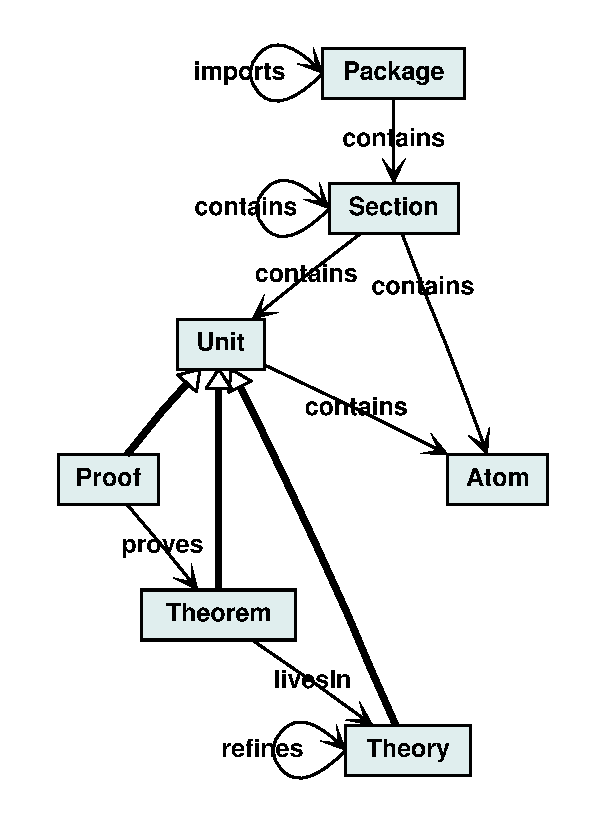
\includegraphics[width=.5\textwidth]{projects/semrelations/systems_onto_short}
    \end{minipage}
    \hspace*{-1cm}
    \begin{minipage}[b]{.4\textwidth}
      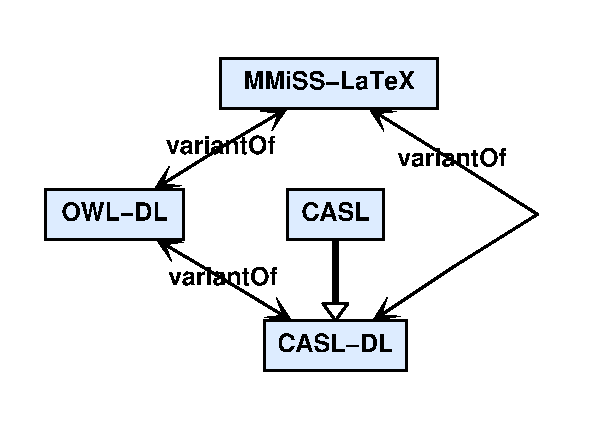
\includegraphics[width=1.1\textwidth]{projects/semrelations/onto_formalisms}
  \end{minipage}
  \caption{(a) Parts of the System's Ontology (b) Formalism variants}\label{fig:semrel-systems_onto}
\end{figure}

The next section will show, how we can explore this domain ontology --- supplied by the
author --- in order to capture semantic relations between document parts and use these
relations for supporting a management of change for mathematical documents.

\subsection{Change Management}

The notion of \emph{change management} is used for the maintenance and preservation of
consistency and completeness of a development during its evolution.  More precisely, we
want to have a {\twintoo{consistent}{configuration}} in which all versions are compatible
and there are no cyclic definitions or proofs.  At the same time, it should be a
{\twintoo{complete}{configuration}}: there should be no dangling forward references.

Such notions are well-known for formal languages. In contrast, natural language used for
writing teaching material does not usually possess a well-defined semantics, and the
notion of consistency is arguable.  Different authors may postulate different requirements
on the material in order to regard it as being consistent.  The existence of a
user-defined ontology helps a great deal to check references. However, we can make even
better use of the information contained in the ontology.

\paragraph{The System's Ontology}

The aim is to allow change management with regard to consistency and completeness
requirements defined by the user in terms of an ontology. In order to unify this approach
with the structural consistency and completeness properties introduced above, we express
the {\twintoo{document}{structure}}, originally defined by a document type definition, as
an ontology, the so-called \emph{System's Ontology} (see
Fig.~\ref{fig:semrel-systems_onto}a).  It defines the following relations between
structural elements of documents:
\begin{description}
\item [{\snippet{comprises}}] An obvious structuring mechanism is nesting of individual
  parts of a document, leading to the contains relation. The contains relation is part of
  a family of {\snippet{comprises}} relations that share common properties.
\item [{\snippet{reliesOn}}] A family of {\snippet{reliesOn}} relations reflects the
  various dependencies between different parts of a document.  For example, a theorem
  \emph{lives in} a theory, or proof \emph{proves} a theorem.
\item [{\snippet{pointsTo}}] The family of {\snippet{pointsTo}} relations is very similar,
  and relates references with the defining occurrence of a semantic term.
\item [{\snippet{variantOf}}] Another structuring relation is introduced by
  variants. Parts of a document may e.g. be written in various languages which gives rise
  to a {\snippet{variantOf}} relation between these document parts and their constituents;
  it is an equivalence relation.
\end{description}

It is now rather straightforward to formulate consistency and completeness rules in terms
of invariants of these relations. Formulating these invariants as formal rules will enable
us to implement a generic and flexible {\twintoo{change}{management}} that keeps track of
the invariants and informs the user about violations when a previously consistent document
has been revised, leading to various kinds of error (e.g. for {\snippet{reliesOn}}
relations) or warning messages (e.g. for {\snippet{pointsTo}} relations).


\paragraph{Properties of Interactions between Structuring Mechanisms.}
This approach also allows us to lift relations to structuring mechanisms allowing more
modular and localized change management.  For example, relating the {\snippet{comprises}}
and {\snippet{reliesOn}} relations allows us to formalize invariants regarding the closure
of document parts with respect to the {\snippet{reliesOn}} relation: We can require that
there is a proof for each theorem in a package.  Furthermore, if two structural entities
are related by {\snippet{reliesOn}}, their relation is propagated along the
{\snippet{comprises}} relation towards the root of the hierarchy of nested structural
entities, such that (for a theorem $T$ a proof $P$, and sections $A, B$):

\begin{description}
\item[] $B$ contains $P$ \& $A$ contains $T$ \& $P$ proves $T \Rightarrow B$
  {\snippet{reliesOn}} $A$.
\end{description}

% \[\text{B contains P and A contains T and P proves T, then
%         B reliesOn A.}
% \]

If the user changes section $A$, the repository will only need to check all sections that
$A$ relies on (such as $B$ here) for invariants, and not the whole document. However, in
contrast to formal developments as in e.g. the MAYA system \cite{AH-05-a}, there is no
rigorous requirement that a document should obey all the rules.  There may be good
reasons, for instance, to present first a "light-weight" introduction to all notions
introduced in a section before giving the detailed definitions. In this particular case,
one would want to introduce forward pointers to the definitions rather than making the
definitions rely on the introduction; thus the rules are covered.

In any case, the more structure there is, the better the chances are for preserving
consistency and completeness; any investment in introducing more {\snippet{reliesOn}}
relations, for example, will pay off eventually. The change management will observe
whether revisions by the user will affect these relations and, depending on the user's
preferences, emit corresponding warnings.

The aim is to allow users to specify individual notions of consistency by formulating the
rules that the relations should obey. This should be possible for the relations between
the particular (predefined) structuring mechanisms, but also in general between semantic
terms of the user's own ontology. Our work in this direction will rely on the methods and
tools provided by the {\hets} system (see {\mysecref{hets}}).

\subsection{Variants}

The concept of {\indextoo{variant}s} adds a new dimension to hierarchically
{\twintoo{structured}{document}s}.  The idea is to maintain and manage different variants
of structural entities (document subtrees) which represent the same information in
different ways --- variants are meant to glue them together.

Managing different natural language variants in parallel is an obvious example.  Another
one is the formalism variant which denotes the particular formalism in which a formal
content part like a theorem or a definition is expressed. Considering ontology development
itself, for example, we propose to use variants to maintain different formal
representations for the same semantic concept together with its documentation.
Figure~\ref{fig:semrel-systems_onto}b shows the possible variants for declaring ontology
components (see \cite{WOSE-2004} for details).

The \MMISS{} repository provides functions to store and retrieve these structural variants
by means of specifications for selecting particular variants for editing or presentation.

\subsection{Relations to {\omdoc}}

{\omdoc} provides modules for marking up the knowledge structure and the narrative
structure of mathematical documents. \MMISS{} combines these two viewpoints by giving
means for structuring the document contents (which constitutes the narrative structure) and
for specifying the incorporated knowledge by use of ontologies. Therefore, we have
implemented an export of \MMISS{} documents to (content and narrative) {\omdoc} documents
and vice versa.

% LocalWords:  MMiSS Bernd Krieg ckner Achim Mahnke multi reliesOn pointsTo
% LocalWords:  variantOf hets subtrees versa

\end{projectdescription}

\begin{projectdescription}
  %%%%%%%%%%%%%%%%%%%%%%%%%%%%%%%%%%%%%%%%%%%%%%%%%%%%%%%%%%%%%%%%%%%%%%%%%
% This file is part of the LaTeX sources of the OMDoc 1.3 specifiation
% Copyright (c) 2006 A.M. Cohen, H. Cuypers, E. Reinaldo Barreiro
% This work is licensed by the Creative Commons Share-Alike license
% see http://creativecommons.org/licenses/by-sa/2.5/ for details
\svnInfo $Id: mathdox2.tex 8453 2009-08-04 09:58:26Z kohlhase $
\svnKeyword $HeadURL: https://svn.omdoc.org/repos/omdoc/branches/omdoc-1.3/doc/spec/projects/mathdox/mathdox2.tex $
%%%%%%%%%%%%%%%%%%%%%%%%%%%%%%%%%%%%%%%%%%%%%%%%%%%%%%%%%%%%%%%%%%%%%%%%%

\section[MathDox]{MathDox: Mathematical Documents on the Web}
\begin{project}{mathdox2}{http://www.mathdox.org}
\pauthors{A.M. Cohen, H. Cuypers, E. Reinaldo Barreiro}
\pinstitute{Department of Mathematics and Computer Science, Eindhoven University of Technology}
\end{project}
\renewcommand{\CAS}{\indextoo{CAS}}


\begin{pabstract}
  The {\MathDox} system provides an infrastructure for
  {\atwintoo{interactive}{mathematical}{document}s} that make use of the World Wide Web.
  These documents take input from various sources, users, and mathematical services.
  Communication between these different entities can be realized using {\openmath}.  But,
  such {\indextoo{communication}} and the {\indextoo{interactivity}} inside the
  mathematical document take place in a specific, dynamic context. In this paper we
  discuss our approach to such a {\atwintoo{dynamic}{mathematical}{context}}: {\MathDox}.
  It consists of both an {\xml}-based markup language for interactive mathematical
  contents and a set of software tools realizing the interactivity.
\end{pabstract}



\subsection{Introduction}
Although the notion of an interactive mathematical document has been around for several
years, cf.~\cite{CohMee:tapap98}, its realization is nowhere near the final stage. For
instance, recent progress in web technologies has enabled a much smoother communication of
mathematics than ever before. The use of an interactive mathematical document (IMD) can
provide a window to the world of mathematical services on the Internet, and a mathematical
service on the Internet can be created by the building of an interactive mathematical
document.  {\MathDox} is an ensemble of software tools for creating IMDs, it includes
\begin{enumerate}
\item an {\xml} based language that offers markup support for the source texts of IMDs;
\item a document server, rendering interactive mathematical documents from source text and
  interactively obtained information;
\item mathematical services, providing connections with {\CAS{s}} like {\mathematica} and
  {\gap} via {\openmath} phrasebooks (cf.~\cite{URL:omsoc}).
\end{enumerate}

The creation of {\MathDox} is a project at the Technische Universiteit Eindhoven (the
RIACA institute).  Several people at RIACA have helped creating it; here we mention
Manfred Riem, Olga Caprotti, Hans Sterk, Henny Wilbrink, Mark Spanbroek, Dorina Jibetean.
The system is mainly built with Java and related technology.  The products are available
via the project web site and will be licensed under the Lesser Gnu Public
License~\cite{LGPL}.


\subsection{The Language}\label{uisection}
The \MathDox\ source is an \xml\ document.  We have derived our own document type
definitions (DTD) for these source texts.  We have been influenced by both
{\docbook}~\cite{WalMue:dtdg99} and {\omdoc}. The former is a fairly general standard for
electronic books, the latter is a very rich, and strongly logic-oriented standard for
mathematical documents---the main subject of this book.  Both {\omdoc} and {\MathDox} use
{\openmath}~\cite{BusCapCar:2oms04}, the difference being that {\omdoc} focuses on
representing mathematical knowledge whereas {\MathDox} focuses on interactivity.  The
connections with both DocBook and {\omdoc} are of importance to us because we expect
several authoring tools for it to emerge in the coming few years, and we want to profit
from their presence.

The mathematics in the {\MathDox} source is given by means of {\openmath} objects.  This
feature has clear advantages in terms of portability. The DocBook type grammar sees to it
that there are natural scopes, where mathematical objects `live'. For instance, when a
chapter begins with ``Let $\mathbb{F}$ be a field'', the scope of the variable
$\mathbb{F}$ is assumed to be the whole chapter (although, somewhere further down the
hierarchy, say in a section of the chapter, this assignment can be overridden).

Interactivity in {\MathDox} is taken care of by {\xml} tags representing various
{\twintoo{programming}{construct}s} as well as queries to
{\atwintoo{external}{mathematical}{service}s}.  These actions take place within part of
the context, which fixes the precise semantics of the objects involved.  Further
constructs are available for handling context and user input.  Our notion of context is
based on \cite{FraHes:aoidms99}. Context is divided into static\twin{static}{context} and
{\twintoo{dynamic}{context}}. The static context may be defined as the set of all {\xml}
sources from which a interactive document can be prepared for use. Two extreme forms are
{\openmath} Content Dictionaries\twin{content}{dictionary} and a chapter of an ordinary
book.  The dynamic context behaves more like the {\indextoo{state}} of a {\CAS}.  It
keeps track of the variables introduced, their properties, their values, and their scopes.
The {\MathDox} language has constructs for storing and changing this information.  For
example, the field $\mathbb{F}$ introduced at the beginning of a chapter may be specified
to be a finite field of five elements in the context of a particular section of the
chapter.

Although semantics is the primary target, some features for presentation have been built
into the language.  In order to have a flexible presentation, we use
presentation-annotated {\openmath}.  In \MathDox\ we allow style attributes inside
{\openmath} objects.  By discarding these style attributes, regular {\openmath} is
obtained. For instance, by providing the appropriate value for the style attribute, the
author has a choice between a slash and a fraction display. In $\frac{3/4+2/3}{5}$ we have
used them both.

Another way of solving presentation issues is illustrated by the statement:
$3,4\in\mathbb{Z}$.  The corresponding {\openmath} expression would be the equivalent of
$3\in\mathbb{Z} \wedge 4\in\mathbb{Z}$, but our {\openmath} statement reads that the
sequence $3,4$ belongs to $\mathbb{Z}$.  So here, the semantics of the element-of symbol
has been stretched so as to help out presentation.


\subsection{The {\MathDox} System}\label{subsec:cont_theory:mathdox}

An essential component of the {\MathDox} software is its {\twintoo{document}{server}}. It
provides a view to the client of the content and manages both the
static\twin{static}{context} and the {\twintoo{dynamic}{context}}.  The usage of the
{\MathDox} document server is shown in {\myfigref{DocModel}}. We explain in some detail
the main components shown in this picture.


\begin{myfig}{DocModel}{The {\MathDox} software}
  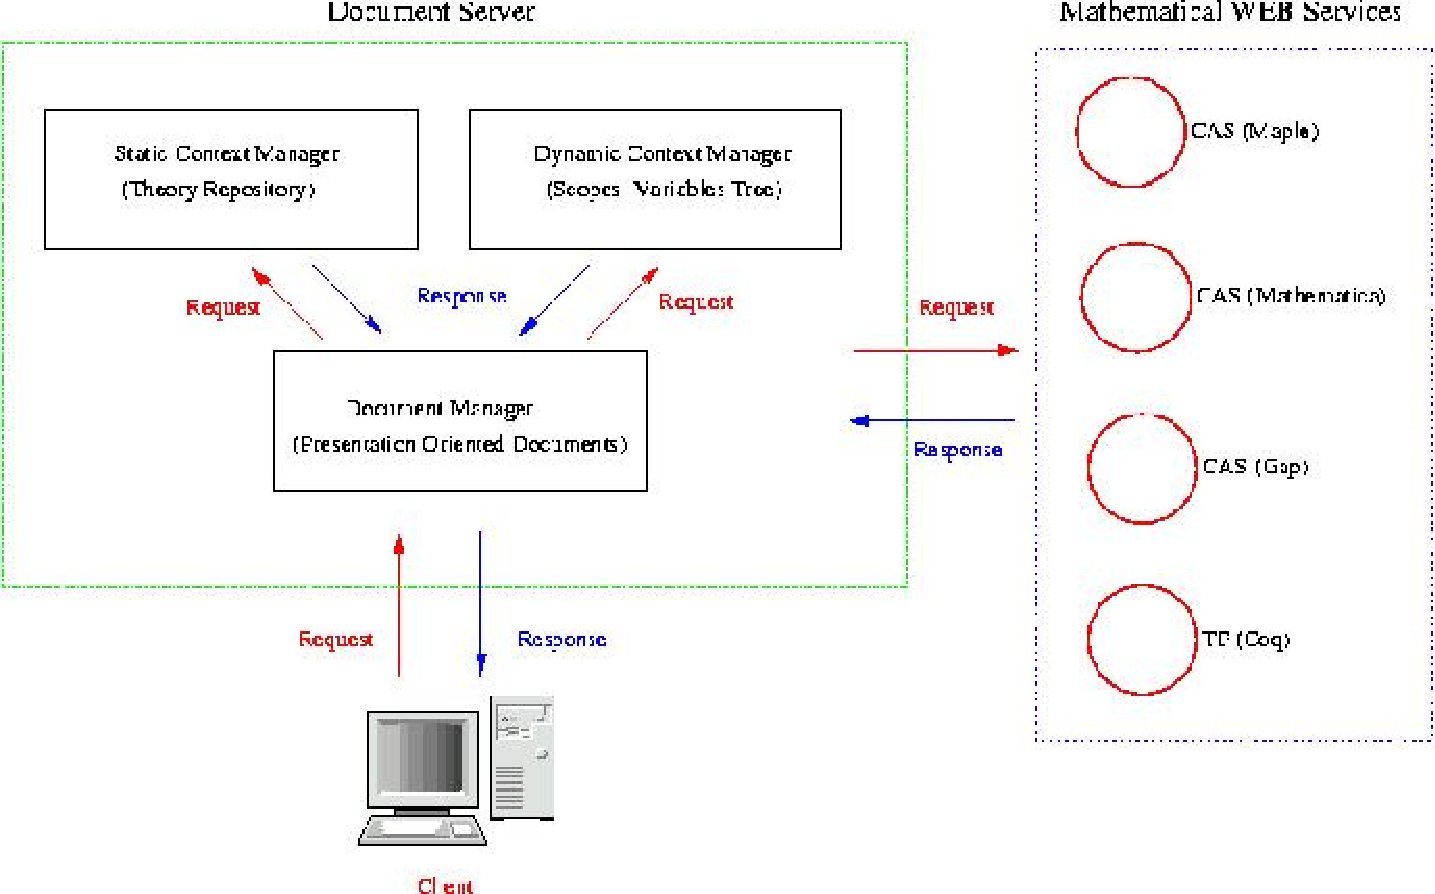
\includegraphics[width=11cm]{projects/mathdox/DocModel}
\end{myfig}

\begin{enumerate}
\item The {\emin{client}}. The client is realized by a
  {\atwintoo{math-enabled}{web}{browser}}.  It will present views of the documents served
  to the user, interact with the user, and communicate user input to the document server.

  The communication between client and server takes place via the HTTP request/response
  mechanism.  The responsibility for interaction is mostly on the server side.
\item The {\twinemph{document}{server}}.  This server caters for presentation,
  communication, and context.  It supports a wide range of actions ranging from handling
  queries to searching within documents for mathematical content and from placing (and
  retrieving) objects into the context, to rendering documents in different views.

  The document server is realized as a Java enhanced
  {\twintoo{web}{application}}~\cite{URL:jsp} inside a web server.  It is not a monolithic
  entity. As shown in {\myfigref{DocModel}}, it is formed by the system parts.  The
  {\twinemph{document}{manager}} serves views to the client.  IMDs can be thought of
  as programs (scripts) encoding the production of a response.  In generating the
  response, they can make use of the information contained in the static context, and in
  the dynamic context (scopes and variables), the user input communicated along with
  request, and the results of computations carried on by one or more mathematical
  services.
  
  Another part is the {\atwinemph{static}{context}{manager}} which is responsible
  for managing a repository of {\MathDox} mathematical theories.
  
  The final (third) part is the {\atwinemph{dynamic}{context}{manager}} which is
  responsible for the dynamic information.

\item {\em\twintoo{mathematical}{service}s}.  Mathematical services can be very diverse:
  some may serve as general interfaces to {\CAS} or to Theorem Provers.  The {\MathDox}
  software provides ways to access these services via standard protocols, among which
  those developed under the MONET project~\cite{URL:monet}.  The mechanism extends the
  phrasebook set-up for {\openmath}~\cite{CapCoh:uosdmc00,CapCoh:jpcaad00}.  For
  constructing specific {\openmath} services, we employ our Java {\openmath} library
  ROML~\cite{URL:roml}.
\end{enumerate}

\subsection{Conclusion}
Now that {\MathDox} is close to a complete working version, trial applications are in the
make. We mention
\begin{itemize}
\item a server for providing designs of experiments on command to statisticians,
\item an exercise repository for the EU funded LeActiveMath project,
\item a mathematics course on calculus, with automated natural language production from a
  formal-mathematical source for the EU funded project WebALT,
\item interactive lecture notes (the successor of~\cite{CohCuySterk:ida99}) for an
  Abstract Algebra course within a mathematically oriented Bachelor curriculum,
\item educational material for highschool mathematics in the Netherlands.
\end{itemize}




%%% Local Variables: 
%%% mode: latex
%%% TeX-master: "../../omdoc"
%%% End: 








% LocalWords:  MathDox mathdox Cuypers Barreiro Eindhoven IMD IMDs CAS DocBook
% LocalWords:  cf phrasebooks Technische Universiteit RIACA Riem Caprotti Sterk
% LocalWords:  Henny Wilbrink Spanbroek Dorina Jibetean DTD HTTP phrasebook ath
% LocalWords:  ROML LeActiveMath WebALT highschool hrasebooks omputer lgebra pp
% LocalWords:  utomated eduction SIGSAM Rom Arjeh ATCM Chiang Chu Jen Chuan eds
% LocalWords:  ISBN Meertens ACELA Kajler Wien JavaServer Franke Ch Sorge vol
% LocalWords:  sk mathdox DocModel mathdox mathdox mathdox mathdox

\end{projectdescription}

\begin{projectdescription}
  %%%%%%%%%%%%%%%%%%%%%%%%%%%%%%%%%%%%%%%%%%%%%%%%%%%%%%%%%%%%%%%%%%%%%%%%%
% This file is part of the LaTeX sources of the OMDoc 1.3 specifiation
% Copyright (c) 2006 Christoph Lange
% This work is licensed by the Creative Commons Share-Alike license
% see http://creativecommons.org/licenses/by-sa/2.5/ for details
\svnInfo $Id: main.tex 8453 2009-08-04 09:58:26Z kohlhase $
\svnKeyword $HeadURL: https://svn.omdoc.org/repos/omdoc/branches/omdoc-1.3/doc/spec/projects/swim/main.tex $
%%%%%%%%%%%%%%%%%%%%%%%%%%%%%%%%%%%%%%%%%%%%%%%%%%%%%%%%%%%%%%%%%%%%%%%%%

\section{{\swim} -- An OMDoc-based Semantic Wiki}
\begin{project}{swim}{http://kwarc.eecs.iu-bremen.de/projects/swim}
\pauthors{Christoph Lange\and Michael Kohlhase}
\pinstitute{Computer Science, International University Bremen}
\end{project}

{\swim} is a semantic wiki for collaboratively building, editing and browsing a
mathematical knowledge base of {\omdoc} theories. Our long-term objective is to develop a
software that facilitates the creation of a shared, public collection of mathematical
knowledge and serves work groups of mathematicians as a tool for collaborative development
of new theories.  Even though the work reported here was initially motivated by solving
the MKM author's dilemma~\cite{KohKoh:cdad04}, we contend that the new application area
MKM can also contribute to the development of semantic wikis.

Technically, {\swim} is based on the semantic wiki engine
\scsys{IkeWiki}~\cite{schaffert06:ikewiki}, which was chosen because of its
modular design, its rich semantic web infrastructure, its user assistance for
annotations, and its orientation towards
learning~\cite{schaffert06:learning-with-semantic-wikis}.

\subsection{Semantic Wikis}

A wiki~\cite{LeuCun01:wikiway} is a web server
application that allows users to browse, create, and edit hyperlinked pages in a web
browser, usually using a simple text syntax.  In contrast to most content management
systems, wiki pages are accessible via an URL containing their title.  A new page can be
created by linking from an existent page to the page to be created.  This link will then
lead to an edit form.  Usually, anyone is allowed to edit pages on a wiki, but access can
be restricted.  Other characteristics of wikis include permanent storage of old page
versions (with facilities to display differences between two versions and to restore a
certain version), notification about recent changes, and full-text search.

Semantic
wikis~\cite{voelkel06:semanticwikistateoftheart,TolPas06:wikis-semantic-hypermedia}
enhance wikis by Semantic Web technologies, such as {\rdf}~\cite{LasSwi:rdf99} or
ontologies.  Usually one page represents one concept from a real-world domain, which has a
type, possibly some metadata, and typed links to other concepts.  For example, a link from
a wiki page about ``Life, the Universe and Everything'' to another page about Douglas
Adams could be typed as ``is author of''.  In terms of {\rdf}, this can be expressed by the
following subject--predicate--object triple,

\[
(\mbox{``Douglas Adams''},\;\mbox{isAuthorOf},\;\mbox{``Life, the Universe and
Everything''})
\]

where the \textit{isAuthorOf} relation would be defined in an ontology.  These links are
usually displayed in a navigation box next to the page contents. Semantic wikis only deal
with wiki text, not with mathematics, though some allow to embed mathematical formulae as
presentational-only {\TeX}.

{\swim} encourages users to collaborate: Non-mathematicians can collaborate in creating a
``Wikipedia of mathematics'' by compiling the knowledge available so far, while scientists
can collaboratively develop new theories.  Users get an immediate reward for many of their
contributions: Once they specify the type of a page or relations of one page to another,
this information will be displayed in a box of navigation links.  We intend to make the
data created in {\swim} usable for external services by offering an export facility for
{\omdoc} documents and by integrating them into {\swim}.  Mathematicians developing
theories will be assisted to retain an overview of theory dependencies in order not to
break them.  Social software services will further utilize the semantic information
available from the theories and from tracking the user interaction log (``Who did what on
which page when?'').  User feedback to pages can be extended to social bookmarking, which
is ``the practice of saving bookmarks [of Internet resources] to a public web site and
`tagging' them with keywords.''~\cite{lomas05:social-bookmarking} The more users tag a
certain resource, the higher a social bookmarking service will rank it.

The enhancements of the data model semantic wikis bring along --- compared to traditional
wikis --- are already present in the {\omdoc} format, so that an {\omdoc}-based wiki only
needs to operationalize their underlying meaning. For example, typed links, which are
implemented via an extension to the wiki syntax in \scsys{Semantic
  MediaWiki}~\cite{voelkel06:semanticwikipedia} or editable through a separate editor in
\scsys{IkeWiki}~\cite{schaffert06:ikewiki}, are implemented by means of the \texttt{for}
attribute to {\omdoc}'s elements (e.g.\ \texttt{<example for="\#id-of-assertion">}).
{\swim} makes them editable easily and visualizes them adequately.  A semantic wiki
targeted at mathematics must ensure that dependencies between concepts are preserved.
Results in this area will be interesting for non-mathematical semantic wikis as well,
especially when they support higher levels of formalization such as ontologies.

\subsection{Design of {\swim}}

\subsubsection{Concepts and Relations}

The smallest unit that can be displayed, edited, linked to, or archived in a wiki is a
page. In a semantic wiki, it usually describes one {\emph{concept}}, including its
properties and its relations to other concepts.  While standalone {\omdoc} documents can
contain more than one theory, is is important to keep pages small in a wiki to improve the
effectivity of usage.  Furthermore, usual semantic wikis only store and display metadata
and typed links per page; {\swim} does too.\footnote{Semantic information will only be
  considered on the theory and statement levels of {\omdoc} --- directly or through
  reasoning in the case of transitive closures ---, not on the object level.}  Users are
strongly encouraged to define at most one theory per wiki page and to roll out
non-constitutive statements (see {\mysecref{statements-constitutive}}) to separate pages,
referencing their context theory.  As constitutive statements cannot exist without an
enclosing theory, but as, on the other hand, we want each wiki page to form a valid
document, we introduced a new element {\element[ns-elt=swim]{page}}, which can be a child
of an {\element{omdoc}} element and which has the same content model as a
{\element{theory}} element --- in particular, it can hold several theory-constitutive
statements and connect them to their context theory.
\begin{wrapfigure}{r}{8cm}
  \begin{tikzpicture}[scale=1.5,thin,font=\sffamily,>=triangle 60]
    \tikzstyle{concept}=[font=\sffamily\bfseries,draw,minimum height=3.5ex,rounded corners]
    \tikzstyle{every path}=[font=\small\sffamily];
    \node[concept] (t) at (0,1) {theory};
    \node[concept,dashed] (s) at (0,0) {\itshape statement};
    \node[concept] (d) at +(-158:2.0cm) {definition};
    \begin{scope}[shift={(d)}]% control point for e->d
      \coordinate (da) at +(-90:1.5cm);% relative to s, not to a!
    \end{scope}
    \node[concept] (a) at +(-120:1.5cm) {assertion};
    \begin{scope}[shift={(a)}]% control point for e->a
      \coordinate (aa) at +(-30:1cm);% relative to s, not to a!
    \end{scope}
    \node[concept] (p) at +(-60:1.5cm) {proof};
    \node[concept] (e) at +(-22:2.0cm) {example};
    \draw[->] (t.-60) .. controls +(-60:0.5cm) and +(-30:0.5cm) .. node[right]
    {imports} (t.east);
    \draw[->] (s) -- node[left] {context for} (t);
    \draw[-open triangle 60] (d) -- node[above] {is a} (s);
    \draw[-open triangle 60] (a) -- node[above left] {is a} (s);
    \draw[-open triangle 60] (p) -- node[above right] {is a} (s);
    \draw[-open triangle 60] (e) -- node[above] {is a} (s);
    \draw[->] (p) -- node[above] {proves} (a);
    \draw[->] (e) ..
    controls +(-120:1cm)
    and (aa) ..
    node[below left] {exemplifies} (a);
    \draw[->] (e) ..
    controls +(-90:1.5cm)
    and (da) ..
    node[below left] {exemplifies} (d);
  \end{tikzpicture}
  \caption{Subset of {\omdoc}'s system ontology}\vspace*{-.5cm}
\end{wrapfigure}
{\omdoc}'s system ontology has been partly coded in OWL-DL and imported to the wiki's {\rdf}
store, which is implemented using the Jena Semantic Web Framework for
Java~\cite{URL:jena:web}. Theories as well as statements of any type form concepts, and
the most important relations between those concepts are extracted from the {\omdoc} pages
on saving and then stored as {\rdf} triples.  These relations include:
\begin{itemize}
\item The import relation between theories
\item The relation of a statement to its context theory
\item The relation of an example to the statement it exemplifies
\item The relation of a proof to the assertion it proves
\end{itemize}
It is planned to also take relations given by user interaction into consideration, such as
``Who edited which page when?'', and to combine ontology-defined relations and user
relations.  For example, a metric estimating the {\emph{degree of difficulty}} of a page,
calculated by counting the questions on the discussion page, could be implemented.
Furthermore, the user can specify taxonomic relations, which cannot be stated explicitly
in {\omdoc}, such as (``all differentiable functions are continuous''), as annotations in
an ontology language like {\rdf} Schema or {\owl}.

\subsubsection{User Interface and Interaction Model}

Pages can be rendered to XHTML plus presentational MathML using the transformations
described in {\mychapref{transform-xsl}}. There is also a browsable source code view, which is
useful for documents that are not written in textbook style.

Not only will the user be able to navigate along the dependency graph, she will also be
able to {\emph{interact}} with the system: she will be asked whether she wants to explore
the theories required as dependencies in further detail.

Suppose that the user is currently reading the page containing the theory {\snippet{ring}}
from the elementary algebra example from {\mychapref{dg-elal}}. In this case the wiki will
not only display navigation links to the direct dependencies {\snippet{group}} and
{\snippet{monoid}}, but it will also provide unobtrusive buttons that allow the user to
give one of the commands in {\myfigref{gui-showdeps}}. Not only the last case will be
recorded --- the others are interesting as well for \emph{social bookmarking}.  For
example, if many users requested a theory $t$ to be explained, the system could default to
display not only the direct dependencies but also the level-two dependencies, for it seems
that $t$ is too difficult for only being explained shallowly.

\begin{myfig}{gui-showdeps}{The command buttons to navigate along the dependencies}
  \begin{minipage}{8cm}
\begin{description}
\item[{\bf{No, thanks!}}] ``{\emph{I already know group and monoid.}}''
\item[{\bf{Explain}}] ``{\emph{Please show me group and monoid, I want to learn about
      ring's prerequisites.}}'' --- group and monoid will be displayed.
\item[{\bf{Explore}}] ``{\emph{Please show me {\emph{all}} prerequisites for ring.}}'' ---
  group, monoid, and semigroup, are opened in separate windows or serialized into one
  page.
\item[{\bf{Suspend}}] ``{\emph{I want to know about group and monoid, but only later.}}''
  --- {\swim} keeps a notice in the user's profile that she wants to read group and monoid
  sometime.  Reminder links to suspended theories are shown on a separate navigation bar.
\end{description}
\end{minipage}\quad
\begin{minipage}{2.5cm}
  
\includegraphics[width=2.5cm]{projects/swim/gui-showdeps}
\end{minipage}
\end{myfig}

\subsubsection{Further work}

Further work on {\swim} will concentrate on integrating a lightweight
management of change process.  Second, while the wiki is yet a user-friendly
\emph{browser}, there is still a demand for assisting users to \emph{edit}
{\omdoc}.  To this end, the {\qmath} preprocessor (see {\mysecref{qmath}}) will
be integrated into {\swim}.  Mathematical objects entered as {\qmath} will be
kept in this syntax for display in the edit form, but they will be converted to
{\omdoc} for rendering for presentation and when pages are exported to another
application.

%%% Local Variables: 
%%% mode: stex
%%% TeX-master: "../../omdoc"
%%% End: 

% LocalWords:  matwebsearch Ioan Sucan nC dx dy dt runningex XPointer ns attr
% LocalWords:  mq anyorder xmlns domainofapplication bvar ci cn eq OAI API da
% LocalWords:  Lange CPoint wikis dateness parseable isAuthorOf MediaWiki omdoc
% LocalWords:  aa wiki's Wiki wiki IkeWiki JA hypermedia elt semithick pres dg
% LocalWords:  elal gui showdeps qmath stex metadata wiki's scheint mir kein zu
% LocalWords:  Gegensatz sein

\end{projectdescription}

\begin{projectdescription}
  %%%%%%%%%%%%%%%%%%%%%%%%%%%%%%%%%%%%%%%%%%%%%%%%%%%%%%%%%%%%%%%%%%%%%%%%%
% This file is part of the LaTeX sources of the OMDoc 1.3 specifiation
% Copyright (c) 2006 Paul Libbrecht
% This work is licensed by the Creative Commons Share-Alike license
% see http://creativecommons.org/licenses/by-sa/2.5/ for details
\svnInfo $Id: authoring.tex 8453 2009-08-04 09:58:26Z kohlhase $
\svnKeyword $HeadURL: https://svn.omdoc.org/repos/omdoc/branches/omdoc-1.3/doc/spec/projects/activemath/authoring.tex $
%%%%%%%%%%%%%%%%%%%%%%%%%%%%%%%%%%%%%%%%%%%%%%%%%%%%%%%%%%%%%%%%%%%%%%%%%

\section{Authoring Tools for {\activemath}}
\begin{project}{jeditoqmath}{http://www.activemath.org/projects/jEditOQMath}
  \pauthors{Paul Libbrecht} 
  \pinstitute{DFKI GmbH and Universit{\"a}t des Saarlandes}
\end{project}


The {\omdoc} content to be delivered by {\activemath} are {\omdoc} documents with
{\openmath} formulae. Experience has shown that writing the {\xml}-source by hand is
feasible and even preferred if the author wants to follow the evolution of content's
structure.  It is similar to {\html} editing.  However, the complexity of {\xml} makes it
hard to keep an overview when writing mathematical expressions. Therefore, the
{\scsys{OQMath}} processor has been implemented: it uses {\scsys{QMath}} for formulae and
leaves the rest of the {\omdoc} written as usual {\xml}.

{\scsys{OQMath}} has been integrated in a supporting {\xml}-editor, jEdit. This editor
provides structural support at writing {\xml}-documents. Authors, even with no
{\xml}-knowledge, can easily write valid document {\scsys{jEditOQMath}}.  This package
includes, in a one-click installer, {\qmath}, {\scsys{OQMath}}, {\scsys{jEdit}}, and
Ant-scripts for publication of the content in {\activemath} knowledge bases.  These
scripts validate the references in the content.  These scripts also provide authors with
short cycles edit-in-{\scsys{jEditOQMath}}-and-test-in-{\activemath}.  More about
{\scsys{jEditOQMath}} can be seen from
{\url{http://www.activemath.org/projects/jEditOQMath}} at~\cite{AM-authoring-from-dev-on}

%Explorations of knowledge navigation and edition using the Protege%
%\footnote{See \url{http://protege.semanticweb.org/}.}
%ontology editor
%have been made but limitations of the visualization library have plagued this first visual
%editor attempts.

%Access to the other {\omdoc} content in order for them to be referenced, used, or inspected
%has turned out to be an essential requirement of authoring tools: 
{\scsys{jEditOQMath}} provides search facilities as well as contextual drops from items
presented in an {\activemath} window.  This way the testing of content in the target
environment and the authoring experience are bound tighter together,
% binds even tighter the test-running of content in the environment where it will be
%delivered to the authoring experience, 
thus making {\scsys{jEditOQMath}} closer to the WYSIWYG paradigm without being limited to
its simple visual incarnation.

%exercise authoring tool for 'authoring by demonstration'
%---- Ian or George here ----
% George: I can not write anything yet, there is no version of a tool releazed

% abundant  experience with authors
To date, more than $10'000$ {\emph{items}} of {\omdoc} content has been written using
these authoring tools in Algebra and Calculus. This experience with authors considerably
improved our understanding of what today's authors need and what different classes of
authors can cope with.

% has allowed us to
% gear features of the authoring tools towards users and has shown gaps still to be filled.

Among the greatest difficulties of authoring content for {\activemath} was the art of
properly choosing mathematical semantic encoding: the mathematical discourse is made of
very fine notation rules along with subtle digressions to these rules...  formalizing
them, as is needed when writing {\openmath} or the {\qmath} formulae for them, turns out
to often be overwhelming.  The usage of the ellipsis in such a formula as $1, \dots, k,
\dots, n$ is a simple example of semantic encoding challenge. The knowledge organization
of {\omdoc} that makes it possible to define one's own {\openmath} symbols has been a key
ingredient to facing this challenge.

Among the features most requested by authors, which we have tried to answer 
as much as possible,  are a short edit-and-test cycle and validation facilities 
taking in account the overall content.

\subsubsection{Validation Tools}

Automated validation of {\omdoc} content has many facets.
% can be done in many respects but little has been done with {\omdoc} documents.
{\xml}-validation with a DTD and Schema is a first step.  However there are still many
structure rules mentioned only as human readable forms in the {\omdoc} specifications.
References between {\omdoc} items is another important facet which has been answered by
{\activemath} knowledge bases and publishing scripts.  Experience has proved that ignoring
such errors has lead repeatedly to authors complaining about the weirdest behaviours of
the overall learning environment.  Many other simple validations could be done in order to
support the author, for example the validation of a picture embedding, or of fine grained
typing of relations (for example, that a definition should only be {\emph{for}} a symbol).

Further validation tools are being investigated, for example, those tuned to particular
pedagogical scenarios.


\subsubsection{Further Authoring Tools for {\activemath}} {\scsys{jEditOQMath}} clearly
remains for users who feel comfortable with source editing. Experience has shown that
authors having written {\html} or {\TeX} earlier did not find this paradigm problematic.
It is, however, a steep learning slope for beginner authors.  A more visual component is
being worked upon, able to display and edit visually the children of a \element{CMP},
including formulae.\footnote{More about the component for {\omdoc} micro-structure can be
  read from \url{http://www.activemath.org/projects/OmdocJdomAuthoring/}.}  This
component, along with forms and summaries for metadata, should provide a visual
environment to edit {\omdoc} content for {\activemath} in a relatively accessible way.

Another area where source editing has shown difficulties is in the process of authoring
exercises with many steps... the rich structure of the exercises, along with the non-neglect able
space taken by the display of {\xml}-source has challenged several authors, having
difficulties to overview such sources as 600 Kb of {\scsys{OQMath}} source for a single
exercise. 
A web-based visual authoring environment is under work within the {\activemath} group.

%%% Local Variables: 
%%% mode: stex
%%% TeX-master: "../../omdoc"
%%% End: 

% LocalWords:  jeditoqmath Libbrecht GmbH Universit des Saarlandes OQMath QMath
% LocalWords:  jEdit jEditOQMath jEditOQMath jEditOQMath jEditOQMath one's
% LocalWords:  jEditOQMath jEditOQMath jEditOQMath jEditOQMath jEditOQMath
% LocalWords:  jEditOQMath jEditOQMath jEditOQMath metadata jEditOQMath
% LocalWords:  jEditOQMath jEditOQMath jEditOQMath jEditOQMath jEditOQMath

\end{projectdescription}

\begin{projectdescription}
  %%%%%%%%%%%%%%%%%%%%%%%%%%%%%%%%%%%%%%%%%%%%%%%%%%%%%%%%%%%%%%%%%%%%%%%%%
% This file is part of the LaTeX sources of the OMDoc 1.3 specifiation
% Copyright (c) 2006 Christoph Lange
% This work is licensed by the Creative Commons Share-Alike license
% see http://creativecommons.org/licenses/by-sa/2.5/ for details
\svnInfo $Id: main.tex 8453 2009-08-04 09:58:26Z kohlhase $
\svnKeyword $HeadURL: https://svn.omdoc.org/repos/omdoc/branches/omdoc-1.3/doc/spec/projects/swim/main.tex $
%%%%%%%%%%%%%%%%%%%%%%%%%%%%%%%%%%%%%%%%%%%%%%%%%%%%%%%%%%%%%%%%%%%%%%%%%

\section{{\swim} -- An OMDoc-based Semantic Wiki}
\begin{project}{swim}{http://kwarc.eecs.iu-bremen.de/projects/swim}
\pauthors{Christoph Lange\and Michael Kohlhase}
\pinstitute{Computer Science, International University Bremen}
\end{project}

{\swim} is a semantic wiki for collaboratively building, editing and browsing a
mathematical knowledge base of {\omdoc} theories. Our long-term objective is to develop a
software that facilitates the creation of a shared, public collection of mathematical
knowledge and serves work groups of mathematicians as a tool for collaborative development
of new theories.  Even though the work reported here was initially motivated by solving
the MKM author's dilemma~\cite{KohKoh:cdad04}, we contend that the new application area
MKM can also contribute to the development of semantic wikis.

Technically, {\swim} is based on the semantic wiki engine
\scsys{IkeWiki}~\cite{schaffert06:ikewiki}, which was chosen because of its
modular design, its rich semantic web infrastructure, its user assistance for
annotations, and its orientation towards
learning~\cite{schaffert06:learning-with-semantic-wikis}.

\subsection{Semantic Wikis}

A wiki~\cite{LeuCun01:wikiway} is a web server
application that allows users to browse, create, and edit hyperlinked pages in a web
browser, usually using a simple text syntax.  In contrast to most content management
systems, wiki pages are accessible via an URL containing their title.  A new page can be
created by linking from an existent page to the page to be created.  This link will then
lead to an edit form.  Usually, anyone is allowed to edit pages on a wiki, but access can
be restricted.  Other characteristics of wikis include permanent storage of old page
versions (with facilities to display differences between two versions and to restore a
certain version), notification about recent changes, and full-text search.

Semantic
wikis~\cite{voelkel06:semanticwikistateoftheart,TolPas06:wikis-semantic-hypermedia}
enhance wikis by Semantic Web technologies, such as {\rdf}~\cite{LasSwi:rdf99} or
ontologies.  Usually one page represents one concept from a real-world domain, which has a
type, possibly some metadata, and typed links to other concepts.  For example, a link from
a wiki page about ``Life, the Universe and Everything'' to another page about Douglas
Adams could be typed as ``is author of''.  In terms of {\rdf}, this can be expressed by the
following subject--predicate--object triple,

\[
(\mbox{``Douglas Adams''},\;\mbox{isAuthorOf},\;\mbox{``Life, the Universe and
Everything''})
\]

where the \textit{isAuthorOf} relation would be defined in an ontology.  These links are
usually displayed in a navigation box next to the page contents. Semantic wikis only deal
with wiki text, not with mathematics, though some allow to embed mathematical formulae as
presentational-only {\TeX}.

{\swim} encourages users to collaborate: Non-mathematicians can collaborate in creating a
``Wikipedia of mathematics'' by compiling the knowledge available so far, while scientists
can collaboratively develop new theories.  Users get an immediate reward for many of their
contributions: Once they specify the type of a page or relations of one page to another,
this information will be displayed in a box of navigation links.  We intend to make the
data created in {\swim} usable for external services by offering an export facility for
{\omdoc} documents and by integrating them into {\swim}.  Mathematicians developing
theories will be assisted to retain an overview of theory dependencies in order not to
break them.  Social software services will further utilize the semantic information
available from the theories and from tracking the user interaction log (``Who did what on
which page when?'').  User feedback to pages can be extended to social bookmarking, which
is ``the practice of saving bookmarks [of Internet resources] to a public web site and
`tagging' them with keywords.''~\cite{lomas05:social-bookmarking} The more users tag a
certain resource, the higher a social bookmarking service will rank it.

The enhancements of the data model semantic wikis bring along --- compared to traditional
wikis --- are already present in the {\omdoc} format, so that an {\omdoc}-based wiki only
needs to operationalize their underlying meaning. For example, typed links, which are
implemented via an extension to the wiki syntax in \scsys{Semantic
  MediaWiki}~\cite{voelkel06:semanticwikipedia} or editable through a separate editor in
\scsys{IkeWiki}~\cite{schaffert06:ikewiki}, are implemented by means of the \texttt{for}
attribute to {\omdoc}'s elements (e.g.\ \texttt{<example for="\#id-of-assertion">}).
{\swim} makes them editable easily and visualizes them adequately.  A semantic wiki
targeted at mathematics must ensure that dependencies between concepts are preserved.
Results in this area will be interesting for non-mathematical semantic wikis as well,
especially when they support higher levels of formalization such as ontologies.

\subsection{Design of {\swim}}

\subsubsection{Concepts and Relations}

The smallest unit that can be displayed, edited, linked to, or archived in a wiki is a
page. In a semantic wiki, it usually describes one {\emph{concept}}, including its
properties and its relations to other concepts.  While standalone {\omdoc} documents can
contain more than one theory, is is important to keep pages small in a wiki to improve the
effectivity of usage.  Furthermore, usual semantic wikis only store and display metadata
and typed links per page; {\swim} does too.\footnote{Semantic information will only be
  considered on the theory and statement levels of {\omdoc} --- directly or through
  reasoning in the case of transitive closures ---, not on the object level.}  Users are
strongly encouraged to define at most one theory per wiki page and to roll out
non-constitutive statements (see {\mysecref{statements-constitutive}}) to separate pages,
referencing their context theory.  As constitutive statements cannot exist without an
enclosing theory, but as, on the other hand, we want each wiki page to form a valid
document, we introduced a new element {\element[ns-elt=swim]{page}}, which can be a child
of an {\element{omdoc}} element and which has the same content model as a
{\element{theory}} element --- in particular, it can hold several theory-constitutive
statements and connect them to their context theory.
\begin{wrapfigure}{r}{8cm}
  \begin{tikzpicture}[scale=1.5,thin,font=\sffamily,>=triangle 60]
    \tikzstyle{concept}=[font=\sffamily\bfseries,draw,minimum height=3.5ex,rounded corners]
    \tikzstyle{every path}=[font=\small\sffamily];
    \node[concept] (t) at (0,1) {theory};
    \node[concept,dashed] (s) at (0,0) {\itshape statement};
    \node[concept] (d) at +(-158:2.0cm) {definition};
    \begin{scope}[shift={(d)}]% control point for e->d
      \coordinate (da) at +(-90:1.5cm);% relative to s, not to a!
    \end{scope}
    \node[concept] (a) at +(-120:1.5cm) {assertion};
    \begin{scope}[shift={(a)}]% control point for e->a
      \coordinate (aa) at +(-30:1cm);% relative to s, not to a!
    \end{scope}
    \node[concept] (p) at +(-60:1.5cm) {proof};
    \node[concept] (e) at +(-22:2.0cm) {example};
    \draw[->] (t.-60) .. controls +(-60:0.5cm) and +(-30:0.5cm) .. node[right]
    {imports} (t.east);
    \draw[->] (s) -- node[left] {context for} (t);
    \draw[-open triangle 60] (d) -- node[above] {is a} (s);
    \draw[-open triangle 60] (a) -- node[above left] {is a} (s);
    \draw[-open triangle 60] (p) -- node[above right] {is a} (s);
    \draw[-open triangle 60] (e) -- node[above] {is a} (s);
    \draw[->] (p) -- node[above] {proves} (a);
    \draw[->] (e) ..
    controls +(-120:1cm)
    and (aa) ..
    node[below left] {exemplifies} (a);
    \draw[->] (e) ..
    controls +(-90:1.5cm)
    and (da) ..
    node[below left] {exemplifies} (d);
  \end{tikzpicture}
  \caption{Subset of {\omdoc}'s system ontology}\vspace*{-.5cm}
\end{wrapfigure}
{\omdoc}'s system ontology has been partly coded in OWL-DL and imported to the wiki's {\rdf}
store, which is implemented using the Jena Semantic Web Framework for
Java~\cite{URL:jena:web}. Theories as well as statements of any type form concepts, and
the most important relations between those concepts are extracted from the {\omdoc} pages
on saving and then stored as {\rdf} triples.  These relations include:
\begin{itemize}
\item The import relation between theories
\item The relation of a statement to its context theory
\item The relation of an example to the statement it exemplifies
\item The relation of a proof to the assertion it proves
\end{itemize}
It is planned to also take relations given by user interaction into consideration, such as
``Who edited which page when?'', and to combine ontology-defined relations and user
relations.  For example, a metric estimating the {\emph{degree of difficulty}} of a page,
calculated by counting the questions on the discussion page, could be implemented.
Furthermore, the user can specify taxonomic relations, which cannot be stated explicitly
in {\omdoc}, such as (``all differentiable functions are continuous''), as annotations in
an ontology language like {\rdf} Schema or {\owl}.

\subsubsection{User Interface and Interaction Model}

Pages can be rendered to XHTML plus presentational MathML using the transformations
described in {\mychapref{transform-xsl}}. There is also a browsable source code view, which is
useful for documents that are not written in textbook style.

Not only will the user be able to navigate along the dependency graph, she will also be
able to {\emph{interact}} with the system: she will be asked whether she wants to explore
the theories required as dependencies in further detail.

Suppose that the user is currently reading the page containing the theory {\snippet{ring}}
from the elementary algebra example from {\mychapref{dg-elal}}. In this case the wiki will
not only display navigation links to the direct dependencies {\snippet{group}} and
{\snippet{monoid}}, but it will also provide unobtrusive buttons that allow the user to
give one of the commands in {\myfigref{gui-showdeps}}. Not only the last case will be
recorded --- the others are interesting as well for \emph{social bookmarking}.  For
example, if many users requested a theory $t$ to be explained, the system could default to
display not only the direct dependencies but also the level-two dependencies, for it seems
that $t$ is too difficult for only being explained shallowly.

\begin{myfig}{gui-showdeps}{The command buttons to navigate along the dependencies}
  \begin{minipage}{8cm}
\begin{description}
\item[{\bf{No, thanks!}}] ``{\emph{I already know group and monoid.}}''
\item[{\bf{Explain}}] ``{\emph{Please show me group and monoid, I want to learn about
      ring's prerequisites.}}'' --- group and monoid will be displayed.
\item[{\bf{Explore}}] ``{\emph{Please show me {\emph{all}} prerequisites for ring.}}'' ---
  group, monoid, and semigroup, are opened in separate windows or serialized into one
  page.
\item[{\bf{Suspend}}] ``{\emph{I want to know about group and monoid, but only later.}}''
  --- {\swim} keeps a notice in the user's profile that she wants to read group and monoid
  sometime.  Reminder links to suspended theories are shown on a separate navigation bar.
\end{description}
\end{minipage}\quad
\begin{minipage}{2.5cm}
  
\includegraphics[width=2.5cm]{projects/swim/gui-showdeps}
\end{minipage}
\end{myfig}

\subsubsection{Further work}

Further work on {\swim} will concentrate on integrating a lightweight
management of change process.  Second, while the wiki is yet a user-friendly
\emph{browser}, there is still a demand for assisting users to \emph{edit}
{\omdoc}.  To this end, the {\qmath} preprocessor (see {\mysecref{qmath}}) will
be integrated into {\swim}.  Mathematical objects entered as {\qmath} will be
kept in this syntax for display in the edit form, but they will be converted to
{\omdoc} for rendering for presentation and when pages are exported to another
application.

%%% Local Variables: 
%%% mode: stex
%%% TeX-master: "../../omdoc"
%%% End: 

% LocalWords:  matwebsearch Ioan Sucan nC dx dy dt runningex XPointer ns attr
% LocalWords:  mq anyorder xmlns domainofapplication bvar ci cn eq OAI API da
% LocalWords:  Lange CPoint wikis dateness parseable isAuthorOf MediaWiki omdoc
% LocalWords:  aa wiki's Wiki wiki IkeWiki JA hypermedia elt semithick pres dg
% LocalWords:  elal gui showdeps qmath stex metadata wiki's scheint mir kein zu
% LocalWords:  Gegensatz sein

\end{projectdescription}

\begin{projectdescription}
  %%%%%%%%%%%%%%%%%%%%%%%%%%%%%%%%%%%%%%%%%%%%%%%%%%%%%%%%%%%%%%%%%%%%%%%%%
% This file is part of the LaTeX sources of the OMDoc 1.3 specifiation
% Copyright (c) 2006 Christoph Lange
% This work is licensed by the Creative Commons Share-Alike license
% see http://creativecommons.org/licenses/by-sa/2.5/ for details
\svnInfo $Id: main.tex 8453 2009-08-04 09:58:26Z kohlhase $
\svnKeyword $HeadURL: https://svn.omdoc.org/repos/omdoc/branches/omdoc-1.3/doc/spec/projects/swim/main.tex $
%%%%%%%%%%%%%%%%%%%%%%%%%%%%%%%%%%%%%%%%%%%%%%%%%%%%%%%%%%%%%%%%%%%%%%%%%

\section{{\swim} -- An OMDoc-based Semantic Wiki}
\begin{project}{swim}{http://kwarc.eecs.iu-bremen.de/projects/swim}
\pauthors{Christoph Lange\and Michael Kohlhase}
\pinstitute{Computer Science, International University Bremen}
\end{project}

{\swim} is a semantic wiki for collaboratively building, editing and browsing a
mathematical knowledge base of {\omdoc} theories. Our long-term objective is to develop a
software that facilitates the creation of a shared, public collection of mathematical
knowledge and serves work groups of mathematicians as a tool for collaborative development
of new theories.  Even though the work reported here was initially motivated by solving
the MKM author's dilemma~\cite{KohKoh:cdad04}, we contend that the new application area
MKM can also contribute to the development of semantic wikis.

Technically, {\swim} is based on the semantic wiki engine
\scsys{IkeWiki}~\cite{schaffert06:ikewiki}, which was chosen because of its
modular design, its rich semantic web infrastructure, its user assistance for
annotations, and its orientation towards
learning~\cite{schaffert06:learning-with-semantic-wikis}.

\subsection{Semantic Wikis}

A wiki~\cite{LeuCun01:wikiway} is a web server
application that allows users to browse, create, and edit hyperlinked pages in a web
browser, usually using a simple text syntax.  In contrast to most content management
systems, wiki pages are accessible via an URL containing their title.  A new page can be
created by linking from an existent page to the page to be created.  This link will then
lead to an edit form.  Usually, anyone is allowed to edit pages on a wiki, but access can
be restricted.  Other characteristics of wikis include permanent storage of old page
versions (with facilities to display differences between two versions and to restore a
certain version), notification about recent changes, and full-text search.

Semantic
wikis~\cite{voelkel06:semanticwikistateoftheart,TolPas06:wikis-semantic-hypermedia}
enhance wikis by Semantic Web technologies, such as {\rdf}~\cite{LasSwi:rdf99} or
ontologies.  Usually one page represents one concept from a real-world domain, which has a
type, possibly some metadata, and typed links to other concepts.  For example, a link from
a wiki page about ``Life, the Universe and Everything'' to another page about Douglas
Adams could be typed as ``is author of''.  In terms of {\rdf}, this can be expressed by the
following subject--predicate--object triple,

\[
(\mbox{``Douglas Adams''},\;\mbox{isAuthorOf},\;\mbox{``Life, the Universe and
Everything''})
\]

where the \textit{isAuthorOf} relation would be defined in an ontology.  These links are
usually displayed in a navigation box next to the page contents. Semantic wikis only deal
with wiki text, not with mathematics, though some allow to embed mathematical formulae as
presentational-only {\TeX}.

{\swim} encourages users to collaborate: Non-mathematicians can collaborate in creating a
``Wikipedia of mathematics'' by compiling the knowledge available so far, while scientists
can collaboratively develop new theories.  Users get an immediate reward for many of their
contributions: Once they specify the type of a page or relations of one page to another,
this information will be displayed in a box of navigation links.  We intend to make the
data created in {\swim} usable for external services by offering an export facility for
{\omdoc} documents and by integrating them into {\swim}.  Mathematicians developing
theories will be assisted to retain an overview of theory dependencies in order not to
break them.  Social software services will further utilize the semantic information
available from the theories and from tracking the user interaction log (``Who did what on
which page when?'').  User feedback to pages can be extended to social bookmarking, which
is ``the practice of saving bookmarks [of Internet resources] to a public web site and
`tagging' them with keywords.''~\cite{lomas05:social-bookmarking} The more users tag a
certain resource, the higher a social bookmarking service will rank it.

The enhancements of the data model semantic wikis bring along --- compared to traditional
wikis --- are already present in the {\omdoc} format, so that an {\omdoc}-based wiki only
needs to operationalize their underlying meaning. For example, typed links, which are
implemented via an extension to the wiki syntax in \scsys{Semantic
  MediaWiki}~\cite{voelkel06:semanticwikipedia} or editable through a separate editor in
\scsys{IkeWiki}~\cite{schaffert06:ikewiki}, are implemented by means of the \texttt{for}
attribute to {\omdoc}'s elements (e.g.\ \texttt{<example for="\#id-of-assertion">}).
{\swim} makes them editable easily and visualizes them adequately.  A semantic wiki
targeted at mathematics must ensure that dependencies between concepts are preserved.
Results in this area will be interesting for non-mathematical semantic wikis as well,
especially when they support higher levels of formalization such as ontologies.

\subsection{Design of {\swim}}

\subsubsection{Concepts and Relations}

The smallest unit that can be displayed, edited, linked to, or archived in a wiki is a
page. In a semantic wiki, it usually describes one {\emph{concept}}, including its
properties and its relations to other concepts.  While standalone {\omdoc} documents can
contain more than one theory, is is important to keep pages small in a wiki to improve the
effectivity of usage.  Furthermore, usual semantic wikis only store and display metadata
and typed links per page; {\swim} does too.\footnote{Semantic information will only be
  considered on the theory and statement levels of {\omdoc} --- directly or through
  reasoning in the case of transitive closures ---, not on the object level.}  Users are
strongly encouraged to define at most one theory per wiki page and to roll out
non-constitutive statements (see {\mysecref{statements-constitutive}}) to separate pages,
referencing their context theory.  As constitutive statements cannot exist without an
enclosing theory, but as, on the other hand, we want each wiki page to form a valid
document, we introduced a new element {\element[ns-elt=swim]{page}}, which can be a child
of an {\element{omdoc}} element and which has the same content model as a
{\element{theory}} element --- in particular, it can hold several theory-constitutive
statements and connect them to their context theory.
\begin{wrapfigure}{r}{8cm}
  \begin{tikzpicture}[scale=1.5,thin,font=\sffamily,>=triangle 60]
    \tikzstyle{concept}=[font=\sffamily\bfseries,draw,minimum height=3.5ex,rounded corners]
    \tikzstyle{every path}=[font=\small\sffamily];
    \node[concept] (t) at (0,1) {theory};
    \node[concept,dashed] (s) at (0,0) {\itshape statement};
    \node[concept] (d) at +(-158:2.0cm) {definition};
    \begin{scope}[shift={(d)}]% control point for e->d
      \coordinate (da) at +(-90:1.5cm);% relative to s, not to a!
    \end{scope}
    \node[concept] (a) at +(-120:1.5cm) {assertion};
    \begin{scope}[shift={(a)}]% control point for e->a
      \coordinate (aa) at +(-30:1cm);% relative to s, not to a!
    \end{scope}
    \node[concept] (p) at +(-60:1.5cm) {proof};
    \node[concept] (e) at +(-22:2.0cm) {example};
    \draw[->] (t.-60) .. controls +(-60:0.5cm) and +(-30:0.5cm) .. node[right]
    {imports} (t.east);
    \draw[->] (s) -- node[left] {context for} (t);
    \draw[-open triangle 60] (d) -- node[above] {is a} (s);
    \draw[-open triangle 60] (a) -- node[above left] {is a} (s);
    \draw[-open triangle 60] (p) -- node[above right] {is a} (s);
    \draw[-open triangle 60] (e) -- node[above] {is a} (s);
    \draw[->] (p) -- node[above] {proves} (a);
    \draw[->] (e) ..
    controls +(-120:1cm)
    and (aa) ..
    node[below left] {exemplifies} (a);
    \draw[->] (e) ..
    controls +(-90:1.5cm)
    and (da) ..
    node[below left] {exemplifies} (d);
  \end{tikzpicture}
  \caption{Subset of {\omdoc}'s system ontology}\vspace*{-.5cm}
\end{wrapfigure}
{\omdoc}'s system ontology has been partly coded in OWL-DL and imported to the wiki's {\rdf}
store, which is implemented using the Jena Semantic Web Framework for
Java~\cite{URL:jena:web}. Theories as well as statements of any type form concepts, and
the most important relations between those concepts are extracted from the {\omdoc} pages
on saving and then stored as {\rdf} triples.  These relations include:
\begin{itemize}
\item The import relation between theories
\item The relation of a statement to its context theory
\item The relation of an example to the statement it exemplifies
\item The relation of a proof to the assertion it proves
\end{itemize}
It is planned to also take relations given by user interaction into consideration, such as
``Who edited which page when?'', and to combine ontology-defined relations and user
relations.  For example, a metric estimating the {\emph{degree of difficulty}} of a page,
calculated by counting the questions on the discussion page, could be implemented.
Furthermore, the user can specify taxonomic relations, which cannot be stated explicitly
in {\omdoc}, such as (``all differentiable functions are continuous''), as annotations in
an ontology language like {\rdf} Schema or {\owl}.

\subsubsection{User Interface and Interaction Model}

Pages can be rendered to XHTML plus presentational MathML using the transformations
described in {\mychapref{transform-xsl}}. There is also a browsable source code view, which is
useful for documents that are not written in textbook style.

Not only will the user be able to navigate along the dependency graph, she will also be
able to {\emph{interact}} with the system: she will be asked whether she wants to explore
the theories required as dependencies in further detail.

Suppose that the user is currently reading the page containing the theory {\snippet{ring}}
from the elementary algebra example from {\mychapref{dg-elal}}. In this case the wiki will
not only display navigation links to the direct dependencies {\snippet{group}} and
{\snippet{monoid}}, but it will also provide unobtrusive buttons that allow the user to
give one of the commands in {\myfigref{gui-showdeps}}. Not only the last case will be
recorded --- the others are interesting as well for \emph{social bookmarking}.  For
example, if many users requested a theory $t$ to be explained, the system could default to
display not only the direct dependencies but also the level-two dependencies, for it seems
that $t$ is too difficult for only being explained shallowly.

\begin{myfig}{gui-showdeps}{The command buttons to navigate along the dependencies}
  \begin{minipage}{8cm}
\begin{description}
\item[{\bf{No, thanks!}}] ``{\emph{I already know group and monoid.}}''
\item[{\bf{Explain}}] ``{\emph{Please show me group and monoid, I want to learn about
      ring's prerequisites.}}'' --- group and monoid will be displayed.
\item[{\bf{Explore}}] ``{\emph{Please show me {\emph{all}} prerequisites for ring.}}'' ---
  group, monoid, and semigroup, are opened in separate windows or serialized into one
  page.
\item[{\bf{Suspend}}] ``{\emph{I want to know about group and monoid, but only later.}}''
  --- {\swim} keeps a notice in the user's profile that she wants to read group and monoid
  sometime.  Reminder links to suspended theories are shown on a separate navigation bar.
\end{description}
\end{minipage}\quad
\begin{minipage}{2.5cm}
  
\includegraphics[width=2.5cm]{projects/swim/gui-showdeps}
\end{minipage}
\end{myfig}

\subsubsection{Further work}

Further work on {\swim} will concentrate on integrating a lightweight
management of change process.  Second, while the wiki is yet a user-friendly
\emph{browser}, there is still a demand for assisting users to \emph{edit}
{\omdoc}.  To this end, the {\qmath} preprocessor (see {\mysecref{qmath}}) will
be integrated into {\swim}.  Mathematical objects entered as {\qmath} will be
kept in this syntax for display in the edit form, but they will be converted to
{\omdoc} for rendering for presentation and when pages are exported to another
application.

%%% Local Variables: 
%%% mode: stex
%%% TeX-master: "../../omdoc"
%%% End: 

% LocalWords:  matwebsearch Ioan Sucan nC dx dy dt runningex XPointer ns attr
% LocalWords:  mq anyorder xmlns domainofapplication bvar ci cn eq OAI API da
% LocalWords:  Lange CPoint wikis dateness parseable isAuthorOf MediaWiki omdoc
% LocalWords:  aa wiki's Wiki wiki IkeWiki JA hypermedia elt semithick pres dg
% LocalWords:  elal gui showdeps qmath stex metadata wiki's scheint mir kein zu
% LocalWords:  Gegensatz sein

\end{projectdescription}

\begin{projectdescription}
  %%%%%%%%%%%%%%%%%%%%%%%%%%%%%%%%%%%%%%%%%%%%%%%%%%%%%%%%%%%%%%%%%%%%%%%%%
% This file is part of the LaTeX sources of the OMDoc 1.3 specifiation
% Copyright (c) 2006 Christoph Lange
% This work is licensed by the Creative Commons Share-Alike license
% see http://creativecommons.org/licenses/by-sa/2.5/ for details
\svnInfo $Id: main.tex 8453 2009-08-04 09:58:26Z kohlhase $
\svnKeyword $HeadURL: https://svn.omdoc.org/repos/omdoc/branches/omdoc-1.3/doc/spec/projects/swim/main.tex $
%%%%%%%%%%%%%%%%%%%%%%%%%%%%%%%%%%%%%%%%%%%%%%%%%%%%%%%%%%%%%%%%%%%%%%%%%

\section{{\swim} -- An OMDoc-based Semantic Wiki}
\begin{project}{swim}{http://kwarc.eecs.iu-bremen.de/projects/swim}
\pauthors{Christoph Lange\and Michael Kohlhase}
\pinstitute{Computer Science, International University Bremen}
\end{project}

{\swim} is a semantic wiki for collaboratively building, editing and browsing a
mathematical knowledge base of {\omdoc} theories. Our long-term objective is to develop a
software that facilitates the creation of a shared, public collection of mathematical
knowledge and serves work groups of mathematicians as a tool for collaborative development
of new theories.  Even though the work reported here was initially motivated by solving
the MKM author's dilemma~\cite{KohKoh:cdad04}, we contend that the new application area
MKM can also contribute to the development of semantic wikis.

Technically, {\swim} is based on the semantic wiki engine
\scsys{IkeWiki}~\cite{schaffert06:ikewiki}, which was chosen because of its
modular design, its rich semantic web infrastructure, its user assistance for
annotations, and its orientation towards
learning~\cite{schaffert06:learning-with-semantic-wikis}.

\subsection{Semantic Wikis}

A wiki~\cite{LeuCun01:wikiway} is a web server
application that allows users to browse, create, and edit hyperlinked pages in a web
browser, usually using a simple text syntax.  In contrast to most content management
systems, wiki pages are accessible via an URL containing their title.  A new page can be
created by linking from an existent page to the page to be created.  This link will then
lead to an edit form.  Usually, anyone is allowed to edit pages on a wiki, but access can
be restricted.  Other characteristics of wikis include permanent storage of old page
versions (with facilities to display differences between two versions and to restore a
certain version), notification about recent changes, and full-text search.

Semantic
wikis~\cite{voelkel06:semanticwikistateoftheart,TolPas06:wikis-semantic-hypermedia}
enhance wikis by Semantic Web technologies, such as {\rdf}~\cite{LasSwi:rdf99} or
ontologies.  Usually one page represents one concept from a real-world domain, which has a
type, possibly some metadata, and typed links to other concepts.  For example, a link from
a wiki page about ``Life, the Universe and Everything'' to another page about Douglas
Adams could be typed as ``is author of''.  In terms of {\rdf}, this can be expressed by the
following subject--predicate--object triple,

\[
(\mbox{``Douglas Adams''},\;\mbox{isAuthorOf},\;\mbox{``Life, the Universe and
Everything''})
\]

where the \textit{isAuthorOf} relation would be defined in an ontology.  These links are
usually displayed in a navigation box next to the page contents. Semantic wikis only deal
with wiki text, not with mathematics, though some allow to embed mathematical formulae as
presentational-only {\TeX}.

{\swim} encourages users to collaborate: Non-mathematicians can collaborate in creating a
``Wikipedia of mathematics'' by compiling the knowledge available so far, while scientists
can collaboratively develop new theories.  Users get an immediate reward for many of their
contributions: Once they specify the type of a page or relations of one page to another,
this information will be displayed in a box of navigation links.  We intend to make the
data created in {\swim} usable for external services by offering an export facility for
{\omdoc} documents and by integrating them into {\swim}.  Mathematicians developing
theories will be assisted to retain an overview of theory dependencies in order not to
break them.  Social software services will further utilize the semantic information
available from the theories and from tracking the user interaction log (``Who did what on
which page when?'').  User feedback to pages can be extended to social bookmarking, which
is ``the practice of saving bookmarks [of Internet resources] to a public web site and
`tagging' them with keywords.''~\cite{lomas05:social-bookmarking} The more users tag a
certain resource, the higher a social bookmarking service will rank it.

The enhancements of the data model semantic wikis bring along --- compared to traditional
wikis --- are already present in the {\omdoc} format, so that an {\omdoc}-based wiki only
needs to operationalize their underlying meaning. For example, typed links, which are
implemented via an extension to the wiki syntax in \scsys{Semantic
  MediaWiki}~\cite{voelkel06:semanticwikipedia} or editable through a separate editor in
\scsys{IkeWiki}~\cite{schaffert06:ikewiki}, are implemented by means of the \texttt{for}
attribute to {\omdoc}'s elements (e.g.\ \texttt{<example for="\#id-of-assertion">}).
{\swim} makes them editable easily and visualizes them adequately.  A semantic wiki
targeted at mathematics must ensure that dependencies between concepts are preserved.
Results in this area will be interesting for non-mathematical semantic wikis as well,
especially when they support higher levels of formalization such as ontologies.

\subsection{Design of {\swim}}

\subsubsection{Concepts and Relations}

The smallest unit that can be displayed, edited, linked to, or archived in a wiki is a
page. In a semantic wiki, it usually describes one {\emph{concept}}, including its
properties and its relations to other concepts.  While standalone {\omdoc} documents can
contain more than one theory, is is important to keep pages small in a wiki to improve the
effectivity of usage.  Furthermore, usual semantic wikis only store and display metadata
and typed links per page; {\swim} does too.\footnote{Semantic information will only be
  considered on the theory and statement levels of {\omdoc} --- directly or through
  reasoning in the case of transitive closures ---, not on the object level.}  Users are
strongly encouraged to define at most one theory per wiki page and to roll out
non-constitutive statements (see {\mysecref{statements-constitutive}}) to separate pages,
referencing their context theory.  As constitutive statements cannot exist without an
enclosing theory, but as, on the other hand, we want each wiki page to form a valid
document, we introduced a new element {\element[ns-elt=swim]{page}}, which can be a child
of an {\element{omdoc}} element and which has the same content model as a
{\element{theory}} element --- in particular, it can hold several theory-constitutive
statements and connect them to their context theory.
\begin{wrapfigure}{r}{8cm}
  \begin{tikzpicture}[scale=1.5,thin,font=\sffamily,>=triangle 60]
    \tikzstyle{concept}=[font=\sffamily\bfseries,draw,minimum height=3.5ex,rounded corners]
    \tikzstyle{every path}=[font=\small\sffamily];
    \node[concept] (t) at (0,1) {theory};
    \node[concept,dashed] (s) at (0,0) {\itshape statement};
    \node[concept] (d) at +(-158:2.0cm) {definition};
    \begin{scope}[shift={(d)}]% control point for e->d
      \coordinate (da) at +(-90:1.5cm);% relative to s, not to a!
    \end{scope}
    \node[concept] (a) at +(-120:1.5cm) {assertion};
    \begin{scope}[shift={(a)}]% control point for e->a
      \coordinate (aa) at +(-30:1cm);% relative to s, not to a!
    \end{scope}
    \node[concept] (p) at +(-60:1.5cm) {proof};
    \node[concept] (e) at +(-22:2.0cm) {example};
    \draw[->] (t.-60) .. controls +(-60:0.5cm) and +(-30:0.5cm) .. node[right]
    {imports} (t.east);
    \draw[->] (s) -- node[left] {context for} (t);
    \draw[-open triangle 60] (d) -- node[above] {is a} (s);
    \draw[-open triangle 60] (a) -- node[above left] {is a} (s);
    \draw[-open triangle 60] (p) -- node[above right] {is a} (s);
    \draw[-open triangle 60] (e) -- node[above] {is a} (s);
    \draw[->] (p) -- node[above] {proves} (a);
    \draw[->] (e) ..
    controls +(-120:1cm)
    and (aa) ..
    node[below left] {exemplifies} (a);
    \draw[->] (e) ..
    controls +(-90:1.5cm)
    and (da) ..
    node[below left] {exemplifies} (d);
  \end{tikzpicture}
  \caption{Subset of {\omdoc}'s system ontology}\vspace*{-.5cm}
\end{wrapfigure}
{\omdoc}'s system ontology has been partly coded in OWL-DL and imported to the wiki's {\rdf}
store, which is implemented using the Jena Semantic Web Framework for
Java~\cite{URL:jena:web}. Theories as well as statements of any type form concepts, and
the most important relations between those concepts are extracted from the {\omdoc} pages
on saving and then stored as {\rdf} triples.  These relations include:
\begin{itemize}
\item The import relation between theories
\item The relation of a statement to its context theory
\item The relation of an example to the statement it exemplifies
\item The relation of a proof to the assertion it proves
\end{itemize}
It is planned to also take relations given by user interaction into consideration, such as
``Who edited which page when?'', and to combine ontology-defined relations and user
relations.  For example, a metric estimating the {\emph{degree of difficulty}} of a page,
calculated by counting the questions on the discussion page, could be implemented.
Furthermore, the user can specify taxonomic relations, which cannot be stated explicitly
in {\omdoc}, such as (``all differentiable functions are continuous''), as annotations in
an ontology language like {\rdf} Schema or {\owl}.

\subsubsection{User Interface and Interaction Model}

Pages can be rendered to XHTML plus presentational MathML using the transformations
described in {\mychapref{transform-xsl}}. There is also a browsable source code view, which is
useful for documents that are not written in textbook style.

Not only will the user be able to navigate along the dependency graph, she will also be
able to {\emph{interact}} with the system: she will be asked whether she wants to explore
the theories required as dependencies in further detail.

Suppose that the user is currently reading the page containing the theory {\snippet{ring}}
from the elementary algebra example from {\mychapref{dg-elal}}. In this case the wiki will
not only display navigation links to the direct dependencies {\snippet{group}} and
{\snippet{monoid}}, but it will also provide unobtrusive buttons that allow the user to
give one of the commands in {\myfigref{gui-showdeps}}. Not only the last case will be
recorded --- the others are interesting as well for \emph{social bookmarking}.  For
example, if many users requested a theory $t$ to be explained, the system could default to
display not only the direct dependencies but also the level-two dependencies, for it seems
that $t$ is too difficult for only being explained shallowly.

\begin{myfig}{gui-showdeps}{The command buttons to navigate along the dependencies}
  \begin{minipage}{8cm}
\begin{description}
\item[{\bf{No, thanks!}}] ``{\emph{I already know group and monoid.}}''
\item[{\bf{Explain}}] ``{\emph{Please show me group and monoid, I want to learn about
      ring's prerequisites.}}'' --- group and monoid will be displayed.
\item[{\bf{Explore}}] ``{\emph{Please show me {\emph{all}} prerequisites for ring.}}'' ---
  group, monoid, and semigroup, are opened in separate windows or serialized into one
  page.
\item[{\bf{Suspend}}] ``{\emph{I want to know about group and monoid, but only later.}}''
  --- {\swim} keeps a notice in the user's profile that she wants to read group and monoid
  sometime.  Reminder links to suspended theories are shown on a separate navigation bar.
\end{description}
\end{minipage}\quad
\begin{minipage}{2.5cm}
  
\includegraphics[width=2.5cm]{projects/swim/gui-showdeps}
\end{minipage}
\end{myfig}

\subsubsection{Further work}

Further work on {\swim} will concentrate on integrating a lightweight
management of change process.  Second, while the wiki is yet a user-friendly
\emph{browser}, there is still a demand for assisting users to \emph{edit}
{\omdoc}.  To this end, the {\qmath} preprocessor (see {\mysecref{qmath}}) will
be integrated into {\swim}.  Mathematical objects entered as {\qmath} will be
kept in this syntax for display in the edit form, but they will be converted to
{\omdoc} for rendering for presentation and when pages are exported to another
application.

%%% Local Variables: 
%%% mode: stex
%%% TeX-master: "../../omdoc"
%%% End: 

% LocalWords:  matwebsearch Ioan Sucan nC dx dy dt runningex XPointer ns attr
% LocalWords:  mq anyorder xmlns domainofapplication bvar ci cn eq OAI API da
% LocalWords:  Lange CPoint wikis dateness parseable isAuthorOf MediaWiki omdoc
% LocalWords:  aa wiki's Wiki wiki IkeWiki JA hypermedia elt semithick pres dg
% LocalWords:  elal gui showdeps qmath stex metadata wiki's scheint mir kein zu
% LocalWords:  Gegensatz sein

\end{projectdescription}

\begin{projectdescription}
  %%%%%%%%%%%%%%%%%%%%%%%%%%%%%%%%%%%%%%%%%%%%%%%%%%%%%%%%%%%%%%%%%%%%%%%%%
% This file is part of the LaTeX sources of the OMDoc 1.3 specifiation
% Copyright (c) 2006 Christoph Lange
% This work is licensed by the Creative Commons Share-Alike license
% see http://creativecommons.org/licenses/by-sa/2.5/ for details
\svnInfo $Id: main.tex 8453 2009-08-04 09:58:26Z kohlhase $
\svnKeyword $HeadURL: https://svn.omdoc.org/repos/omdoc/branches/omdoc-1.3/doc/spec/projects/swim/main.tex $
%%%%%%%%%%%%%%%%%%%%%%%%%%%%%%%%%%%%%%%%%%%%%%%%%%%%%%%%%%%%%%%%%%%%%%%%%

\section{{\swim} -- An OMDoc-based Semantic Wiki}
\begin{project}{swim}{http://kwarc.eecs.iu-bremen.de/projects/swim}
\pauthors{Christoph Lange\and Michael Kohlhase}
\pinstitute{Computer Science, International University Bremen}
\end{project}

{\swim} is a semantic wiki for collaboratively building, editing and browsing a
mathematical knowledge base of {\omdoc} theories. Our long-term objective is to develop a
software that facilitates the creation of a shared, public collection of mathematical
knowledge and serves work groups of mathematicians as a tool for collaborative development
of new theories.  Even though the work reported here was initially motivated by solving
the MKM author's dilemma~\cite{KohKoh:cdad04}, we contend that the new application area
MKM can also contribute to the development of semantic wikis.

Technically, {\swim} is based on the semantic wiki engine
\scsys{IkeWiki}~\cite{schaffert06:ikewiki}, which was chosen because of its
modular design, its rich semantic web infrastructure, its user assistance for
annotations, and its orientation towards
learning~\cite{schaffert06:learning-with-semantic-wikis}.

\subsection{Semantic Wikis}

A wiki~\cite{LeuCun01:wikiway} is a web server
application that allows users to browse, create, and edit hyperlinked pages in a web
browser, usually using a simple text syntax.  In contrast to most content management
systems, wiki pages are accessible via an URL containing their title.  A new page can be
created by linking from an existent page to the page to be created.  This link will then
lead to an edit form.  Usually, anyone is allowed to edit pages on a wiki, but access can
be restricted.  Other characteristics of wikis include permanent storage of old page
versions (with facilities to display differences between two versions and to restore a
certain version), notification about recent changes, and full-text search.

Semantic
wikis~\cite{voelkel06:semanticwikistateoftheart,TolPas06:wikis-semantic-hypermedia}
enhance wikis by Semantic Web technologies, such as {\rdf}~\cite{LasSwi:rdf99} or
ontologies.  Usually one page represents one concept from a real-world domain, which has a
type, possibly some metadata, and typed links to other concepts.  For example, a link from
a wiki page about ``Life, the Universe and Everything'' to another page about Douglas
Adams could be typed as ``is author of''.  In terms of {\rdf}, this can be expressed by the
following subject--predicate--object triple,

\[
(\mbox{``Douglas Adams''},\;\mbox{isAuthorOf},\;\mbox{``Life, the Universe and
Everything''})
\]

where the \textit{isAuthorOf} relation would be defined in an ontology.  These links are
usually displayed in a navigation box next to the page contents. Semantic wikis only deal
with wiki text, not with mathematics, though some allow to embed mathematical formulae as
presentational-only {\TeX}.

{\swim} encourages users to collaborate: Non-mathematicians can collaborate in creating a
``Wikipedia of mathematics'' by compiling the knowledge available so far, while scientists
can collaboratively develop new theories.  Users get an immediate reward for many of their
contributions: Once they specify the type of a page or relations of one page to another,
this information will be displayed in a box of navigation links.  We intend to make the
data created in {\swim} usable for external services by offering an export facility for
{\omdoc} documents and by integrating them into {\swim}.  Mathematicians developing
theories will be assisted to retain an overview of theory dependencies in order not to
break them.  Social software services will further utilize the semantic information
available from the theories and from tracking the user interaction log (``Who did what on
which page when?'').  User feedback to pages can be extended to social bookmarking, which
is ``the practice of saving bookmarks [of Internet resources] to a public web site and
`tagging' them with keywords.''~\cite{lomas05:social-bookmarking} The more users tag a
certain resource, the higher a social bookmarking service will rank it.

The enhancements of the data model semantic wikis bring along --- compared to traditional
wikis --- are already present in the {\omdoc} format, so that an {\omdoc}-based wiki only
needs to operationalize their underlying meaning. For example, typed links, which are
implemented via an extension to the wiki syntax in \scsys{Semantic
  MediaWiki}~\cite{voelkel06:semanticwikipedia} or editable through a separate editor in
\scsys{IkeWiki}~\cite{schaffert06:ikewiki}, are implemented by means of the \texttt{for}
attribute to {\omdoc}'s elements (e.g.\ \texttt{<example for="\#id-of-assertion">}).
{\swim} makes them editable easily and visualizes them adequately.  A semantic wiki
targeted at mathematics must ensure that dependencies between concepts are preserved.
Results in this area will be interesting for non-mathematical semantic wikis as well,
especially when they support higher levels of formalization such as ontologies.

\subsection{Design of {\swim}}

\subsubsection{Concepts and Relations}

The smallest unit that can be displayed, edited, linked to, or archived in a wiki is a
page. In a semantic wiki, it usually describes one {\emph{concept}}, including its
properties and its relations to other concepts.  While standalone {\omdoc} documents can
contain more than one theory, is is important to keep pages small in a wiki to improve the
effectivity of usage.  Furthermore, usual semantic wikis only store and display metadata
and typed links per page; {\swim} does too.\footnote{Semantic information will only be
  considered on the theory and statement levels of {\omdoc} --- directly or through
  reasoning in the case of transitive closures ---, not on the object level.}  Users are
strongly encouraged to define at most one theory per wiki page and to roll out
non-constitutive statements (see {\mysecref{statements-constitutive}}) to separate pages,
referencing their context theory.  As constitutive statements cannot exist without an
enclosing theory, but as, on the other hand, we want each wiki page to form a valid
document, we introduced a new element {\element[ns-elt=swim]{page}}, which can be a child
of an {\element{omdoc}} element and which has the same content model as a
{\element{theory}} element --- in particular, it can hold several theory-constitutive
statements and connect them to their context theory.
\begin{wrapfigure}{r}{8cm}
  \begin{tikzpicture}[scale=1.5,thin,font=\sffamily,>=triangle 60]
    \tikzstyle{concept}=[font=\sffamily\bfseries,draw,minimum height=3.5ex,rounded corners]
    \tikzstyle{every path}=[font=\small\sffamily];
    \node[concept] (t) at (0,1) {theory};
    \node[concept,dashed] (s) at (0,0) {\itshape statement};
    \node[concept] (d) at +(-158:2.0cm) {definition};
    \begin{scope}[shift={(d)}]% control point for e->d
      \coordinate (da) at +(-90:1.5cm);% relative to s, not to a!
    \end{scope}
    \node[concept] (a) at +(-120:1.5cm) {assertion};
    \begin{scope}[shift={(a)}]% control point for e->a
      \coordinate (aa) at +(-30:1cm);% relative to s, not to a!
    \end{scope}
    \node[concept] (p) at +(-60:1.5cm) {proof};
    \node[concept] (e) at +(-22:2.0cm) {example};
    \draw[->] (t.-60) .. controls +(-60:0.5cm) and +(-30:0.5cm) .. node[right]
    {imports} (t.east);
    \draw[->] (s) -- node[left] {context for} (t);
    \draw[-open triangle 60] (d) -- node[above] {is a} (s);
    \draw[-open triangle 60] (a) -- node[above left] {is a} (s);
    \draw[-open triangle 60] (p) -- node[above right] {is a} (s);
    \draw[-open triangle 60] (e) -- node[above] {is a} (s);
    \draw[->] (p) -- node[above] {proves} (a);
    \draw[->] (e) ..
    controls +(-120:1cm)
    and (aa) ..
    node[below left] {exemplifies} (a);
    \draw[->] (e) ..
    controls +(-90:1.5cm)
    and (da) ..
    node[below left] {exemplifies} (d);
  \end{tikzpicture}
  \caption{Subset of {\omdoc}'s system ontology}\vspace*{-.5cm}
\end{wrapfigure}
{\omdoc}'s system ontology has been partly coded in OWL-DL and imported to the wiki's {\rdf}
store, which is implemented using the Jena Semantic Web Framework for
Java~\cite{URL:jena:web}. Theories as well as statements of any type form concepts, and
the most important relations between those concepts are extracted from the {\omdoc} pages
on saving and then stored as {\rdf} triples.  These relations include:
\begin{itemize}
\item The import relation between theories
\item The relation of a statement to its context theory
\item The relation of an example to the statement it exemplifies
\item The relation of a proof to the assertion it proves
\end{itemize}
It is planned to also take relations given by user interaction into consideration, such as
``Who edited which page when?'', and to combine ontology-defined relations and user
relations.  For example, a metric estimating the {\emph{degree of difficulty}} of a page,
calculated by counting the questions on the discussion page, could be implemented.
Furthermore, the user can specify taxonomic relations, which cannot be stated explicitly
in {\omdoc}, such as (``all differentiable functions are continuous''), as annotations in
an ontology language like {\rdf} Schema or {\owl}.

\subsubsection{User Interface and Interaction Model}

Pages can be rendered to XHTML plus presentational MathML using the transformations
described in {\mychapref{transform-xsl}}. There is also a browsable source code view, which is
useful for documents that are not written in textbook style.

Not only will the user be able to navigate along the dependency graph, she will also be
able to {\emph{interact}} with the system: she will be asked whether she wants to explore
the theories required as dependencies in further detail.

Suppose that the user is currently reading the page containing the theory {\snippet{ring}}
from the elementary algebra example from {\mychapref{dg-elal}}. In this case the wiki will
not only display navigation links to the direct dependencies {\snippet{group}} and
{\snippet{monoid}}, but it will also provide unobtrusive buttons that allow the user to
give one of the commands in {\myfigref{gui-showdeps}}. Not only the last case will be
recorded --- the others are interesting as well for \emph{social bookmarking}.  For
example, if many users requested a theory $t$ to be explained, the system could default to
display not only the direct dependencies but also the level-two dependencies, for it seems
that $t$ is too difficult for only being explained shallowly.

\begin{myfig}{gui-showdeps}{The command buttons to navigate along the dependencies}
  \begin{minipage}{8cm}
\begin{description}
\item[{\bf{No, thanks!}}] ``{\emph{I already know group and monoid.}}''
\item[{\bf{Explain}}] ``{\emph{Please show me group and monoid, I want to learn about
      ring's prerequisites.}}'' --- group and monoid will be displayed.
\item[{\bf{Explore}}] ``{\emph{Please show me {\emph{all}} prerequisites for ring.}}'' ---
  group, monoid, and semigroup, are opened in separate windows or serialized into one
  page.
\item[{\bf{Suspend}}] ``{\emph{I want to know about group and monoid, but only later.}}''
  --- {\swim} keeps a notice in the user's profile that she wants to read group and monoid
  sometime.  Reminder links to suspended theories are shown on a separate navigation bar.
\end{description}
\end{minipage}\quad
\begin{minipage}{2.5cm}
  
\includegraphics[width=2.5cm]{projects/swim/gui-showdeps}
\end{minipage}
\end{myfig}

\subsubsection{Further work}

Further work on {\swim} will concentrate on integrating a lightweight
management of change process.  Second, while the wiki is yet a user-friendly
\emph{browser}, there is still a demand for assisting users to \emph{edit}
{\omdoc}.  To this end, the {\qmath} preprocessor (see {\mysecref{qmath}}) will
be integrated into {\swim}.  Mathematical objects entered as {\qmath} will be
kept in this syntax for display in the edit form, but they will be converted to
{\omdoc} for rendering for presentation and when pages are exported to another
application.

%%% Local Variables: 
%%% mode: stex
%%% TeX-master: "../../omdoc"
%%% End: 

% LocalWords:  matwebsearch Ioan Sucan nC dx dy dt runningex XPointer ns attr
% LocalWords:  mq anyorder xmlns domainofapplication bvar ci cn eq OAI API da
% LocalWords:  Lange CPoint wikis dateness parseable isAuthorOf MediaWiki omdoc
% LocalWords:  aa wiki's Wiki wiki IkeWiki JA hypermedia elt semithick pres dg
% LocalWords:  elal gui showdeps qmath stex metadata wiki's scheint mir kein zu
% LocalWords:  Gegensatz sein

\end{projectdescription}

\begin{projectdescription}
  %%%%%%%%%%%%%%%%%%%%%%%%%%%%%%%%%%%%%%%%%%%%%%%%%%%%%%%%%%%%%%%%%%%%%%%%%
% This file is part of the LaTeX sources of the OMDoc 1.3 specifiation
% Copyright (c) 2006 Andrea Kohlhase
% This work is licensed by the Creative Commons Share-Alike license
% see http://creativecommons.org/licenses/by-sa/2.5/ for details
\svnInfo $Id: cpoint.tex 8453 2009-08-04 09:58:26Z kohlhase $
\svnKeyword $HeadURL: https://svn.omdoc.org/repos/omdoc/branches/omdoc-1.3/doc/spec/projects/cpoint/cpoint.tex $
%%%%%%%%%%%%%%%%%%%%%%%%%%%%%%%%%%%%%%%%%%%%%%%%%%%%%%%%%%%%%%%%%%%%%%%%%

\section[CPoint]{{\cpoint}: An {\omdoc} Editor in MS PowerPoint}
\def\cpauthor{\scsys{CPointAuthor}}
\def\cpstudent{\scsys{CPointStudent}}
\def\cpbasic{\scsys{CPointBasic}}
\def\cpgraphs{\scsys{CPointGraphs}}
\def\cpimport{\scsys{CPointImport}}
\def\cpnotes{\scsys{CPointNotes}}
\def\texpoint{\scsys{TexPoint}}

\begin{project}{cpoint}{http://kwarc.eecs.iu-bremen.de/software/CPoint/}
\pauthors{Andrea Kohlhase}
\pinstitute{Digital Media in Education (DiMeB), Dept. of Mathematics and Computer Science, University Bremen}
\end{project}

{\cpoint} is an invasive, semantic {\omdoc} editor in MS PowerPoint (with an {\omdoc}
outlet) that enables a user to distinguish between form and content in a document. As such
it can be viewed as an authoring tool for {\omdoc} documents with a focus on their
presentational potential. It enables a user to make implicit knowledge explicit. Moreover,
it provides several added-value services to a content author in order to alleviate the
short term costs of semantic mark up in contrast to its long term gains.

\subsection{The {\cpoint} Approach}\label{sec:background}
{\cpoint} started out as a part of the Course Capsules Project
({\ccaps}) at Carnegie Mellon University (2001 --- 2004), has been subsequently supported by the
International University Bremen (2004) and is now developed further at the '{\indextoo{Digital
    Media in Education}}' group at Bremen University. {\cpoint} is distributed under
the Gnu Lesser General Public License (LGPL)~\cite{LGPL}.  The newest version can be
downloaded from the project homepage.

PowerPoint ({\ppt}) slides address exclusively the issue of {\indextoo{presentation}} ---
the placement of text, symbols, and images on the screen, carefully sequenced and possibly
animated or embellished by sound. This directly leads to the question: {\emph{What exactly
    is the content in a {\ppt} presentation?}}

Obviously, the text and the pictures carry content as does the textual, presentational,
and placeholder structure.  For instance the ordering of information by writing it in list
form, grouping information bubbles in one slide, or marking text as title by putting it
into a 'title' placeholder can be mapped directly onto the {\omdoc} {\element{omgroup}}
and {\element{metadata}} elements.  Unfortunately though, this content exploits neither
{\omdoc}'s theory level nor the statement or formula level in more than a very superficial
way.

The 'real' content is hidden beneath the presentation form: the authors, lecturers, and
audience know or learn this real content by {\bf categorizing} what they see, and {\bf
  combining} it with what they already know and presently hear. {\cpoint} stands for '{\twintoo{Content in }{PowerPoint}}'. It models this by
providing the author with a tool to explicitly store the additional {\twintoo{implicit}{knowledge}}
with the {\ppt} show itself and from within the {\ppt} environment without destroying the
presentational aspects of the {\ppt} document. Moreover, {\cpoint} {\bf converts} the
additional content to the appropriate {\omdoc} levels, so that the resulting {\omdoc}
document captures all content.  For an author the {\twintoo{semantic}{markup}} process is
a long-term investment. In order to alleviate the author's costs, {\cpoint} has
implemented several {\bf added-value services}.

\subsection{The {\cpoint} Application}\label{sec:cpoint-app}
{\cpoint} extends {\ppt}'s
presentational functionalities by semantic ones to get a handle on its visible and
invisible content. As an invasive editor (see~\cite{Kohlhase:ophcie95}) {\cpoint} makes these
{\atwintoo{semantic}{authoring}{tool}s} available through a {\indextoo{toolbar}} in the
{\ppt} menu (see {\myfigref{menubar}}) where they are available whenever {\ppt} is
running. {\cpoint} is written in Visual Basic for Applications and can be distributed as a
{\ppt} add-in.

\begin{myfig}{menubar}{The {\cpoint} Menu Bar}
  
\includegraphics[width=11cm]{projects/cpoint/CPointMenuBar}
\end{myfig}

The top-level structure of a {\ppt} presentation is given by slides.  Each slide contains
{\bf {\ppt} objects}, e.g. text boxes, shapes, images, or tables. These objects carry
certain properties like text structure (e.g. ordered lists), document structure
(e.g. being a title in the text hierarchy), or presentational structure (e.g. color, bold
font, italic font, or symbol font). {\cpoint} enables the author to attach additional
information to each {\ppt} object. In particular, the author is empowered to transform
implicit into explicit knowledge by categorizing, combining and enhancing these objects semantically.

\paragraph{Categorizing}\label{sec:annotationform}
The semantic annotation process typically starts with understanding an object's role in
the to be transmitted knowledge and a subsequent categorization. The author selects the
respective {\ppt} object and assigns a suitable (didactic) role and category from a
pre-defined list ranging from hard core mathematical categories like ``Theory'',
``Definition'', or ``Assertion'' to didactic elements like ``Question'' or ``Comment''. If a {\ppt} object is part of a
multi-part presentation (e.g. ranging over multiple slides) of a semantic entity, it can
be marked as a sequel and inherits all information from previous parts. This way the
{\ppt} dependant linearity of the objects can be overcome.

\paragraph{Combining}\label{sec:detailsform}
For categorized {\ppt} objects the author can input category specific content via the
respective details form (see {\myfigref{Content}} as an example for a {\ppt} group
categorized as ``Axiom''). In particular, {\ppt} objects can be assigned a relation via
{\cpoint}'s reference system. For instance, the axiom in {\myfigref{Content}} sits in the
theory called `taxonomy of shapes'. A more sophisticated example would be a proof
{\emph{for}} an assertion that is constructed out of several, individual proof steps
succeeding one another.  Frequently, an author wants to reference implicit knowledge (e.g.
theories can comprise entire concepts and as such are typically not explicitly presented
in a lecture). Here, she can use {\cpoint} to create abstract {\ppt} objects called {\bf
  abstract objects} that are invisible in the actual {\ppt} show but can be dealt with like all other {\ppt} objects.

\begin{myfig}{Content}{The {\cpoint} Content Form for an Axiom Object}
  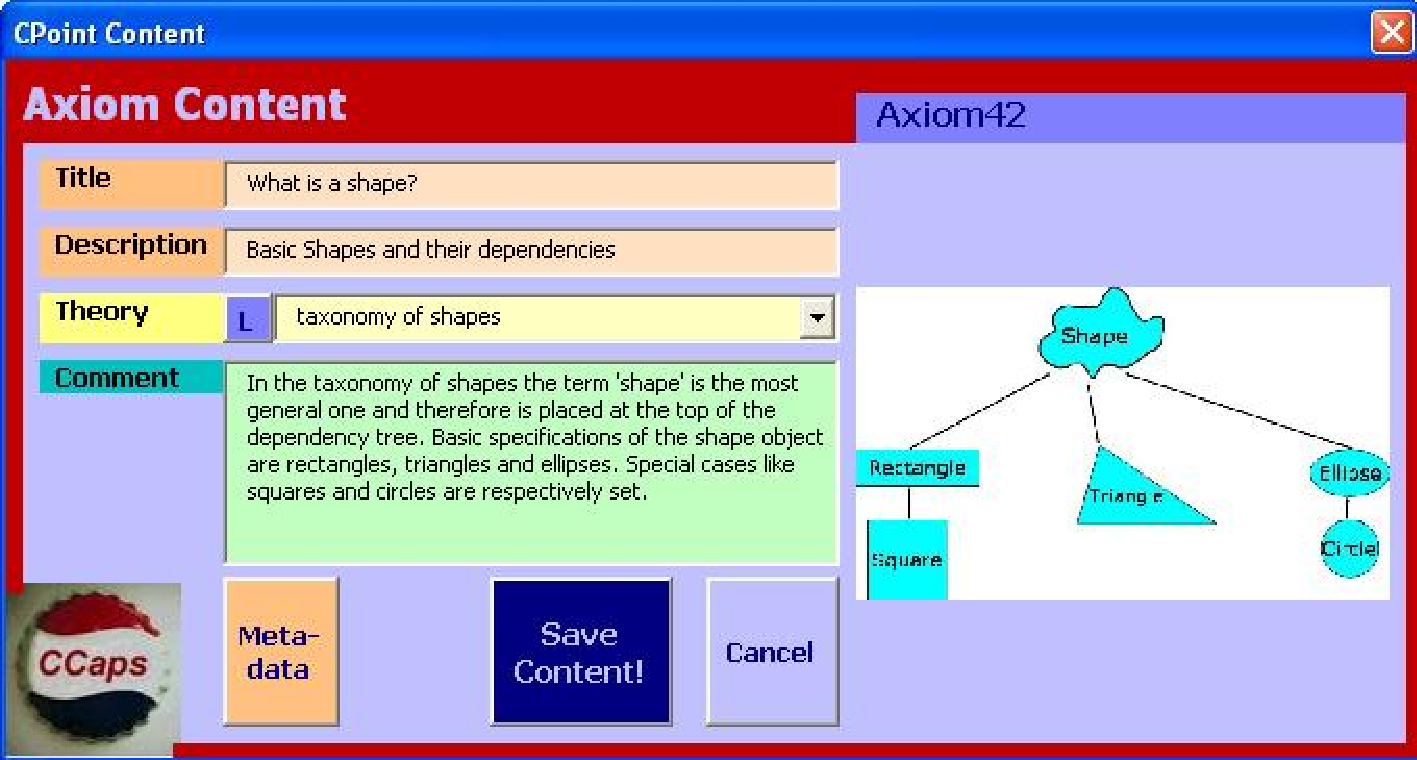
\includegraphics[width=9cm]{projects/cpoint/CPointContent}
\end{myfig}
The information annotated in these processes can be exploited for
added-value services.

\paragraph{{\omdoc} Conversion}\label{sec:omdocize} The heart of {\cpoint} is the
functionality for converting a fully ({\cpoint}-)edited presentation into a valid {\omdoc}
document.  This generated {\omdoc} document can for instance be read into
computer-supported education systems like {\activemath} (see~\cite{activemathAIEDJ01} and
{\mysecref{activemath}}).

\paragraph{Added-Value Services}\label{sec:auxiliaries}
As author support is essential for the motivation doing the semantic markup process,
{\cpoint} offers the following added-value services:
\begin{description}
\item[{\bf{Content Search and
      Navigation}\twin{content}{search}\twin{content}{navigation}}] {\cpoint}'s
  {\scsys{GoTo}} facility makes use of the additional semantic quality of {\ppt} objects
  by offering content search. For instance if an author remembers the existence of a
  definition of ``equivalence'' in some (older) {\ppt} presentation, she might look up all
  {\ppt} objects in a collection of several {\ppt} presentations that are categorized as
  ``Definition'' and whose title contain the word ``equivalence''. The author is offered a list
  of all these objects and by selecting one she is directed to the specific {\ppt} object.
\item[{\bf Dependency Graphs}\twin{dependency}{graph}] {\cpgraphs} enables the user to
  view graph based presentations of the annotated knowledge on distinct detail levels.
\item[{\bf Semantics-Induced Presentation}\twin{semantics-induced}{presentation}] The
  module {\cpauthor} offers the presentation of the underlying semantics. Whenever the
  author selects a {\ppt} object basic semantic information (like category, title, and
  main references) is presented to her. With {\cpoint}'s Visualize Mode semantic labels
  for annotated {\ppt} objects are generated.
\item[{\bf Creation of Pre-Categorized {\ppt} Objects}] Based on an individually designed
  CSS style sheet categorized, styled {\ppt} objects can be {\emph{created}} with
  {\cpauthor}. The layout is determined in the CSS file by the respective category (e.g.
  proposition) or superordinate classification (e.g. assertion, content, general).
\item[{\bf Math Glyphs in {\ppt}}\twin{mathematical}{glyph}] Based on the {\ppt} add-in
  {\texpoint}, the CMath functionalities empower an author to define individual symbol
  presentations. {\cpoint} introduces a mathematical user interface, which fully
  integrates mathematical symbols into PowerPoint presentations based on the semantics of
  the underlying objects rather than simply generating appropriate ink marks. For
  instance, the author might categorize a {\ppt} object as a symbol with the name 'reals'
  for the real numbers. The specific Unicode character to represent the real numbers can
  be declared with {\cpoint}. Subsequently, whenever the author writes the text
  '\verb|\reals|' and activates the math mode, then this sequence of characters is
  replaced by the previously declared presentation. The symbol presentation may also be
  given in {\LaTeX} form so that {\texpoint} can transform the {\LaTeX} code into {\ppt}
  glyphs. Note that this feature is not limited to math glyphs but can be used for handy
  abbreviations (macros) as well.
\item[{\bf Editorial Notes}\twin{editorial}{note}] Treating {\ppt} presentations as
  content documents requires more editing, therefore {\cpnotes} add editorial
  functionalities like grouped editorial notes and {\indextoo{navigation}} within these.
\item[{\bf {\omdoc} To {\ppt}}] The {\cpimport} module enables the import of {\omdoc}
  documents into the {\ppt} application. According to an individual underlying CSS style sheet {\ppt}
  objects in a newly created {\ppt} presentation are generated.
\item[{\bf ActiveMath}] Integrated development environment for ActiveMath content and
  specific ActiveMath book creation for a selected {\ppt} object.
\end{description}

\subsection{Future Work}
In the future the addition of other added-value services for users is planned. We want to
shift the focus from the authoring role to the recipient role of a {\ppt} presentation,
e.g. in form of a {\cpstudent} module in accordance with the {\cpauthor} module.
Furthermore, a new, more basic and therefore more user-friendly interface for {\cpoint}
novices will be implemented. This {\cpbasic} module will try to overcome the heavily
form-oriented format of {\cpoint}. In a next step the growing of a {\cpoint} user will be
supported by offering advanced {\cpoint} utilities that will extend {\cpbasic}.
Additionally, the success of ``social software'' under the Web 2.0 paradigm like ``social
bookmarking'' gives rise to the idea of a new personal and sharable {\ppt} objects
management where the predefined categories in {\cpoint} are replaced by ``social tags''.
Another {\cpoint} project is its extension for usage by teachers in school, which
usefulness has already been established in~\cite{Kohlhase:emPowerPoint}. The newest
project at the International University of Bremen is the implementation of a
{\cpoint}-like editor for MS Word.

%%% Local Variables: 
%%% mode: latex
%%% TeX-master: "../../omdoc"
%%% End: 

% LocalWords:  CPoint CPointAuthor CPointStudent CPointBasic CPointGraphs DiMeB
% LocalWords:  CPointImport CPointNotes TexPoint cpoint LGPL omgroup metadata
% LocalWords:  activemath GoTo CMath reals ActiveMath ActiveMath menubar

\end{projectdescription}

\begin{projectdescription}
  %%%%%%%%%%%%%%%%%%%%%%%%%%%%%%%%%%%%%%%%%%%%%%%%%%%%%%%%%%%%%%%%%%%%%%%%%
% This file is part of the LaTeX sources of the OMDoc 1.3 specifiation
% Copyright (c) 2006 Christoph Lange
% This work is licensed by the Creative Commons Share-Alike license
% see http://creativecommons.org/licenses/by-sa/2.5/ for details
\svnInfo $Id: main.tex 8453 2009-08-04 09:58:26Z kohlhase $
\svnKeyword $HeadURL: https://svn.omdoc.org/repos/omdoc/branches/omdoc-1.3/doc/spec/projects/swim/main.tex $
%%%%%%%%%%%%%%%%%%%%%%%%%%%%%%%%%%%%%%%%%%%%%%%%%%%%%%%%%%%%%%%%%%%%%%%%%

\section{{\swim} -- An OMDoc-based Semantic Wiki}
\begin{project}{swim}{http://kwarc.eecs.iu-bremen.de/projects/swim}
\pauthors{Christoph Lange\and Michael Kohlhase}
\pinstitute{Computer Science, International University Bremen}
\end{project}

{\swim} is a semantic wiki for collaboratively building, editing and browsing a
mathematical knowledge base of {\omdoc} theories. Our long-term objective is to develop a
software that facilitates the creation of a shared, public collection of mathematical
knowledge and serves work groups of mathematicians as a tool for collaborative development
of new theories.  Even though the work reported here was initially motivated by solving
the MKM author's dilemma~\cite{KohKoh:cdad04}, we contend that the new application area
MKM can also contribute to the development of semantic wikis.

Technically, {\swim} is based on the semantic wiki engine
\scsys{IkeWiki}~\cite{schaffert06:ikewiki}, which was chosen because of its
modular design, its rich semantic web infrastructure, its user assistance for
annotations, and its orientation towards
learning~\cite{schaffert06:learning-with-semantic-wikis}.

\subsection{Semantic Wikis}

A wiki~\cite{LeuCun01:wikiway} is a web server
application that allows users to browse, create, and edit hyperlinked pages in a web
browser, usually using a simple text syntax.  In contrast to most content management
systems, wiki pages are accessible via an URL containing their title.  A new page can be
created by linking from an existent page to the page to be created.  This link will then
lead to an edit form.  Usually, anyone is allowed to edit pages on a wiki, but access can
be restricted.  Other characteristics of wikis include permanent storage of old page
versions (with facilities to display differences between two versions and to restore a
certain version), notification about recent changes, and full-text search.

Semantic
wikis~\cite{voelkel06:semanticwikistateoftheart,TolPas06:wikis-semantic-hypermedia}
enhance wikis by Semantic Web technologies, such as {\rdf}~\cite{LasSwi:rdf99} or
ontologies.  Usually one page represents one concept from a real-world domain, which has a
type, possibly some metadata, and typed links to other concepts.  For example, a link from
a wiki page about ``Life, the Universe and Everything'' to another page about Douglas
Adams could be typed as ``is author of''.  In terms of {\rdf}, this can be expressed by the
following subject--predicate--object triple,

\[
(\mbox{``Douglas Adams''},\;\mbox{isAuthorOf},\;\mbox{``Life, the Universe and
Everything''})
\]

where the \textit{isAuthorOf} relation would be defined in an ontology.  These links are
usually displayed in a navigation box next to the page contents. Semantic wikis only deal
with wiki text, not with mathematics, though some allow to embed mathematical formulae as
presentational-only {\TeX}.

{\swim} encourages users to collaborate: Non-mathematicians can collaborate in creating a
``Wikipedia of mathematics'' by compiling the knowledge available so far, while scientists
can collaboratively develop new theories.  Users get an immediate reward for many of their
contributions: Once they specify the type of a page or relations of one page to another,
this information will be displayed in a box of navigation links.  We intend to make the
data created in {\swim} usable for external services by offering an export facility for
{\omdoc} documents and by integrating them into {\swim}.  Mathematicians developing
theories will be assisted to retain an overview of theory dependencies in order not to
break them.  Social software services will further utilize the semantic information
available from the theories and from tracking the user interaction log (``Who did what on
which page when?'').  User feedback to pages can be extended to social bookmarking, which
is ``the practice of saving bookmarks [of Internet resources] to a public web site and
`tagging' them with keywords.''~\cite{lomas05:social-bookmarking} The more users tag a
certain resource, the higher a social bookmarking service will rank it.

The enhancements of the data model semantic wikis bring along --- compared to traditional
wikis --- are already present in the {\omdoc} format, so that an {\omdoc}-based wiki only
needs to operationalize their underlying meaning. For example, typed links, which are
implemented via an extension to the wiki syntax in \scsys{Semantic
  MediaWiki}~\cite{voelkel06:semanticwikipedia} or editable through a separate editor in
\scsys{IkeWiki}~\cite{schaffert06:ikewiki}, are implemented by means of the \texttt{for}
attribute to {\omdoc}'s elements (e.g.\ \texttt{<example for="\#id-of-assertion">}).
{\swim} makes them editable easily and visualizes them adequately.  A semantic wiki
targeted at mathematics must ensure that dependencies between concepts are preserved.
Results in this area will be interesting for non-mathematical semantic wikis as well,
especially when they support higher levels of formalization such as ontologies.

\subsection{Design of {\swim}}

\subsubsection{Concepts and Relations}

The smallest unit that can be displayed, edited, linked to, or archived in a wiki is a
page. In a semantic wiki, it usually describes one {\emph{concept}}, including its
properties and its relations to other concepts.  While standalone {\omdoc} documents can
contain more than one theory, is is important to keep pages small in a wiki to improve the
effectivity of usage.  Furthermore, usual semantic wikis only store and display metadata
and typed links per page; {\swim} does too.\footnote{Semantic information will only be
  considered on the theory and statement levels of {\omdoc} --- directly or through
  reasoning in the case of transitive closures ---, not on the object level.}  Users are
strongly encouraged to define at most one theory per wiki page and to roll out
non-constitutive statements (see {\mysecref{statements-constitutive}}) to separate pages,
referencing their context theory.  As constitutive statements cannot exist without an
enclosing theory, but as, on the other hand, we want each wiki page to form a valid
document, we introduced a new element {\element[ns-elt=swim]{page}}, which can be a child
of an {\element{omdoc}} element and which has the same content model as a
{\element{theory}} element --- in particular, it can hold several theory-constitutive
statements and connect them to their context theory.
\begin{wrapfigure}{r}{8cm}
  \begin{tikzpicture}[scale=1.5,thin,font=\sffamily,>=triangle 60]
    \tikzstyle{concept}=[font=\sffamily\bfseries,draw,minimum height=3.5ex,rounded corners]
    \tikzstyle{every path}=[font=\small\sffamily];
    \node[concept] (t) at (0,1) {theory};
    \node[concept,dashed] (s) at (0,0) {\itshape statement};
    \node[concept] (d) at +(-158:2.0cm) {definition};
    \begin{scope}[shift={(d)}]% control point for e->d
      \coordinate (da) at +(-90:1.5cm);% relative to s, not to a!
    \end{scope}
    \node[concept] (a) at +(-120:1.5cm) {assertion};
    \begin{scope}[shift={(a)}]% control point for e->a
      \coordinate (aa) at +(-30:1cm);% relative to s, not to a!
    \end{scope}
    \node[concept] (p) at +(-60:1.5cm) {proof};
    \node[concept] (e) at +(-22:2.0cm) {example};
    \draw[->] (t.-60) .. controls +(-60:0.5cm) and +(-30:0.5cm) .. node[right]
    {imports} (t.east);
    \draw[->] (s) -- node[left] {context for} (t);
    \draw[-open triangle 60] (d) -- node[above] {is a} (s);
    \draw[-open triangle 60] (a) -- node[above left] {is a} (s);
    \draw[-open triangle 60] (p) -- node[above right] {is a} (s);
    \draw[-open triangle 60] (e) -- node[above] {is a} (s);
    \draw[->] (p) -- node[above] {proves} (a);
    \draw[->] (e) ..
    controls +(-120:1cm)
    and (aa) ..
    node[below left] {exemplifies} (a);
    \draw[->] (e) ..
    controls +(-90:1.5cm)
    and (da) ..
    node[below left] {exemplifies} (d);
  \end{tikzpicture}
  \caption{Subset of {\omdoc}'s system ontology}\vspace*{-.5cm}
\end{wrapfigure}
{\omdoc}'s system ontology has been partly coded in OWL-DL and imported to the wiki's {\rdf}
store, which is implemented using the Jena Semantic Web Framework for
Java~\cite{URL:jena:web}. Theories as well as statements of any type form concepts, and
the most important relations between those concepts are extracted from the {\omdoc} pages
on saving and then stored as {\rdf} triples.  These relations include:
\begin{itemize}
\item The import relation between theories
\item The relation of a statement to its context theory
\item The relation of an example to the statement it exemplifies
\item The relation of a proof to the assertion it proves
\end{itemize}
It is planned to also take relations given by user interaction into consideration, such as
``Who edited which page when?'', and to combine ontology-defined relations and user
relations.  For example, a metric estimating the {\emph{degree of difficulty}} of a page,
calculated by counting the questions on the discussion page, could be implemented.
Furthermore, the user can specify taxonomic relations, which cannot be stated explicitly
in {\omdoc}, such as (``all differentiable functions are continuous''), as annotations in
an ontology language like {\rdf} Schema or {\owl}.

\subsubsection{User Interface and Interaction Model}

Pages can be rendered to XHTML plus presentational MathML using the transformations
described in {\mychapref{transform-xsl}}. There is also a browsable source code view, which is
useful for documents that are not written in textbook style.

Not only will the user be able to navigate along the dependency graph, she will also be
able to {\emph{interact}} with the system: she will be asked whether she wants to explore
the theories required as dependencies in further detail.

Suppose that the user is currently reading the page containing the theory {\snippet{ring}}
from the elementary algebra example from {\mychapref{dg-elal}}. In this case the wiki will
not only display navigation links to the direct dependencies {\snippet{group}} and
{\snippet{monoid}}, but it will also provide unobtrusive buttons that allow the user to
give one of the commands in {\myfigref{gui-showdeps}}. Not only the last case will be
recorded --- the others are interesting as well for \emph{social bookmarking}.  For
example, if many users requested a theory $t$ to be explained, the system could default to
display not only the direct dependencies but also the level-two dependencies, for it seems
that $t$ is too difficult for only being explained shallowly.

\begin{myfig}{gui-showdeps}{The command buttons to navigate along the dependencies}
  \begin{minipage}{8cm}
\begin{description}
\item[{\bf{No, thanks!}}] ``{\emph{I already know group and monoid.}}''
\item[{\bf{Explain}}] ``{\emph{Please show me group and monoid, I want to learn about
      ring's prerequisites.}}'' --- group and monoid will be displayed.
\item[{\bf{Explore}}] ``{\emph{Please show me {\emph{all}} prerequisites for ring.}}'' ---
  group, monoid, and semigroup, are opened in separate windows or serialized into one
  page.
\item[{\bf{Suspend}}] ``{\emph{I want to know about group and monoid, but only later.}}''
  --- {\swim} keeps a notice in the user's profile that she wants to read group and monoid
  sometime.  Reminder links to suspended theories are shown on a separate navigation bar.
\end{description}
\end{minipage}\quad
\begin{minipage}{2.5cm}
  
\includegraphics[width=2.5cm]{projects/swim/gui-showdeps}
\end{minipage}
\end{myfig}

\subsubsection{Further work}

Further work on {\swim} will concentrate on integrating a lightweight
management of change process.  Second, while the wiki is yet a user-friendly
\emph{browser}, there is still a demand for assisting users to \emph{edit}
{\omdoc}.  To this end, the {\qmath} preprocessor (see {\mysecref{qmath}}) will
be integrated into {\swim}.  Mathematical objects entered as {\qmath} will be
kept in this syntax for display in the edit form, but they will be converted to
{\omdoc} for rendering for presentation and when pages are exported to another
application.

%%% Local Variables: 
%%% mode: stex
%%% TeX-master: "../../omdoc"
%%% End: 

% LocalWords:  matwebsearch Ioan Sucan nC dx dy dt runningex XPointer ns attr
% LocalWords:  mq anyorder xmlns domainofapplication bvar ci cn eq OAI API da
% LocalWords:  Lange CPoint wikis dateness parseable isAuthorOf MediaWiki omdoc
% LocalWords:  aa wiki's Wiki wiki IkeWiki JA hypermedia elt semithick pres dg
% LocalWords:  elal gui showdeps qmath stex metadata wiki's scheint mir kein zu
% LocalWords:  Gegensatz sein

\end{projectdescription}

\begin{projectdescription}
  %%%%%%%%%%%%%%%%%%%%%%%%%%%%%%%%%%%%%%%%%%%%%%%%%%%%%%%%%%%%%%%%%%%%%%%%%
% This file is part of the LaTeX sources of the OMDoc 1.3 specifiation
% Copyright (c) 2006 Peter Jansen
% This work is licensed by the Creative Commons Share-Alike license
% see http://creativecommons.org/licenses/by-sa/2.5/ for details
\svnInfo $Id: report.tex 8453 2009-08-04 09:58:26Z kohlhase $
\svnKeyword $HeadURL: https://svn.omdoc.org/repos/omdoc/branches/omdoc-1.3/doc/spec/projects/omdocmode/report.tex $
%%%%%%%%%%%%%%%%%%%%%%%%%%%%%%%%%%%%%%%%%%%%%%%%%%%%%%%%%%%%%%%%%%%%%%%%%

\section{An Emacs mode for editing OMDoc Documents}
\begin{project}{omdocmode}{http://www.cs.cmu.edu/~ccaps}
\pauthors{Peter Jansen}
\pinstitute{School of Computer Science, Carnegie Mellon University}
\end{project}

We describe an {\emacs} major mode for editing {\omdoc} documents, developed by the {\scsys{Course Capsules}}
project group at the CMU School of Computer Science.  This mode extends the {\emacs}
editor~\cite{Stallman:em02} with functionality intended to help visualize, edit, and
create documents written in {\omdoc} format.

The mode is part of the {\omdoc} distribution (see {\mysecref{distribution}}), it is
provided under the conditions specified in the Library Gnu Public License~\cite{LGPL}.

\subsection{Introduction}

The CCaps project has developed tools to convert legacy materials written in a variety of
formats ({\scsys{PowerPoint}}, {\mathematica}, etc.)  into the {\omdoc} format (see
{\mysecsref{cpoint}{nb2omdoc}}). In many cases the output generated by such tools needs to
be post-processed or otherwise modified.

To this end, a user must open the file, read and understand its contents and perform the
appropriate modifications.  Though an {\omdoc} document is a regular text file, most of
its content consists of markup, which is hard to read and tedious to type.  It is
therefore important to support the user with tools that make a document easier to read and
modify, either in the form of a separate editor, or as an extension of an existing editor.

One approach to this is to build a {\emph{visual {\omdoc} editor}}, which presents the
document in a form resembling conventional mathematical documents (i.e., without showing
the markup explicitly, and with appropriate formatting for mathematical formulae), and
offers the user functionality to modify or annotate its content.

While this is ideal for user understanding of document content, it presupposes
consistent syntactic correctness, makes it more difficult to inspect or change
markup directly, and may present challenges as to resolving user action
ambiguities.

We have taken this approach in the {\cpoint} and {\mathematica} add-ins (see
{\mysecsref{cpoint}{nb2omdoc}}). But we also wanted a tool that would maintain full
control of all the textual information, while offering support for readability and editing
functionality.  We chose for this tool to extend the {\emacs} editor~\cite{Stallman:em02},
which lends itself very well to this task (as well as being the editor for general use for
several of our group).

\subsection{{\omdoc} mode functionality}

We now look at the different categories of
functionality in slightly more detail.

\paragraph{Visualization}
is currently provided by the use of the {\emacs} {\emph{font-lock}} mechanism to give
different categories of tags and content different fonts and colors to make them easily
recognizable.  Element categories currently recognized correspond to the {\omdoc} 1.2
modules: Document structure, Math, Theories, Auxiliaries, Presentation, {\openmath}, and
the {\indextoo{Dublin Core}} elements.

A customizable {\emph{indentation function}} allows for intelligible layout, which is
helpful both in hand-coding and the editing of the output of a legacy transformation
process.  There are key bindings for line, region, and enclosing element indentation.

\paragraph{Editing}
Functionality consists mainly of automated insertion of {\emph{templates}} for each of the
{\omdoc} elements, both via mode-dependent menu options and key bindings, grouped by
element category (the same categories as given above).

The template insertion mechanism is based on {\snippet{tempo.el}}, which allows for the
maintenance of a {\emph{list of insertion points}} the user can navigate in between to
supply or change the values of certain attributes.

The main function currently available for completing incomplete elements is the equivalent
of the standard {\snippet{electric-/}} function.  We are planning to add several other
completion functions in the near future (for tags, tag sets, attribute names, and symbol
and theory names).

The mode also provides for {\emph{validation}}: either internally (as a simple local
syntax check to check well-formedness) or externally (via an external xml validation
validation engine).  Internal validation builds an abbreviated parse tree, and highlights
discrepancies, suggesting possible modifications of insertions of element opening or
closing tags.  External validation runs an external xml validation engine ({\rxp} or
{\nsgmls}, depending on the configuration variables), and shows the output in a separate
buffer.

\begin{myfig}{skeleton}{Opening a new Buffer in {\omdoc} Mode}
  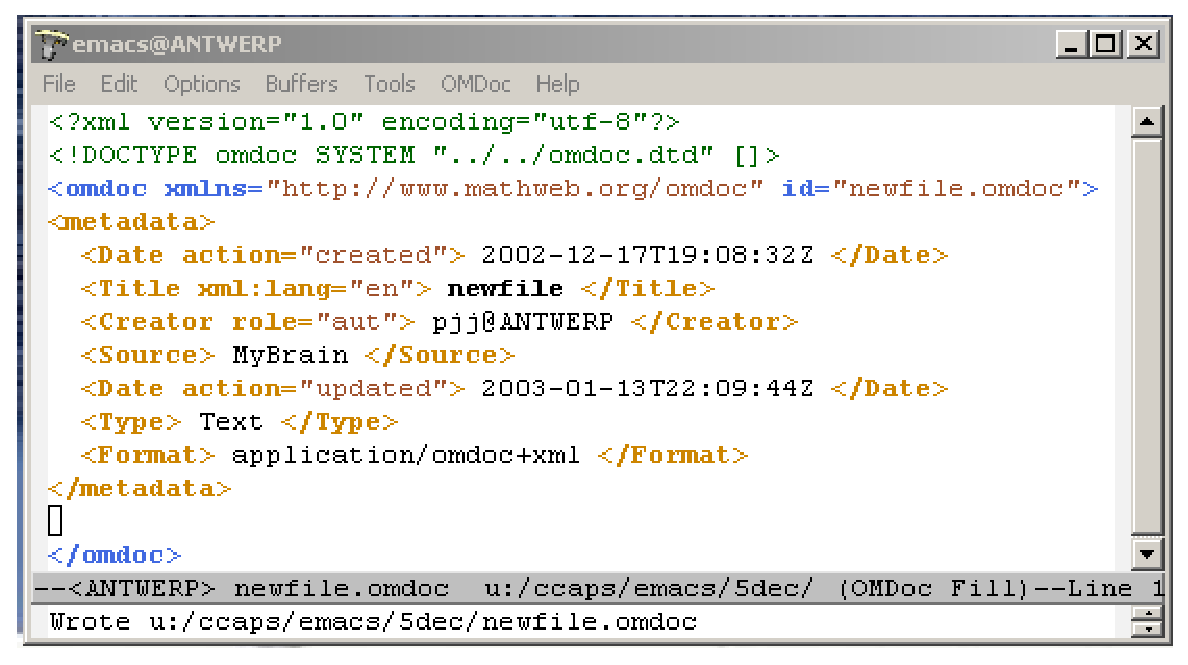
\includegraphics[width=9cm]{projects/omdocmode/omdoc2c}
\end{myfig}

\paragraph{Document creation}
is supported by automatic insertion of a basic {\emph{{\omdoc} skeleton}} in new buffers
as well as a {\emph{time-stamp updating}} mechanism and some smaller functions that extract
information from the user's environment variables to supply information for some of the
metadata slots (see the example in {\myfigref{skeleton}} below).

\subsection{Examples}

We illustrate some of the above by means of a few screen shots.  The example in
{\myfigref{menu}} is taken while editing a document that was semi-automatically generated
from part of a {\mathematica} notebook~(\cite{Sutner:cmnto04}).  Here, the user has
already run an automated indentation function, for example by activating
{\snippet{omdoc-indent-enclosing-main}} by typing {\snippet{C-c C-q}}, and is now about to
use the {\omdoc} menu to enter a new construct.


\begin{myfig}{menu}{Editing an {\omdoc} Document}
  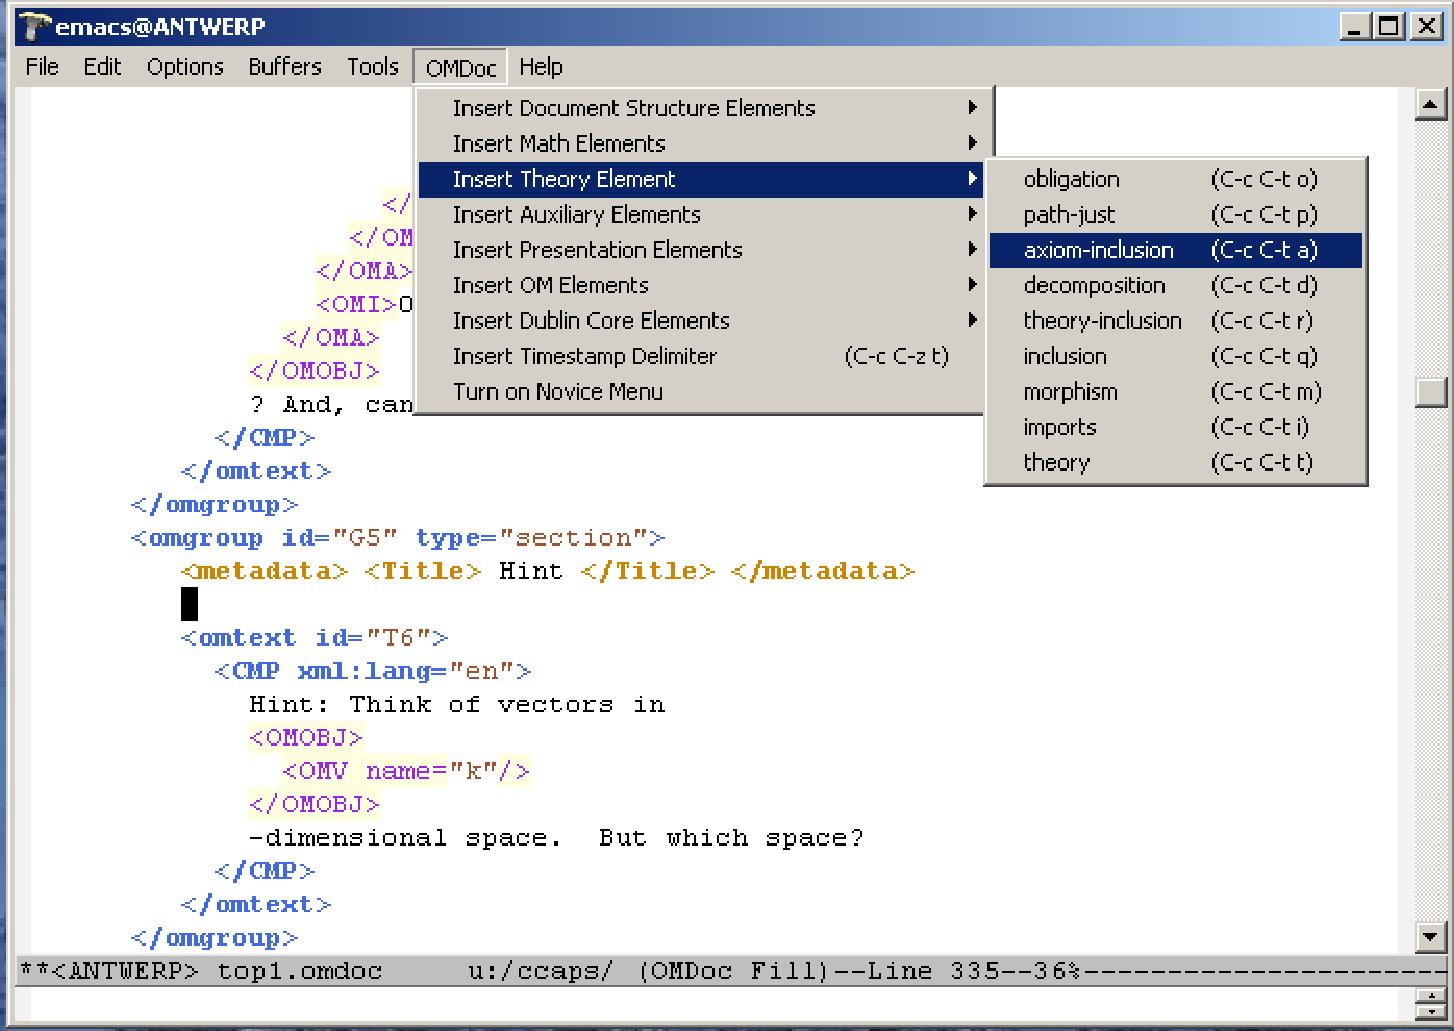
\includegraphics[width=9cm]{projects/omdocmode/omdoc1c}
\end{myfig}

After this operation, which could also have been performed by typing the key sequence
{\snippet{C-c C-t a}}), {\emacs} inserts the following text at the point (i.e. cursor
position).
\begin{lstlisting}
<axiom-inclusion xml:id="" to=""> </axiom-inclusion>
\end{lstlisting}

The second example shows the skeleton template that is automatically inserted when the
user opens a new file: {\myfigref{skeleton}}.  Note that the file name has been used as id
and title automatically, and the user's address appears in the Author field.  Timestamps
are inserted in Date fields for both creation and update, and the latter is adjusted
automatically every time changes are saved to the file.

%%% Local Variables: 
%%% mode: latex
%%% TeX-master: "../../omdoc"
%%% End: 

% LocalWords:  omdocmode el CCaps cpoint nb omdoc metadata

\end{projectdescription}

\begin{projectdescription}
  %%%%%%%%%%%%%%%%%%%%%%%%%%%%%%%%%%%%%%%%%%%%%%%%%%%%%%%%%%%%%%%%%%%%%%%%%
% This file is part of the LaTeX sources of the OMDoc 1.3 specifiation
% Copyright (c) 2006 Klaus Sutner
% This work is licensed by the Creative Commons Share-Alike license
% see http://creativecommons.org/licenses/by-sa/2.5/ for details
\svnInfo $Id: nb2omdoc.tex 8453 2009-08-04 09:58:26Z kohlhase $
\svnKeyword $HeadURL: https://svn.omdoc.org/repos/omdoc/branches/omdoc-1.3/doc/spec/projects/mathematica/nb2omdoc.tex $
%%%%%%%%%%%%%%%%%%%%%%%%%%%%%%%%%%%%%%%%%%%%%%%%%%%%%%%%%%%%%%%%%%%%%%%%%
\def\nb2om{\scsys{nb2omdoc}}

\section{Converting Mathematica Notebooks to OMDoc}
\begin{project}{nb2omdoc}{http://www.cs.cmu.edu/~ccaps}
\pauthors{Klaus Sutner}
\pinstitute{School of Computer Science, Carnegie Mellon University}
\end{project}

We describe a tool that converts {\mathematica} notebooks to {\omdoc}.  The program is
implemented entirely in {\mathematica} and easily extensible.

Creating an editor for general mathematical documents is notoriously difficult, in
particular when input methods are required that mimic the traditional two-dimensional
layout of many formulae.  Thus, it seems natural to use an existing high-quality system
such as the {\mathematica} notebook front end as an authoring tool for mathematical
documents.  A considerable amount of effort has gone into the design of this front end, see
for example~\cite{Wolfram00:mathnotation}, resulting in a surprisingly versatile system.
The notebook front end provides a rich set of palettes that allow inexperienced users to
construct complicated expressions almost instantaneously.  For more advanced users there
is a well-thought-out set of keyboard operations that make it possible to create, navigate
and edit two-dimensional expressions with relative ease and without recourse to
time-consuming mouse-based operations.  Unlike with {\TeX}, the results are immediately
visible and corrections are easy to make.  Nonetheless, the quality of the typeset
expression approaches that of {\TeX}.  Last, but not least, the {\mathematica} kernel can
be used to generate complicated expressions and even whole notebooks automatically.

{\mathematica} provides significant support for import, export and manipulation of {\xml}
documents and expressions, see~\cite{Wolfram.02}.  Thus, one can export a notebook in
{\mathml} format, or in a special {\scsys{NotebookML}} format.  Unfortunately, these
export mechanisms cannot be modified directly to produce highly marked-up documents in
{\omdoc} format.

The {\nb2om} converter uses a recursive descent parser, that scans the given notebook
document and generates corresponding {\omdoc}.  As far as structured text is concerned
this is a fairly straightforward operation.  However, special care needs to be taken to
deal with mathematical text elements, such as definitions, theorems, proofs and such like,
and mathematical expressions, in inline format as textual elements as well as in
evaluatable format (as input for the {\mathematica} kernel).  We comment on both issues in
turn.

{\mathematica} notebooks provide reasonable support for the creation of
well-structured documents, but enforce no particular discipline.  A fragment of a
typical notebook, showing some section headers and a bit of text with inline
mathematical formulae is shown in {\myfigref{autosrc}}.

\begin{myfig}{autosrc}{A {\mathematica} Notebook}
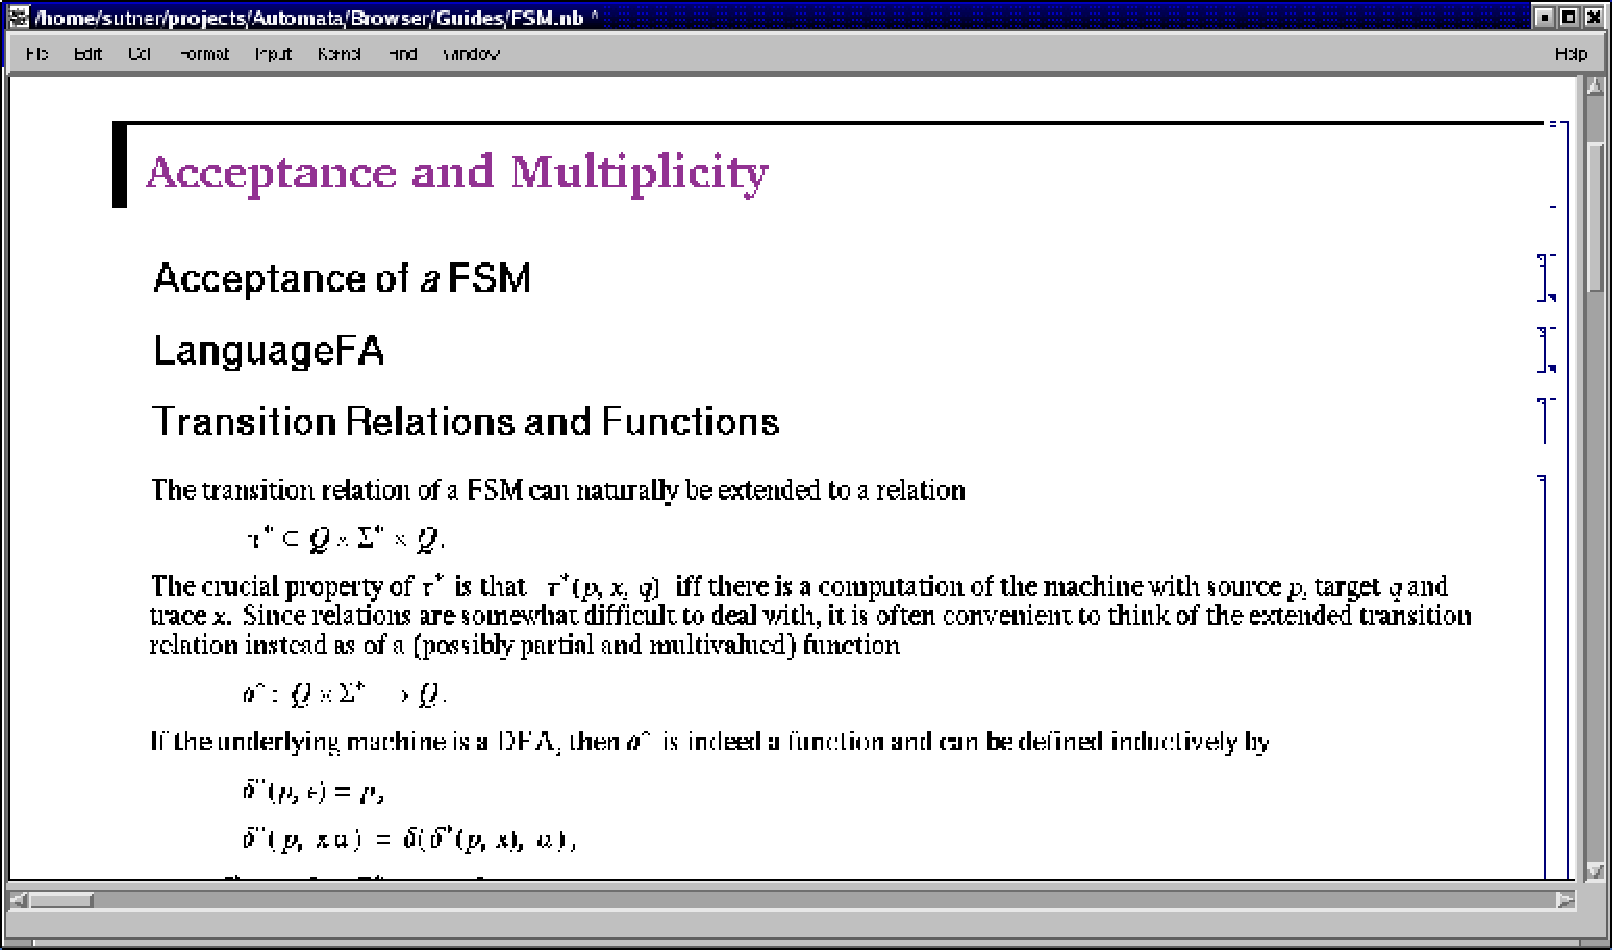
\includegraphics[width=10cm]{projects/mathematica/autosrc}
\end{myfig}

In order to facilitate the translation process it is advisable to front-load the
process: the author of the notebook is encouraged to use a special notebook
stylesheet, {\snippet{OMDocStyle.nb}}, that defines a number of syntactic categories
normally absent in a notebook.  These categories are implemented as a combination
of the cell types and cell labels.  As a typical example, consider a proof of some
assertion such as a theorem.  Ordinarily, a sequence of plain text cells would be
used to express a proof since none of the standard {\mathematica} stylesheets
provide a special proof style--though some have a theorem style.  The elements
defined in {\snippet{OMDocStyle.nb}} are easily accessible via pulldown menus or via
keyboard shortcuts in the notebook front end.  Moreover, the special styles are
color-coded in the notebook, so that it is easy for the author to see which
elements are present and which might be missing.


The conversion of mathematical expressions in the notebook is accomplished in a two-step
procedure.  First, we use the built-in {\mathematica} operation
{\snippet{ExpressionToSymbolicMathML}} that produces a symbolic expression representing a
MathML term that corresponds to the original notebook expression.  In a second,
post-processing step this expression is then transformed into an {\openmath} expression.
The post-processing relies heavily on the sophisticated pattern matching mechanism in
{\mathematica} and uses a special collection of rewrite rules.  The rules are based on
fairly simple-minded heuristics but do produce adequate results so long as the starting
expression is not too complicated.  As an example, consider the simple polynomial
expression $a x^2 + b x + c$ whose internal representation in {\mathematica} looks like so
(we assume here the expression appears inline within a block of text, the situation for an
input expression is entirely similar):
\begin{lstlisting}
Cell[ BoxData[FormBox[RowBox[{ 
      RowBox[{"a", " ", SuperscriptBox["x", "2"]}], "+", " ", 
      RowBox[{"b", " ", "x"}], " ", "+", " ", "c"}], 
        TraditionalForm]]]
\end{lstlisting}
The first conversion step produces the following {\mathematica} expression, 
shortened here to save space:
\begin{lstlisting}
XMLElement["math", 
  {"xmlns" ->"http://www.w3.org/1998/Math/MathML"}, 
  {XMLElement[ "apply", {}, {XMLElement["plus", {}, {}], 
   XMLElement[ "apply", {}, {XMLElement["times", {}, {}], 
     XMLElement["ci", {}, {"a"}], 
     XMLElement[ "apply", {}, {XMLElement["power", {}, {}], 
       XMLElement["ci", {}, {"x"}], 
       XMLElement["cn", {"type"->"integer"}, {"2"}]}]}], ...  }]}]
\end{lstlisting}
The post-processing finally yields the 
following expression, again shown only in part. 
\begin{lstlisting}
XMLElement["OMOBJ", {}, {XMLElement["OMA", {}, 
     {XMLElement["OMS", 
           {"cd"->"arith1", "name"->"plus"}, {}],
        XMLElement["OMA", {}, {XMLElement[ "OMS", 
           {"cd"->"arith1", "name"->"times"}, {}], 
        XMLElement["OMV", {"name"->"a"}, {}], 
        XMLElement["OMA", {}, {XMLElement["OMS", 
           {"cd"->"arith1", "name"->"power"}, {}], ...}]}]}]}]
\end{lstlisting}

The content dictionary was properly guessed in this instance.  Judging from the limited
experiments we have undertaken so far, it seems reasonable to expect that a fair amount of
the translation can be automated given that the field of discourse is limited, and that
the author is willing to customize the rewrite rules that control the post-processing
step.  Fortuitously, very little knowledge of {\mathematica} programming beyond some basic
syntax is necessary for the creation of these rules; mathematicians are likely to find
these rules fairly intuitive and natural.

At present, the conversion program is somewhat limited in its ability to deal with
arbitrarily structured notebooks.  It works well with a suite of notebooks developed
specifically for the {\snippet{OMDocStyle.nb}}, but requires modification for other types
of notebooks.  While it is not our goal to provide a truly general conversion tool with a
scope comparable to, say, the built-in conversion to MathML, some generalizations are
still needed at this point.

Another crucial issue is the extension of the rewrite rules used in the post-processing
step leading from MathML to {\openmath}.  No effort has been made so far to systematically
generate a set of rules suitable for a large class of documents.  At the very least, an
extension mechanism is needed that makes it easy for non-expert users to create the
necessary rule tables.

Lastly, it is desirable to create a {\mathematica} palette-based tool that focuses
more narrowly on the authoring and conversion of mathematical expressions only
rather than whole notebooks.  The generated raw {\openmath} expressions can be fed
directly into a low-level editor such as {\scsys{emacs}} using the special {\omdoc} mode
created as part of the {\ccaps} project, see elsewhere in this volume for a
description.

% LocalWords:  NotebookML evaluatable stylesheet OMDocStyle stylesheets BoxData
% LocalWords:  pulldown ExpressionToSymbolicMathML OpenMath FormBox RowBox nb
% LocalWords:  SuperscriptBox TraditionalForm XMLElement xmlns OMOBJ omdoc ci
% LocalWords:  arith CCaps thebib Sutner autosrc cn OMA cd OMV emacs

%%% Local Variables: 
%%% mode: latex
%%% TeX-master: "../../omdoc"
%%% End: 

\end{projectdescription}

\begin{projectdescription}
  %%%%%%%%%%%%%%%%%%%%%%%%%%%%%%%%%%%%%%%%%%%%%%%%%%%%%%%%%%%%%%%%%%%%%%%%%
% This file is part of the LaTeX sources of the OMDoc 1.3 specifiation
% Copyright (c) 2006 Christoph Lange
% This work is licensed by the Creative Commons Share-Alike license
% see http://creativecommons.org/licenses/by-sa/2.5/ for details
\svnInfo $Id: main.tex 8453 2009-08-04 09:58:26Z kohlhase $
\svnKeyword $HeadURL: https://svn.omdoc.org/repos/omdoc/branches/omdoc-1.3/doc/spec/projects/swim/main.tex $
%%%%%%%%%%%%%%%%%%%%%%%%%%%%%%%%%%%%%%%%%%%%%%%%%%%%%%%%%%%%%%%%%%%%%%%%%

\section{{\swim} -- An OMDoc-based Semantic Wiki}
\begin{project}{swim}{http://kwarc.eecs.iu-bremen.de/projects/swim}
\pauthors{Christoph Lange\and Michael Kohlhase}
\pinstitute{Computer Science, International University Bremen}
\end{project}

{\swim} is a semantic wiki for collaboratively building, editing and browsing a
mathematical knowledge base of {\omdoc} theories. Our long-term objective is to develop a
software that facilitates the creation of a shared, public collection of mathematical
knowledge and serves work groups of mathematicians as a tool for collaborative development
of new theories.  Even though the work reported here was initially motivated by solving
the MKM author's dilemma~\cite{KohKoh:cdad04}, we contend that the new application area
MKM can also contribute to the development of semantic wikis.

Technically, {\swim} is based on the semantic wiki engine
\scsys{IkeWiki}~\cite{schaffert06:ikewiki}, which was chosen because of its
modular design, its rich semantic web infrastructure, its user assistance for
annotations, and its orientation towards
learning~\cite{schaffert06:learning-with-semantic-wikis}.

\subsection{Semantic Wikis}

A wiki~\cite{LeuCun01:wikiway} is a web server
application that allows users to browse, create, and edit hyperlinked pages in a web
browser, usually using a simple text syntax.  In contrast to most content management
systems, wiki pages are accessible via an URL containing their title.  A new page can be
created by linking from an existent page to the page to be created.  This link will then
lead to an edit form.  Usually, anyone is allowed to edit pages on a wiki, but access can
be restricted.  Other characteristics of wikis include permanent storage of old page
versions (with facilities to display differences between two versions and to restore a
certain version), notification about recent changes, and full-text search.

Semantic
wikis~\cite{voelkel06:semanticwikistateoftheart,TolPas06:wikis-semantic-hypermedia}
enhance wikis by Semantic Web technologies, such as {\rdf}~\cite{LasSwi:rdf99} or
ontologies.  Usually one page represents one concept from a real-world domain, which has a
type, possibly some metadata, and typed links to other concepts.  For example, a link from
a wiki page about ``Life, the Universe and Everything'' to another page about Douglas
Adams could be typed as ``is author of''.  In terms of {\rdf}, this can be expressed by the
following subject--predicate--object triple,

\[
(\mbox{``Douglas Adams''},\;\mbox{isAuthorOf},\;\mbox{``Life, the Universe and
Everything''})
\]

where the \textit{isAuthorOf} relation would be defined in an ontology.  These links are
usually displayed in a navigation box next to the page contents. Semantic wikis only deal
with wiki text, not with mathematics, though some allow to embed mathematical formulae as
presentational-only {\TeX}.

{\swim} encourages users to collaborate: Non-mathematicians can collaborate in creating a
``Wikipedia of mathematics'' by compiling the knowledge available so far, while scientists
can collaboratively develop new theories.  Users get an immediate reward for many of their
contributions: Once they specify the type of a page or relations of one page to another,
this information will be displayed in a box of navigation links.  We intend to make the
data created in {\swim} usable for external services by offering an export facility for
{\omdoc} documents and by integrating them into {\swim}.  Mathematicians developing
theories will be assisted to retain an overview of theory dependencies in order not to
break them.  Social software services will further utilize the semantic information
available from the theories and from tracking the user interaction log (``Who did what on
which page when?'').  User feedback to pages can be extended to social bookmarking, which
is ``the practice of saving bookmarks [of Internet resources] to a public web site and
`tagging' them with keywords.''~\cite{lomas05:social-bookmarking} The more users tag a
certain resource, the higher a social bookmarking service will rank it.

The enhancements of the data model semantic wikis bring along --- compared to traditional
wikis --- are already present in the {\omdoc} format, so that an {\omdoc}-based wiki only
needs to operationalize their underlying meaning. For example, typed links, which are
implemented via an extension to the wiki syntax in \scsys{Semantic
  MediaWiki}~\cite{voelkel06:semanticwikipedia} or editable through a separate editor in
\scsys{IkeWiki}~\cite{schaffert06:ikewiki}, are implemented by means of the \texttt{for}
attribute to {\omdoc}'s elements (e.g.\ \texttt{<example for="\#id-of-assertion">}).
{\swim} makes them editable easily and visualizes them adequately.  A semantic wiki
targeted at mathematics must ensure that dependencies between concepts are preserved.
Results in this area will be interesting for non-mathematical semantic wikis as well,
especially when they support higher levels of formalization such as ontologies.

\subsection{Design of {\swim}}

\subsubsection{Concepts and Relations}

The smallest unit that can be displayed, edited, linked to, or archived in a wiki is a
page. In a semantic wiki, it usually describes one {\emph{concept}}, including its
properties and its relations to other concepts.  While standalone {\omdoc} documents can
contain more than one theory, is is important to keep pages small in a wiki to improve the
effectivity of usage.  Furthermore, usual semantic wikis only store and display metadata
and typed links per page; {\swim} does too.\footnote{Semantic information will only be
  considered on the theory and statement levels of {\omdoc} --- directly or through
  reasoning in the case of transitive closures ---, not on the object level.}  Users are
strongly encouraged to define at most one theory per wiki page and to roll out
non-constitutive statements (see {\mysecref{statements-constitutive}}) to separate pages,
referencing their context theory.  As constitutive statements cannot exist without an
enclosing theory, but as, on the other hand, we want each wiki page to form a valid
document, we introduced a new element {\element[ns-elt=swim]{page}}, which can be a child
of an {\element{omdoc}} element and which has the same content model as a
{\element{theory}} element --- in particular, it can hold several theory-constitutive
statements and connect them to their context theory.
\begin{wrapfigure}{r}{8cm}
  \begin{tikzpicture}[scale=1.5,thin,font=\sffamily,>=triangle 60]
    \tikzstyle{concept}=[font=\sffamily\bfseries,draw,minimum height=3.5ex,rounded corners]
    \tikzstyle{every path}=[font=\small\sffamily];
    \node[concept] (t) at (0,1) {theory};
    \node[concept,dashed] (s) at (0,0) {\itshape statement};
    \node[concept] (d) at +(-158:2.0cm) {definition};
    \begin{scope}[shift={(d)}]% control point for e->d
      \coordinate (da) at +(-90:1.5cm);% relative to s, not to a!
    \end{scope}
    \node[concept] (a) at +(-120:1.5cm) {assertion};
    \begin{scope}[shift={(a)}]% control point for e->a
      \coordinate (aa) at +(-30:1cm);% relative to s, not to a!
    \end{scope}
    \node[concept] (p) at +(-60:1.5cm) {proof};
    \node[concept] (e) at +(-22:2.0cm) {example};
    \draw[->] (t.-60) .. controls +(-60:0.5cm) and +(-30:0.5cm) .. node[right]
    {imports} (t.east);
    \draw[->] (s) -- node[left] {context for} (t);
    \draw[-open triangle 60] (d) -- node[above] {is a} (s);
    \draw[-open triangle 60] (a) -- node[above left] {is a} (s);
    \draw[-open triangle 60] (p) -- node[above right] {is a} (s);
    \draw[-open triangle 60] (e) -- node[above] {is a} (s);
    \draw[->] (p) -- node[above] {proves} (a);
    \draw[->] (e) ..
    controls +(-120:1cm)
    and (aa) ..
    node[below left] {exemplifies} (a);
    \draw[->] (e) ..
    controls +(-90:1.5cm)
    and (da) ..
    node[below left] {exemplifies} (d);
  \end{tikzpicture}
  \caption{Subset of {\omdoc}'s system ontology}\vspace*{-.5cm}
\end{wrapfigure}
{\omdoc}'s system ontology has been partly coded in OWL-DL and imported to the wiki's {\rdf}
store, which is implemented using the Jena Semantic Web Framework for
Java~\cite{URL:jena:web}. Theories as well as statements of any type form concepts, and
the most important relations between those concepts are extracted from the {\omdoc} pages
on saving and then stored as {\rdf} triples.  These relations include:
\begin{itemize}
\item The import relation between theories
\item The relation of a statement to its context theory
\item The relation of an example to the statement it exemplifies
\item The relation of a proof to the assertion it proves
\end{itemize}
It is planned to also take relations given by user interaction into consideration, such as
``Who edited which page when?'', and to combine ontology-defined relations and user
relations.  For example, a metric estimating the {\emph{degree of difficulty}} of a page,
calculated by counting the questions on the discussion page, could be implemented.
Furthermore, the user can specify taxonomic relations, which cannot be stated explicitly
in {\omdoc}, such as (``all differentiable functions are continuous''), as annotations in
an ontology language like {\rdf} Schema or {\owl}.

\subsubsection{User Interface and Interaction Model}

Pages can be rendered to XHTML plus presentational MathML using the transformations
described in {\mychapref{transform-xsl}}. There is also a browsable source code view, which is
useful for documents that are not written in textbook style.

Not only will the user be able to navigate along the dependency graph, she will also be
able to {\emph{interact}} with the system: she will be asked whether she wants to explore
the theories required as dependencies in further detail.

Suppose that the user is currently reading the page containing the theory {\snippet{ring}}
from the elementary algebra example from {\mychapref{dg-elal}}. In this case the wiki will
not only display navigation links to the direct dependencies {\snippet{group}} and
{\snippet{monoid}}, but it will also provide unobtrusive buttons that allow the user to
give one of the commands in {\myfigref{gui-showdeps}}. Not only the last case will be
recorded --- the others are interesting as well for \emph{social bookmarking}.  For
example, if many users requested a theory $t$ to be explained, the system could default to
display not only the direct dependencies but also the level-two dependencies, for it seems
that $t$ is too difficult for only being explained shallowly.

\begin{myfig}{gui-showdeps}{The command buttons to navigate along the dependencies}
  \begin{minipage}{8cm}
\begin{description}
\item[{\bf{No, thanks!}}] ``{\emph{I already know group and monoid.}}''
\item[{\bf{Explain}}] ``{\emph{Please show me group and monoid, I want to learn about
      ring's prerequisites.}}'' --- group and monoid will be displayed.
\item[{\bf{Explore}}] ``{\emph{Please show me {\emph{all}} prerequisites for ring.}}'' ---
  group, monoid, and semigroup, are opened in separate windows or serialized into one
  page.
\item[{\bf{Suspend}}] ``{\emph{I want to know about group and monoid, but only later.}}''
  --- {\swim} keeps a notice in the user's profile that she wants to read group and monoid
  sometime.  Reminder links to suspended theories are shown on a separate navigation bar.
\end{description}
\end{minipage}\quad
\begin{minipage}{2.5cm}
  
\includegraphics[width=2.5cm]{projects/swim/gui-showdeps}
\end{minipage}
\end{myfig}

\subsubsection{Further work}

Further work on {\swim} will concentrate on integrating a lightweight
management of change process.  Second, while the wiki is yet a user-friendly
\emph{browser}, there is still a demand for assisting users to \emph{edit}
{\omdoc}.  To this end, the {\qmath} preprocessor (see {\mysecref{qmath}}) will
be integrated into {\swim}.  Mathematical objects entered as {\qmath} will be
kept in this syntax for display in the edit form, but they will be converted to
{\omdoc} for rendering for presentation and when pages are exported to another
application.

%%% Local Variables: 
%%% mode: stex
%%% TeX-master: "../../omdoc"
%%% End: 

% LocalWords:  matwebsearch Ioan Sucan nC dx dy dt runningex XPointer ns attr
% LocalWords:  mq anyorder xmlns domainofapplication bvar ci cn eq OAI API da
% LocalWords:  Lange CPoint wikis dateness parseable isAuthorOf MediaWiki omdoc
% LocalWords:  aa wiki's Wiki wiki IkeWiki JA hypermedia elt semithick pres dg
% LocalWords:  elal gui showdeps qmath stex metadata wiki's scheint mir kein zu
% LocalWords:  Gegensatz sein

\end{projectdescription}

\begin{projectdescription}
  %%%%%%%%%%%%%%%%%%%%%%%%%%%%%%%%%%%%%%%%%%%%%%%%%%%%%%%%%%%%%%%%%%%%%%%%%
% This file is part of the LaTeX sources of the OMDoc 1.3 specifiation
% Copyright (c) 2006 Christoph Lange
% This work is licensed by the Creative Commons Share-Alike license
% see http://creativecommons.org/licenses/by-sa/2.5/ for details
\svnInfo $Id: main.tex 8453 2009-08-04 09:58:26Z kohlhase $
\svnKeyword $HeadURL: https://svn.omdoc.org/repos/omdoc/branches/omdoc-1.3/doc/spec/projects/swim/main.tex $
%%%%%%%%%%%%%%%%%%%%%%%%%%%%%%%%%%%%%%%%%%%%%%%%%%%%%%%%%%%%%%%%%%%%%%%%%

\section{{\swim} -- An OMDoc-based Semantic Wiki}
\begin{project}{swim}{http://kwarc.eecs.iu-bremen.de/projects/swim}
\pauthors{Christoph Lange\and Michael Kohlhase}
\pinstitute{Computer Science, International University Bremen}
\end{project}

{\swim} is a semantic wiki for collaboratively building, editing and browsing a
mathematical knowledge base of {\omdoc} theories. Our long-term objective is to develop a
software that facilitates the creation of a shared, public collection of mathematical
knowledge and serves work groups of mathematicians as a tool for collaborative development
of new theories.  Even though the work reported here was initially motivated by solving
the MKM author's dilemma~\cite{KohKoh:cdad04}, we contend that the new application area
MKM can also contribute to the development of semantic wikis.

Technically, {\swim} is based on the semantic wiki engine
\scsys{IkeWiki}~\cite{schaffert06:ikewiki}, which was chosen because of its
modular design, its rich semantic web infrastructure, its user assistance for
annotations, and its orientation towards
learning~\cite{schaffert06:learning-with-semantic-wikis}.

\subsection{Semantic Wikis}

A wiki~\cite{LeuCun01:wikiway} is a web server
application that allows users to browse, create, and edit hyperlinked pages in a web
browser, usually using a simple text syntax.  In contrast to most content management
systems, wiki pages are accessible via an URL containing their title.  A new page can be
created by linking from an existent page to the page to be created.  This link will then
lead to an edit form.  Usually, anyone is allowed to edit pages on a wiki, but access can
be restricted.  Other characteristics of wikis include permanent storage of old page
versions (with facilities to display differences between two versions and to restore a
certain version), notification about recent changes, and full-text search.

Semantic
wikis~\cite{voelkel06:semanticwikistateoftheart,TolPas06:wikis-semantic-hypermedia}
enhance wikis by Semantic Web technologies, such as {\rdf}~\cite{LasSwi:rdf99} or
ontologies.  Usually one page represents one concept from a real-world domain, which has a
type, possibly some metadata, and typed links to other concepts.  For example, a link from
a wiki page about ``Life, the Universe and Everything'' to another page about Douglas
Adams could be typed as ``is author of''.  In terms of {\rdf}, this can be expressed by the
following subject--predicate--object triple,

\[
(\mbox{``Douglas Adams''},\;\mbox{isAuthorOf},\;\mbox{``Life, the Universe and
Everything''})
\]

where the \textit{isAuthorOf} relation would be defined in an ontology.  These links are
usually displayed in a navigation box next to the page contents. Semantic wikis only deal
with wiki text, not with mathematics, though some allow to embed mathematical formulae as
presentational-only {\TeX}.

{\swim} encourages users to collaborate: Non-mathematicians can collaborate in creating a
``Wikipedia of mathematics'' by compiling the knowledge available so far, while scientists
can collaboratively develop new theories.  Users get an immediate reward for many of their
contributions: Once they specify the type of a page or relations of one page to another,
this information will be displayed in a box of navigation links.  We intend to make the
data created in {\swim} usable for external services by offering an export facility for
{\omdoc} documents and by integrating them into {\swim}.  Mathematicians developing
theories will be assisted to retain an overview of theory dependencies in order not to
break them.  Social software services will further utilize the semantic information
available from the theories and from tracking the user interaction log (``Who did what on
which page when?'').  User feedback to pages can be extended to social bookmarking, which
is ``the practice of saving bookmarks [of Internet resources] to a public web site and
`tagging' them with keywords.''~\cite{lomas05:social-bookmarking} The more users tag a
certain resource, the higher a social bookmarking service will rank it.

The enhancements of the data model semantic wikis bring along --- compared to traditional
wikis --- are already present in the {\omdoc} format, so that an {\omdoc}-based wiki only
needs to operationalize their underlying meaning. For example, typed links, which are
implemented via an extension to the wiki syntax in \scsys{Semantic
  MediaWiki}~\cite{voelkel06:semanticwikipedia} or editable through a separate editor in
\scsys{IkeWiki}~\cite{schaffert06:ikewiki}, are implemented by means of the \texttt{for}
attribute to {\omdoc}'s elements (e.g.\ \texttt{<example for="\#id-of-assertion">}).
{\swim} makes them editable easily and visualizes them adequately.  A semantic wiki
targeted at mathematics must ensure that dependencies between concepts are preserved.
Results in this area will be interesting for non-mathematical semantic wikis as well,
especially when they support higher levels of formalization such as ontologies.

\subsection{Design of {\swim}}

\subsubsection{Concepts and Relations}

The smallest unit that can be displayed, edited, linked to, or archived in a wiki is a
page. In a semantic wiki, it usually describes one {\emph{concept}}, including its
properties and its relations to other concepts.  While standalone {\omdoc} documents can
contain more than one theory, is is important to keep pages small in a wiki to improve the
effectivity of usage.  Furthermore, usual semantic wikis only store and display metadata
and typed links per page; {\swim} does too.\footnote{Semantic information will only be
  considered on the theory and statement levels of {\omdoc} --- directly or through
  reasoning in the case of transitive closures ---, not on the object level.}  Users are
strongly encouraged to define at most one theory per wiki page and to roll out
non-constitutive statements (see {\mysecref{statements-constitutive}}) to separate pages,
referencing their context theory.  As constitutive statements cannot exist without an
enclosing theory, but as, on the other hand, we want each wiki page to form a valid
document, we introduced a new element {\element[ns-elt=swim]{page}}, which can be a child
of an {\element{omdoc}} element and which has the same content model as a
{\element{theory}} element --- in particular, it can hold several theory-constitutive
statements and connect them to their context theory.
\begin{wrapfigure}{r}{8cm}
  \begin{tikzpicture}[scale=1.5,thin,font=\sffamily,>=triangle 60]
    \tikzstyle{concept}=[font=\sffamily\bfseries,draw,minimum height=3.5ex,rounded corners]
    \tikzstyle{every path}=[font=\small\sffamily];
    \node[concept] (t) at (0,1) {theory};
    \node[concept,dashed] (s) at (0,0) {\itshape statement};
    \node[concept] (d) at +(-158:2.0cm) {definition};
    \begin{scope}[shift={(d)}]% control point for e->d
      \coordinate (da) at +(-90:1.5cm);% relative to s, not to a!
    \end{scope}
    \node[concept] (a) at +(-120:1.5cm) {assertion};
    \begin{scope}[shift={(a)}]% control point for e->a
      \coordinate (aa) at +(-30:1cm);% relative to s, not to a!
    \end{scope}
    \node[concept] (p) at +(-60:1.5cm) {proof};
    \node[concept] (e) at +(-22:2.0cm) {example};
    \draw[->] (t.-60) .. controls +(-60:0.5cm) and +(-30:0.5cm) .. node[right]
    {imports} (t.east);
    \draw[->] (s) -- node[left] {context for} (t);
    \draw[-open triangle 60] (d) -- node[above] {is a} (s);
    \draw[-open triangle 60] (a) -- node[above left] {is a} (s);
    \draw[-open triangle 60] (p) -- node[above right] {is a} (s);
    \draw[-open triangle 60] (e) -- node[above] {is a} (s);
    \draw[->] (p) -- node[above] {proves} (a);
    \draw[->] (e) ..
    controls +(-120:1cm)
    and (aa) ..
    node[below left] {exemplifies} (a);
    \draw[->] (e) ..
    controls +(-90:1.5cm)
    and (da) ..
    node[below left] {exemplifies} (d);
  \end{tikzpicture}
  \caption{Subset of {\omdoc}'s system ontology}\vspace*{-.5cm}
\end{wrapfigure}
{\omdoc}'s system ontology has been partly coded in OWL-DL and imported to the wiki's {\rdf}
store, which is implemented using the Jena Semantic Web Framework for
Java~\cite{URL:jena:web}. Theories as well as statements of any type form concepts, and
the most important relations between those concepts are extracted from the {\omdoc} pages
on saving and then stored as {\rdf} triples.  These relations include:
\begin{itemize}
\item The import relation between theories
\item The relation of a statement to its context theory
\item The relation of an example to the statement it exemplifies
\item The relation of a proof to the assertion it proves
\end{itemize}
It is planned to also take relations given by user interaction into consideration, such as
``Who edited which page when?'', and to combine ontology-defined relations and user
relations.  For example, a metric estimating the {\emph{degree of difficulty}} of a page,
calculated by counting the questions on the discussion page, could be implemented.
Furthermore, the user can specify taxonomic relations, which cannot be stated explicitly
in {\omdoc}, such as (``all differentiable functions are continuous''), as annotations in
an ontology language like {\rdf} Schema or {\owl}.

\subsubsection{User Interface and Interaction Model}

Pages can be rendered to XHTML plus presentational MathML using the transformations
described in {\mychapref{transform-xsl}}. There is also a browsable source code view, which is
useful for documents that are not written in textbook style.

Not only will the user be able to navigate along the dependency graph, she will also be
able to {\emph{interact}} with the system: she will be asked whether she wants to explore
the theories required as dependencies in further detail.

Suppose that the user is currently reading the page containing the theory {\snippet{ring}}
from the elementary algebra example from {\mychapref{dg-elal}}. In this case the wiki will
not only display navigation links to the direct dependencies {\snippet{group}} and
{\snippet{monoid}}, but it will also provide unobtrusive buttons that allow the user to
give one of the commands in {\myfigref{gui-showdeps}}. Not only the last case will be
recorded --- the others are interesting as well for \emph{social bookmarking}.  For
example, if many users requested a theory $t$ to be explained, the system could default to
display not only the direct dependencies but also the level-two dependencies, for it seems
that $t$ is too difficult for only being explained shallowly.

\begin{myfig}{gui-showdeps}{The command buttons to navigate along the dependencies}
  \begin{minipage}{8cm}
\begin{description}
\item[{\bf{No, thanks!}}] ``{\emph{I already know group and monoid.}}''
\item[{\bf{Explain}}] ``{\emph{Please show me group and monoid, I want to learn about
      ring's prerequisites.}}'' --- group and monoid will be displayed.
\item[{\bf{Explore}}] ``{\emph{Please show me {\emph{all}} prerequisites for ring.}}'' ---
  group, monoid, and semigroup, are opened in separate windows or serialized into one
  page.
\item[{\bf{Suspend}}] ``{\emph{I want to know about group and monoid, but only later.}}''
  --- {\swim} keeps a notice in the user's profile that she wants to read group and monoid
  sometime.  Reminder links to suspended theories are shown on a separate navigation bar.
\end{description}
\end{minipage}\quad
\begin{minipage}{2.5cm}
  
\includegraphics[width=2.5cm]{projects/swim/gui-showdeps}
\end{minipage}
\end{myfig}

\subsubsection{Further work}

Further work on {\swim} will concentrate on integrating a lightweight
management of change process.  Second, while the wiki is yet a user-friendly
\emph{browser}, there is still a demand for assisting users to \emph{edit}
{\omdoc}.  To this end, the {\qmath} preprocessor (see {\mysecref{qmath}}) will
be integrated into {\swim}.  Mathematical objects entered as {\qmath} will be
kept in this syntax for display in the edit form, but they will be converted to
{\omdoc} for rendering for presentation and when pages are exported to another
application.

%%% Local Variables: 
%%% mode: stex
%%% TeX-master: "../../omdoc"
%%% End: 

% LocalWords:  matwebsearch Ioan Sucan nC dx dy dt runningex XPointer ns attr
% LocalWords:  mq anyorder xmlns domainofapplication bvar ci cn eq OAI API da
% LocalWords:  Lange CPoint wikis dateness parseable isAuthorOf MediaWiki omdoc
% LocalWords:  aa wiki's Wiki wiki IkeWiki JA hypermedia elt semithick pres dg
% LocalWords:  elal gui showdeps qmath stex metadata wiki's scheint mir kein zu
% LocalWords:  Gegensatz sein

\end{projectdescription}

\begin{projectdescription}
  %%%%%%%%%%%%%%%%%%%%%%%%%%%%%%%%%%%%%%%%%%%%%%%%%%%%%%%%%%%%%%%%%%%%%%%%%
% This file is part of the LaTeX sources of the OMDoc 1.3 specifiation
% Copyright (c) 2006 Christoph Lange
% This work is licensed by the Creative Commons Share-Alike license
% see http://creativecommons.org/licenses/by-sa/2.5/ for details
\svnInfo $Id: main.tex 8453 2009-08-04 09:58:26Z kohlhase $
\svnKeyword $HeadURL: https://svn.omdoc.org/repos/omdoc/branches/omdoc-1.3/doc/spec/projects/swim/main.tex $
%%%%%%%%%%%%%%%%%%%%%%%%%%%%%%%%%%%%%%%%%%%%%%%%%%%%%%%%%%%%%%%%%%%%%%%%%

\section{{\swim} -- An OMDoc-based Semantic Wiki}
\begin{project}{swim}{http://kwarc.eecs.iu-bremen.de/projects/swim}
\pauthors{Christoph Lange\and Michael Kohlhase}
\pinstitute{Computer Science, International University Bremen}
\end{project}

{\swim} is a semantic wiki for collaboratively building, editing and browsing a
mathematical knowledge base of {\omdoc} theories. Our long-term objective is to develop a
software that facilitates the creation of a shared, public collection of mathematical
knowledge and serves work groups of mathematicians as a tool for collaborative development
of new theories.  Even though the work reported here was initially motivated by solving
the MKM author's dilemma~\cite{KohKoh:cdad04}, we contend that the new application area
MKM can also contribute to the development of semantic wikis.

Technically, {\swim} is based on the semantic wiki engine
\scsys{IkeWiki}~\cite{schaffert06:ikewiki}, which was chosen because of its
modular design, its rich semantic web infrastructure, its user assistance for
annotations, and its orientation towards
learning~\cite{schaffert06:learning-with-semantic-wikis}.

\subsection{Semantic Wikis}

A wiki~\cite{LeuCun01:wikiway} is a web server
application that allows users to browse, create, and edit hyperlinked pages in a web
browser, usually using a simple text syntax.  In contrast to most content management
systems, wiki pages are accessible via an URL containing their title.  A new page can be
created by linking from an existent page to the page to be created.  This link will then
lead to an edit form.  Usually, anyone is allowed to edit pages on a wiki, but access can
be restricted.  Other characteristics of wikis include permanent storage of old page
versions (with facilities to display differences between two versions and to restore a
certain version), notification about recent changes, and full-text search.

Semantic
wikis~\cite{voelkel06:semanticwikistateoftheart,TolPas06:wikis-semantic-hypermedia}
enhance wikis by Semantic Web technologies, such as {\rdf}~\cite{LasSwi:rdf99} or
ontologies.  Usually one page represents one concept from a real-world domain, which has a
type, possibly some metadata, and typed links to other concepts.  For example, a link from
a wiki page about ``Life, the Universe and Everything'' to another page about Douglas
Adams could be typed as ``is author of''.  In terms of {\rdf}, this can be expressed by the
following subject--predicate--object triple,

\[
(\mbox{``Douglas Adams''},\;\mbox{isAuthorOf},\;\mbox{``Life, the Universe and
Everything''})
\]

where the \textit{isAuthorOf} relation would be defined in an ontology.  These links are
usually displayed in a navigation box next to the page contents. Semantic wikis only deal
with wiki text, not with mathematics, though some allow to embed mathematical formulae as
presentational-only {\TeX}.

{\swim} encourages users to collaborate: Non-mathematicians can collaborate in creating a
``Wikipedia of mathematics'' by compiling the knowledge available so far, while scientists
can collaboratively develop new theories.  Users get an immediate reward for many of their
contributions: Once they specify the type of a page or relations of one page to another,
this information will be displayed in a box of navigation links.  We intend to make the
data created in {\swim} usable for external services by offering an export facility for
{\omdoc} documents and by integrating them into {\swim}.  Mathematicians developing
theories will be assisted to retain an overview of theory dependencies in order not to
break them.  Social software services will further utilize the semantic information
available from the theories and from tracking the user interaction log (``Who did what on
which page when?'').  User feedback to pages can be extended to social bookmarking, which
is ``the practice of saving bookmarks [of Internet resources] to a public web site and
`tagging' them with keywords.''~\cite{lomas05:social-bookmarking} The more users tag a
certain resource, the higher a social bookmarking service will rank it.

The enhancements of the data model semantic wikis bring along --- compared to traditional
wikis --- are already present in the {\omdoc} format, so that an {\omdoc}-based wiki only
needs to operationalize their underlying meaning. For example, typed links, which are
implemented via an extension to the wiki syntax in \scsys{Semantic
  MediaWiki}~\cite{voelkel06:semanticwikipedia} or editable through a separate editor in
\scsys{IkeWiki}~\cite{schaffert06:ikewiki}, are implemented by means of the \texttt{for}
attribute to {\omdoc}'s elements (e.g.\ \texttt{<example for="\#id-of-assertion">}).
{\swim} makes them editable easily and visualizes them adequately.  A semantic wiki
targeted at mathematics must ensure that dependencies between concepts are preserved.
Results in this area will be interesting for non-mathematical semantic wikis as well,
especially when they support higher levels of formalization such as ontologies.

\subsection{Design of {\swim}}

\subsubsection{Concepts and Relations}

The smallest unit that can be displayed, edited, linked to, or archived in a wiki is a
page. In a semantic wiki, it usually describes one {\emph{concept}}, including its
properties and its relations to other concepts.  While standalone {\omdoc} documents can
contain more than one theory, is is important to keep pages small in a wiki to improve the
effectivity of usage.  Furthermore, usual semantic wikis only store and display metadata
and typed links per page; {\swim} does too.\footnote{Semantic information will only be
  considered on the theory and statement levels of {\omdoc} --- directly or through
  reasoning in the case of transitive closures ---, not on the object level.}  Users are
strongly encouraged to define at most one theory per wiki page and to roll out
non-constitutive statements (see {\mysecref{statements-constitutive}}) to separate pages,
referencing their context theory.  As constitutive statements cannot exist without an
enclosing theory, but as, on the other hand, we want each wiki page to form a valid
document, we introduced a new element {\element[ns-elt=swim]{page}}, which can be a child
of an {\element{omdoc}} element and which has the same content model as a
{\element{theory}} element --- in particular, it can hold several theory-constitutive
statements and connect them to their context theory.
\begin{wrapfigure}{r}{8cm}
  \begin{tikzpicture}[scale=1.5,thin,font=\sffamily,>=triangle 60]
    \tikzstyle{concept}=[font=\sffamily\bfseries,draw,minimum height=3.5ex,rounded corners]
    \tikzstyle{every path}=[font=\small\sffamily];
    \node[concept] (t) at (0,1) {theory};
    \node[concept,dashed] (s) at (0,0) {\itshape statement};
    \node[concept] (d) at +(-158:2.0cm) {definition};
    \begin{scope}[shift={(d)}]% control point for e->d
      \coordinate (da) at +(-90:1.5cm);% relative to s, not to a!
    \end{scope}
    \node[concept] (a) at +(-120:1.5cm) {assertion};
    \begin{scope}[shift={(a)}]% control point for e->a
      \coordinate (aa) at +(-30:1cm);% relative to s, not to a!
    \end{scope}
    \node[concept] (p) at +(-60:1.5cm) {proof};
    \node[concept] (e) at +(-22:2.0cm) {example};
    \draw[->] (t.-60) .. controls +(-60:0.5cm) and +(-30:0.5cm) .. node[right]
    {imports} (t.east);
    \draw[->] (s) -- node[left] {context for} (t);
    \draw[-open triangle 60] (d) -- node[above] {is a} (s);
    \draw[-open triangle 60] (a) -- node[above left] {is a} (s);
    \draw[-open triangle 60] (p) -- node[above right] {is a} (s);
    \draw[-open triangle 60] (e) -- node[above] {is a} (s);
    \draw[->] (p) -- node[above] {proves} (a);
    \draw[->] (e) ..
    controls +(-120:1cm)
    and (aa) ..
    node[below left] {exemplifies} (a);
    \draw[->] (e) ..
    controls +(-90:1.5cm)
    and (da) ..
    node[below left] {exemplifies} (d);
  \end{tikzpicture}
  \caption{Subset of {\omdoc}'s system ontology}\vspace*{-.5cm}
\end{wrapfigure}
{\omdoc}'s system ontology has been partly coded in OWL-DL and imported to the wiki's {\rdf}
store, which is implemented using the Jena Semantic Web Framework for
Java~\cite{URL:jena:web}. Theories as well as statements of any type form concepts, and
the most important relations between those concepts are extracted from the {\omdoc} pages
on saving and then stored as {\rdf} triples.  These relations include:
\begin{itemize}
\item The import relation between theories
\item The relation of a statement to its context theory
\item The relation of an example to the statement it exemplifies
\item The relation of a proof to the assertion it proves
\end{itemize}
It is planned to also take relations given by user interaction into consideration, such as
``Who edited which page when?'', and to combine ontology-defined relations and user
relations.  For example, a metric estimating the {\emph{degree of difficulty}} of a page,
calculated by counting the questions on the discussion page, could be implemented.
Furthermore, the user can specify taxonomic relations, which cannot be stated explicitly
in {\omdoc}, such as (``all differentiable functions are continuous''), as annotations in
an ontology language like {\rdf} Schema or {\owl}.

\subsubsection{User Interface and Interaction Model}

Pages can be rendered to XHTML plus presentational MathML using the transformations
described in {\mychapref{transform-xsl}}. There is also a browsable source code view, which is
useful for documents that are not written in textbook style.

Not only will the user be able to navigate along the dependency graph, she will also be
able to {\emph{interact}} with the system: she will be asked whether she wants to explore
the theories required as dependencies in further detail.

Suppose that the user is currently reading the page containing the theory {\snippet{ring}}
from the elementary algebra example from {\mychapref{dg-elal}}. In this case the wiki will
not only display navigation links to the direct dependencies {\snippet{group}} and
{\snippet{monoid}}, but it will also provide unobtrusive buttons that allow the user to
give one of the commands in {\myfigref{gui-showdeps}}. Not only the last case will be
recorded --- the others are interesting as well for \emph{social bookmarking}.  For
example, if many users requested a theory $t$ to be explained, the system could default to
display not only the direct dependencies but also the level-two dependencies, for it seems
that $t$ is too difficult for only being explained shallowly.

\begin{myfig}{gui-showdeps}{The command buttons to navigate along the dependencies}
  \begin{minipage}{8cm}
\begin{description}
\item[{\bf{No, thanks!}}] ``{\emph{I already know group and monoid.}}''
\item[{\bf{Explain}}] ``{\emph{Please show me group and monoid, I want to learn about
      ring's prerequisites.}}'' --- group and monoid will be displayed.
\item[{\bf{Explore}}] ``{\emph{Please show me {\emph{all}} prerequisites for ring.}}'' ---
  group, monoid, and semigroup, are opened in separate windows or serialized into one
  page.
\item[{\bf{Suspend}}] ``{\emph{I want to know about group and monoid, but only later.}}''
  --- {\swim} keeps a notice in the user's profile that she wants to read group and monoid
  sometime.  Reminder links to suspended theories are shown on a separate navigation bar.
\end{description}
\end{minipage}\quad
\begin{minipage}{2.5cm}
  
\includegraphics[width=2.5cm]{projects/swim/gui-showdeps}
\end{minipage}
\end{myfig}

\subsubsection{Further work}

Further work on {\swim} will concentrate on integrating a lightweight
management of change process.  Second, while the wiki is yet a user-friendly
\emph{browser}, there is still a demand for assisting users to \emph{edit}
{\omdoc}.  To this end, the {\qmath} preprocessor (see {\mysecref{qmath}}) will
be integrated into {\swim}.  Mathematical objects entered as {\qmath} will be
kept in this syntax for display in the edit form, but they will be converted to
{\omdoc} for rendering for presentation and when pages are exported to another
application.

%%% Local Variables: 
%%% mode: stex
%%% TeX-master: "../../omdoc"
%%% End: 

% LocalWords:  matwebsearch Ioan Sucan nC dx dy dt runningex XPointer ns attr
% LocalWords:  mq anyorder xmlns domainofapplication bvar ci cn eq OAI API da
% LocalWords:  Lange CPoint wikis dateness parseable isAuthorOf MediaWiki omdoc
% LocalWords:  aa wiki's Wiki wiki IkeWiki JA hypermedia elt semithick pres dg
% LocalWords:  elal gui showdeps qmath stex metadata wiki's scheint mir kein zu
% LocalWords:  Gegensatz sein

\end{projectdescription}

\end{tchapter}

%%% Local Variables: 
%%% mode: latex
%%% TeX-master: "omdoc"
%%% End: 

% LocalWords:  mtext activemath omdocmode cpoint nb frontend qmath maya mtxt
% LocalWords:  omdoctosys mathdox sentido FMP CMP omdoc mbase MMiSS verifun mkm
% LocalWords:  plugin texmacs stex
